%----------------------------------------------------------------------------------------
%	PACKAGES AND THEMES
%----------------------------------------------------------------------------------------

\documentclass[xcolor=svgnames, aspectratio=169]{beamer}
\usepackage{hyperref}
\hypersetup{
    pdfstartview={Fit},
    pdfpagemode=FullScreen,
    pdffitwindow=true,
	breaklinks=true,
    pdftitle={Trendr App, Implementazione Cloud e Mobile - Corso di Tecnologie Cloud e Mobile (Nome Cognome)},
	pdfauthor={Nome Cognome},
    pdfsubject={Trendr App, Implementazione Cloud e Mobile},
    pdfcreator={Nome Cognome},
    pdfproducer={Nome Cognome},
    pdfkeywords={Trendr, TrendrApp, Trendr App, progetto, app, Tecnologie Cloud e Mobile, TCM, software, programma, applicazione, presentazione, python, javascript, html, nodejs, css, cloud, cloud computing, aws, amazon, amazon web services, google cloud, google colab, twitter, twitter api, trending topics, mongodb, nosql, vue, vuejs, vue.js, api gateway, lambda, lambda functions, progressive app, webapp, prograssive webapp, mobile, mobile app, frontend, backend, computer engineering, computer science, Psaila, Giuseppe Psaila, Pelucchi, Mauro Pelucchi},
}
\usepackage{graphicx} % Allows including images
\graphicspath{{Immagini/}}
\usepackage{wallpaper}
\usepackage{booktabs} % Allows the use of \toprule, \midrule and \bottomrule in tables
\usepackage[most]{tcolorbox}
\usepackage[style=iso]{datetime2}
\hypersetup{bookmarksopen=true,bookmarksopenlevel=4}
\setcounter{tocdepth}{4}

\mode<presentation> {

    % The Beamer class comes with a number of default slide themes
    % which change the colors and layouts of slides. Below this is a list
    % of all the themes, uncomment each in turn to see what they look like.
    
    %\usetheme{default}
    %\usetheme{AnnArbor}
    %\usetheme{Antibes}
    %\usetheme{Bergen}
    %\usetheme{Berkeley}
    %\usetheme{Berlin}
    %\usetheme{Boadilla}
    %\usetheme{CambridgeUS}
    %\usetheme{Copenhagen}
    %\usetheme{Darmstadt}
    %\usetheme{Dresden}
    %\usetheme{Frankfurt}
    %\usetheme{Goettingen}
    %\usetheme{Hannover}
    %\usetheme{Ilmenau}
    %\usetheme{JuanLesPins}
    %\usetheme{Luebeck}
    \usetheme{Madrid}
    %\usetheme{Malmoe}
    %\usetheme{Marburg}
    %\usetheme{Montpellier}
    %\usetheme{PaloAlto}
    %\usetheme{Pittsburgh}
    %\usetheme{Rochester}
    %\usetheme{Singapore}
    %\usetheme{Szeged}
    %\usetheme{Warsaw}
    
    % As well as themes, the Beamer class has a number of color themes
    % for any slide theme. Uncomment each of these in turn to see how it
    % changes the colors of your current slide theme.
    
    %\usecolortheme{albatross}
    %\usecolortheme{beaver}
    %\usecolortheme{beetle}
    %\usecolortheme{crane}
    \usecolortheme{dolphin}
    %\usecolortheme{dove}
    %\usecolortheme{fly}
    %\usecolortheme{lily}
    %\usecolortheme{orchid}
    %\usecolortheme{rose}
    %\usecolortheme{seagull}
    %\usecolortheme{seahorse}
    %\usecolortheme{whale}
    %\usecolortheme{wolverine}
    
    %\setbeamertemplate{footline} % To remove the footer line in all slides uncomment this line
    %\setbeamertemplate{footline}[page number] % To replace the footer line in all slides with a simple slide count uncomment this line
    
    \setbeamertemplate{navigation symbols}{} % To remove the navigation symbols from the bottom of all slides uncomment this line
    
    \setbeamercolor{link in head/foot}{bg=SkyBlue!67!Blue, fg=black}
    \setbeamercolor{section in head/foot}{bg=SkyBlue!75!Blue, fg=black}
    \setbeamercolor{subsection in head/foot}{bg=SkyBlue!83!Blue, fg=black}
    \setbeamercolor{subsubsection in head/foot}{bg=SkyBlue!95!Blue, fg=black}
    \setbeamercolor{frame in head/foot}{bg=SkyBlue!100!Blue, fg=black}
    \setbeamercolor{date in head/foot}{fg=SkyBlue!95!Blue, fg=black}
    \setbeamercolor{title in head/foot}{bg=SkyBlue!95!Blue, fg=black}
    \setbeamercolor{shorttitle in head/foot}{bg=SkyBlue!83!Blue, fg=black}
    \setbeamercolor{author in head/foot}{bg=SkyBlue!75!Blue, fg=black}
    \setbeamercolor{slide number in head/foot}{bg=SkyBlue!67!Blue, fg=black}
    
    \setbeamertemplate{title page}[default][colsep = -4bp, rounded = false]
    \setbeamercolor{block title}{bg=SkyBlue!100!Blue, fg=black}
    \setbeamertemplate{blocks}[default]
    
    \setbeamercolor{title}{fg=black}
    \setbeamerfont{title}{family=\fontfamily{Montserrat-TOsF}\selectfont}

    %\setbeamercolor{titlelike}{fg=black}
}
\providecommand\insertframetitle{}
\setbeamertemplate{headline}{
    \leavevmode%
    \hbox{%
        \begin{beamercolorbox}[wd=.1\paperwidth,ht=2.65ex,dp=1ex,center]{link in head/foot}%
            \usebeamerfont{section in head/foot}%
            \hyperlink{Indice}{Indice}
        \end{beamercolorbox}%
        \begin{beamercolorbox}[wd=.15\paperwidth,ht=2.65ex,dp=1ex,center]{subsection in head/foot}%
            \usebeamerfont{subsection in head/foot}%
            \insertsectionhead
        \end{beamercolorbox}%
        \begin{beamercolorbox}[wd=.25\paperwidth,ht=2.65ex,dp=1ex,center]{subsubsection in head/foot}%
            \usebeamerfont{subsubsection in head/foot}%
            \insertsubsectionhead
        \end{beamercolorbox}%
        \begin{beamercolorbox}[wd=.5\paperwidth,ht=2.65ex,dp=1ex,center]{frame in head/foot}%
            \usebeamerfont{frame in head/foot}%
            \insertframetitle
        \end{beamercolorbox}%
    }%
    \vskip0pt%
}
\setbeamertemplate{footline}{
    \leavevmode%
    \hbox{%
        \begin{beamercolorbox}[wd=.1\paperwidth,ht=2.65ex,dp=1ex,center]{slide number in head/foot}%
            Slide \insertframenumber{} / \inserttotalframenumber
        \end{beamercolorbox}%
        \begin{beamercolorbox}[wd=.4\paperwidth,ht=2.65ex,dp=1ex,center]{author in head/foot}%
            \usebeamerfont{author in head/foot}%
            \insertshortauthor
        \end{beamercolorbox}%
        \begin{beamercolorbox}[wd=.5\paperwidth,ht=2.65ex,dp=1ex,center]{title in head/foot}%
            \usebeamerfont{title in head/foot}%
            \inserttitle
        \end{beamercolorbox}%
    }%
  \vskip0pt%
}

%----------------------------------------------------------------------------------------
%	TITLE PAGE
%----------------------------------------------------------------------------------------

\title[Trendr App]{\textbf{Trendr App} \\ Implementazione Cloud e Mobile}
\author{Nome Cognome}
\institute[UniBG]{
    Università degli Studi di Bergamo \\
    \textit{n.cognome@studenti.unibg.it} \\
}
\date{\today}

\begin{document}

\begin{frame}[plain]
    \vspace{10ex}
    \titlepage % Print the title page as the first slide
\end{frame}

%----------------------------------------------------------------------------------------
%	PRESENTATION SLIDES
%----------------------------------------------------------------------------------------
\begin{frame}[label=Indice]{Indice}
    \begin{columns}[t] % The "c" option specifies centered vertical alignment while the "t" option is used for top vertical alignment
        \column{.475\textwidth}
        \tableofcontents[sections={1-2},subsubsectionstyle=hide]
        
        \column{.475\textwidth}
        \tableofcontents[sections={3-5},subsubsectionstyle=hide]
    \end{columns}
\end{frame}

%------------------------------------------------

\section{Panoramica generale}

\begin{frame}{Panoramica generale}
    \tableofcontents[sections={\thesection}, subsubsectionstyle=show, sectionstyle=hide]
\end{frame}

%------------------------------------------------

\subsection{Repositories del progetto}

\begin{frame}{Repositories del progetto}
    \fontsize{7pt}{6}\selectfont
    \begin{columns}[c]
        \column{0.98\textwidth}
        \begin{block}{\fontsize{7pt}{6}\selectfont GitHub TrendrApp Organization}
            \url{https://github.com/trendrapp}
        \end{block}
    \end{columns}
    \begin{columns}[t]
        \column{0.98\textwidth}
        \begin{block}{\fontsize{7pt}{6}\selectfont Repo Google Colab Python Script Notebook}
            \url{https://github.com/trendrapp/Google_Colab_Python_Script_Notebook_Twitter_API_Trends_Data_to_MongoDB}
        \end{block}
    \end{columns}
    \begin{columns}[t]
        \column{0.98\textwidth}
        \begin{block}{\fontsize{7pt}{6}\selectfont Repo AWS Lambda Functions in NodeJS}
            \url{https://github.com/trendrapp/AWS_Lambda_Functions_NodeJS}
        \end{block}
    \end{columns}
    \begin{columns}[t]
        \column{0.98\textwidth}
        \begin{block}{\fontsize{7pt}{6}\selectfont Repo AWS API Gateway}
            \url{https://github.com/trendrapp/AWS_API_Gateway}
        \end{block}
    \end{columns}
    \begin{columns}[t]
        \column{0.98\textwidth}
        \begin{block}{\fontsize{7pt}{6}\selectfont Repo Frontend Client - Progressive WebApp in VueJS, Nuxt}
            \url{https://github.com/trendrapp/Frontend_Client_Progressive_WebApp_VueJS_Nuxt}
        \end{block}
    \end{columns}
    \begin{columns}[t]
        \column{0.98\textwidth}
        \begin{block}{\fontsize{7pt}{6}\selectfont Repo Trendr App Webpage Deploy}
            \url{https://github.com/trendrapp/trendrapp.github.io}
        \end{block}
    \end{columns}
    \begin{columns}[t]
        \column{0.98\textwidth}
        \begin{block}{\fontsize{7pt}{6}\selectfont Trendr Website, WebApp}
            \url{https://trendrapp.github.io/}
        \end{block}
    \end{columns}
\end{frame}

%------------------------------------------------

\begin{frame}{Repos su GitHub}
    \vspace*{-24pt}
    \begin{figure}[H]
        \centering
        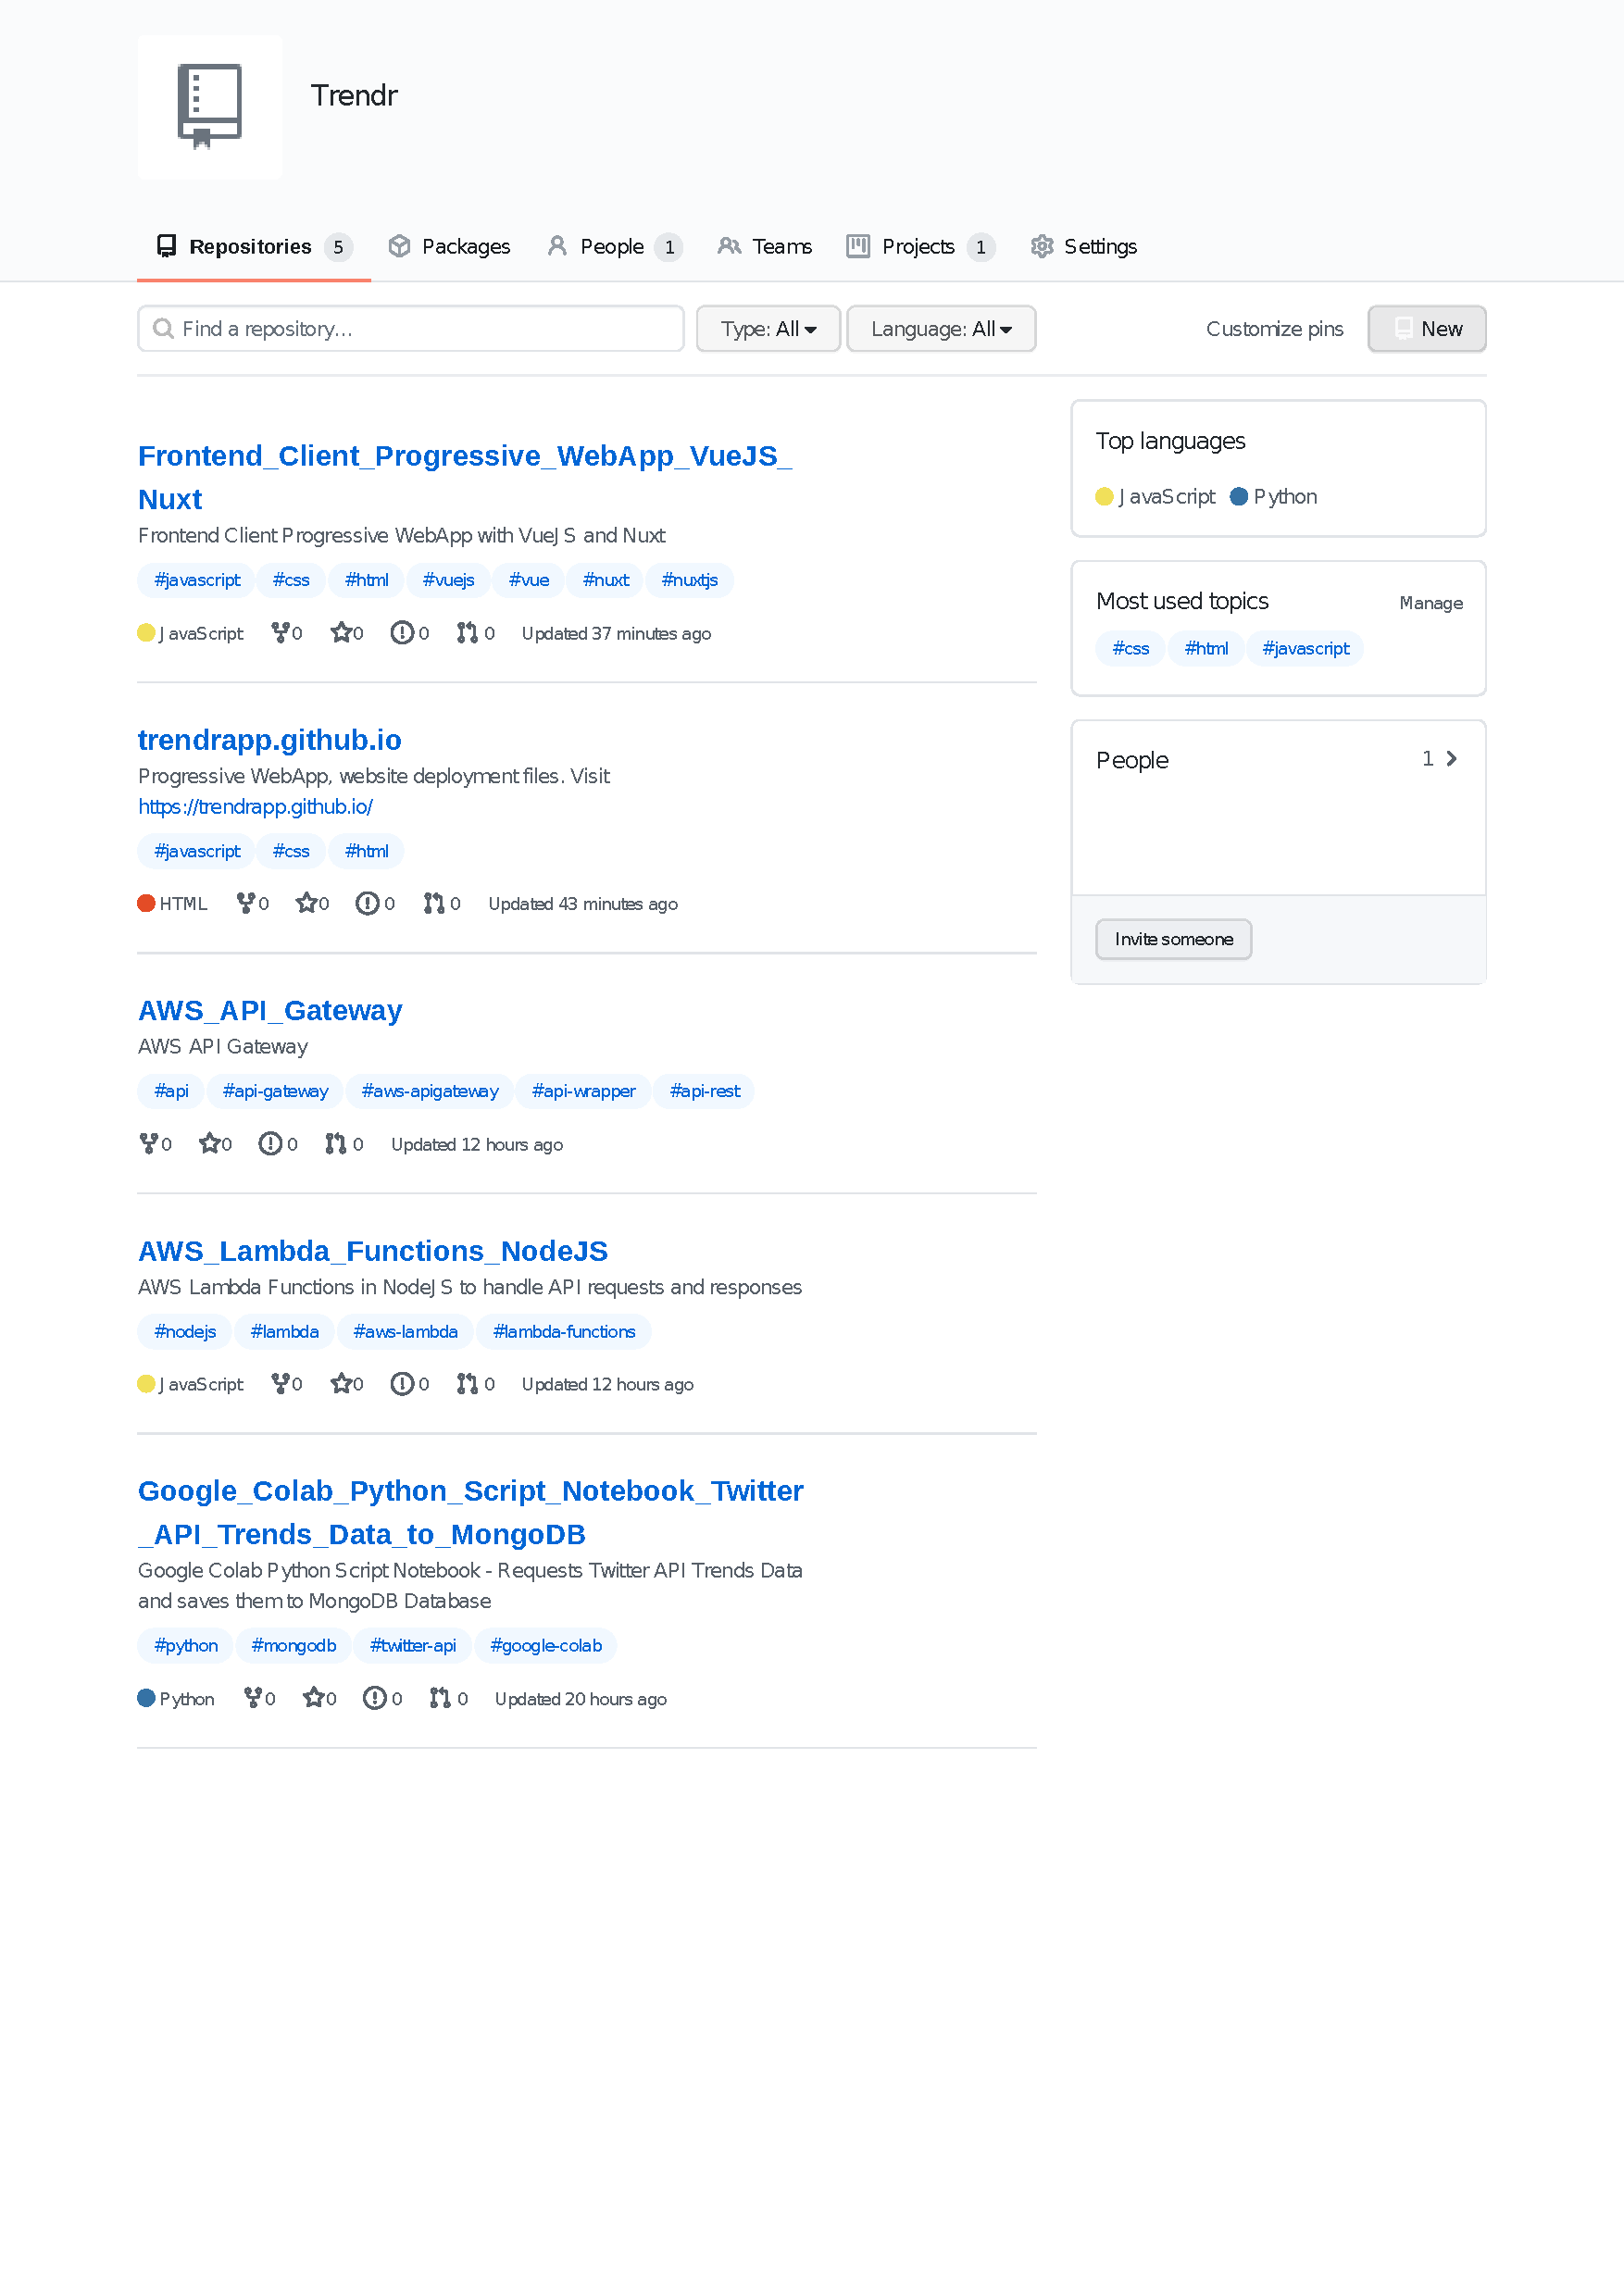
\includegraphics[width=0.75\paperwidth,height=0.87\paperheight,keepaspectratio]{Github_Repos.pdf}
    \end{figure}
\end{frame}

%------------------------------------------------

\subsection{Descrizione del progetto}

\subsubsection{Lato BackEnd}

\begin{frame}{Descrizione del progetto (BackEnd)}
    \begin{block}{Il progetto consiste di un lato BackEnd in cui si effettuano:}
        \begin{itemize}
            \item Acquisizione dei Trending Topics di Twitter dal suo API mediante uno script (Python).
            \item Salvataggio dei dati in un Database NoSQL (MongoDB).
            \item Esposizione di un API Gateway per l'accesso ai dati salvati tramite client.
            \item Gestione mediante Lambda Functions (NodeJS) delle richieste provenienti dall'API Gateway.
            \item Invio delle response a tali richieste con dati strutturati.
        \end{itemize}
    \end{block}
\end{frame}

%------------------------------------------------

\subsubsection{Lato FrontEnd}

\begin{frame}{Descrizione del progetto (FrontEnd)}
    \begin{block}{Inoltre c'è un lato FrontEnd in cui si effettuano:}
        \begin{itemize}
            \item Interrogazione dell'API Gateway tramite una Progressive WebApp.
            \item Visualizzazione dei Trending Topics ricevuti come risposta delle interrogazioni.
        \end{itemize}
    \end{block}
    
    \begin{block}{Il lato client è sviluppato come una Progressive WebApp}
        Il sito è:
        \begin{itemize}
            \item visualizzabile da qualsiasi client browser desktop
            \item visualizzabile da browser mobile in modo responsive
            \item installabile come Progressive WebApp su dispositivi Android e iOS.
        \end{itemize}
    \end{block}
\end{frame}

%------------------------------------------------

\subsection{Architettura del progetto}

\subsubsection{Layout}

\begin{frame}{Layout del progetto}
    \vspace*{-56pt}
    \begin{figure}[H]
        \centering
        \noindent\makebox[\textheight]{
            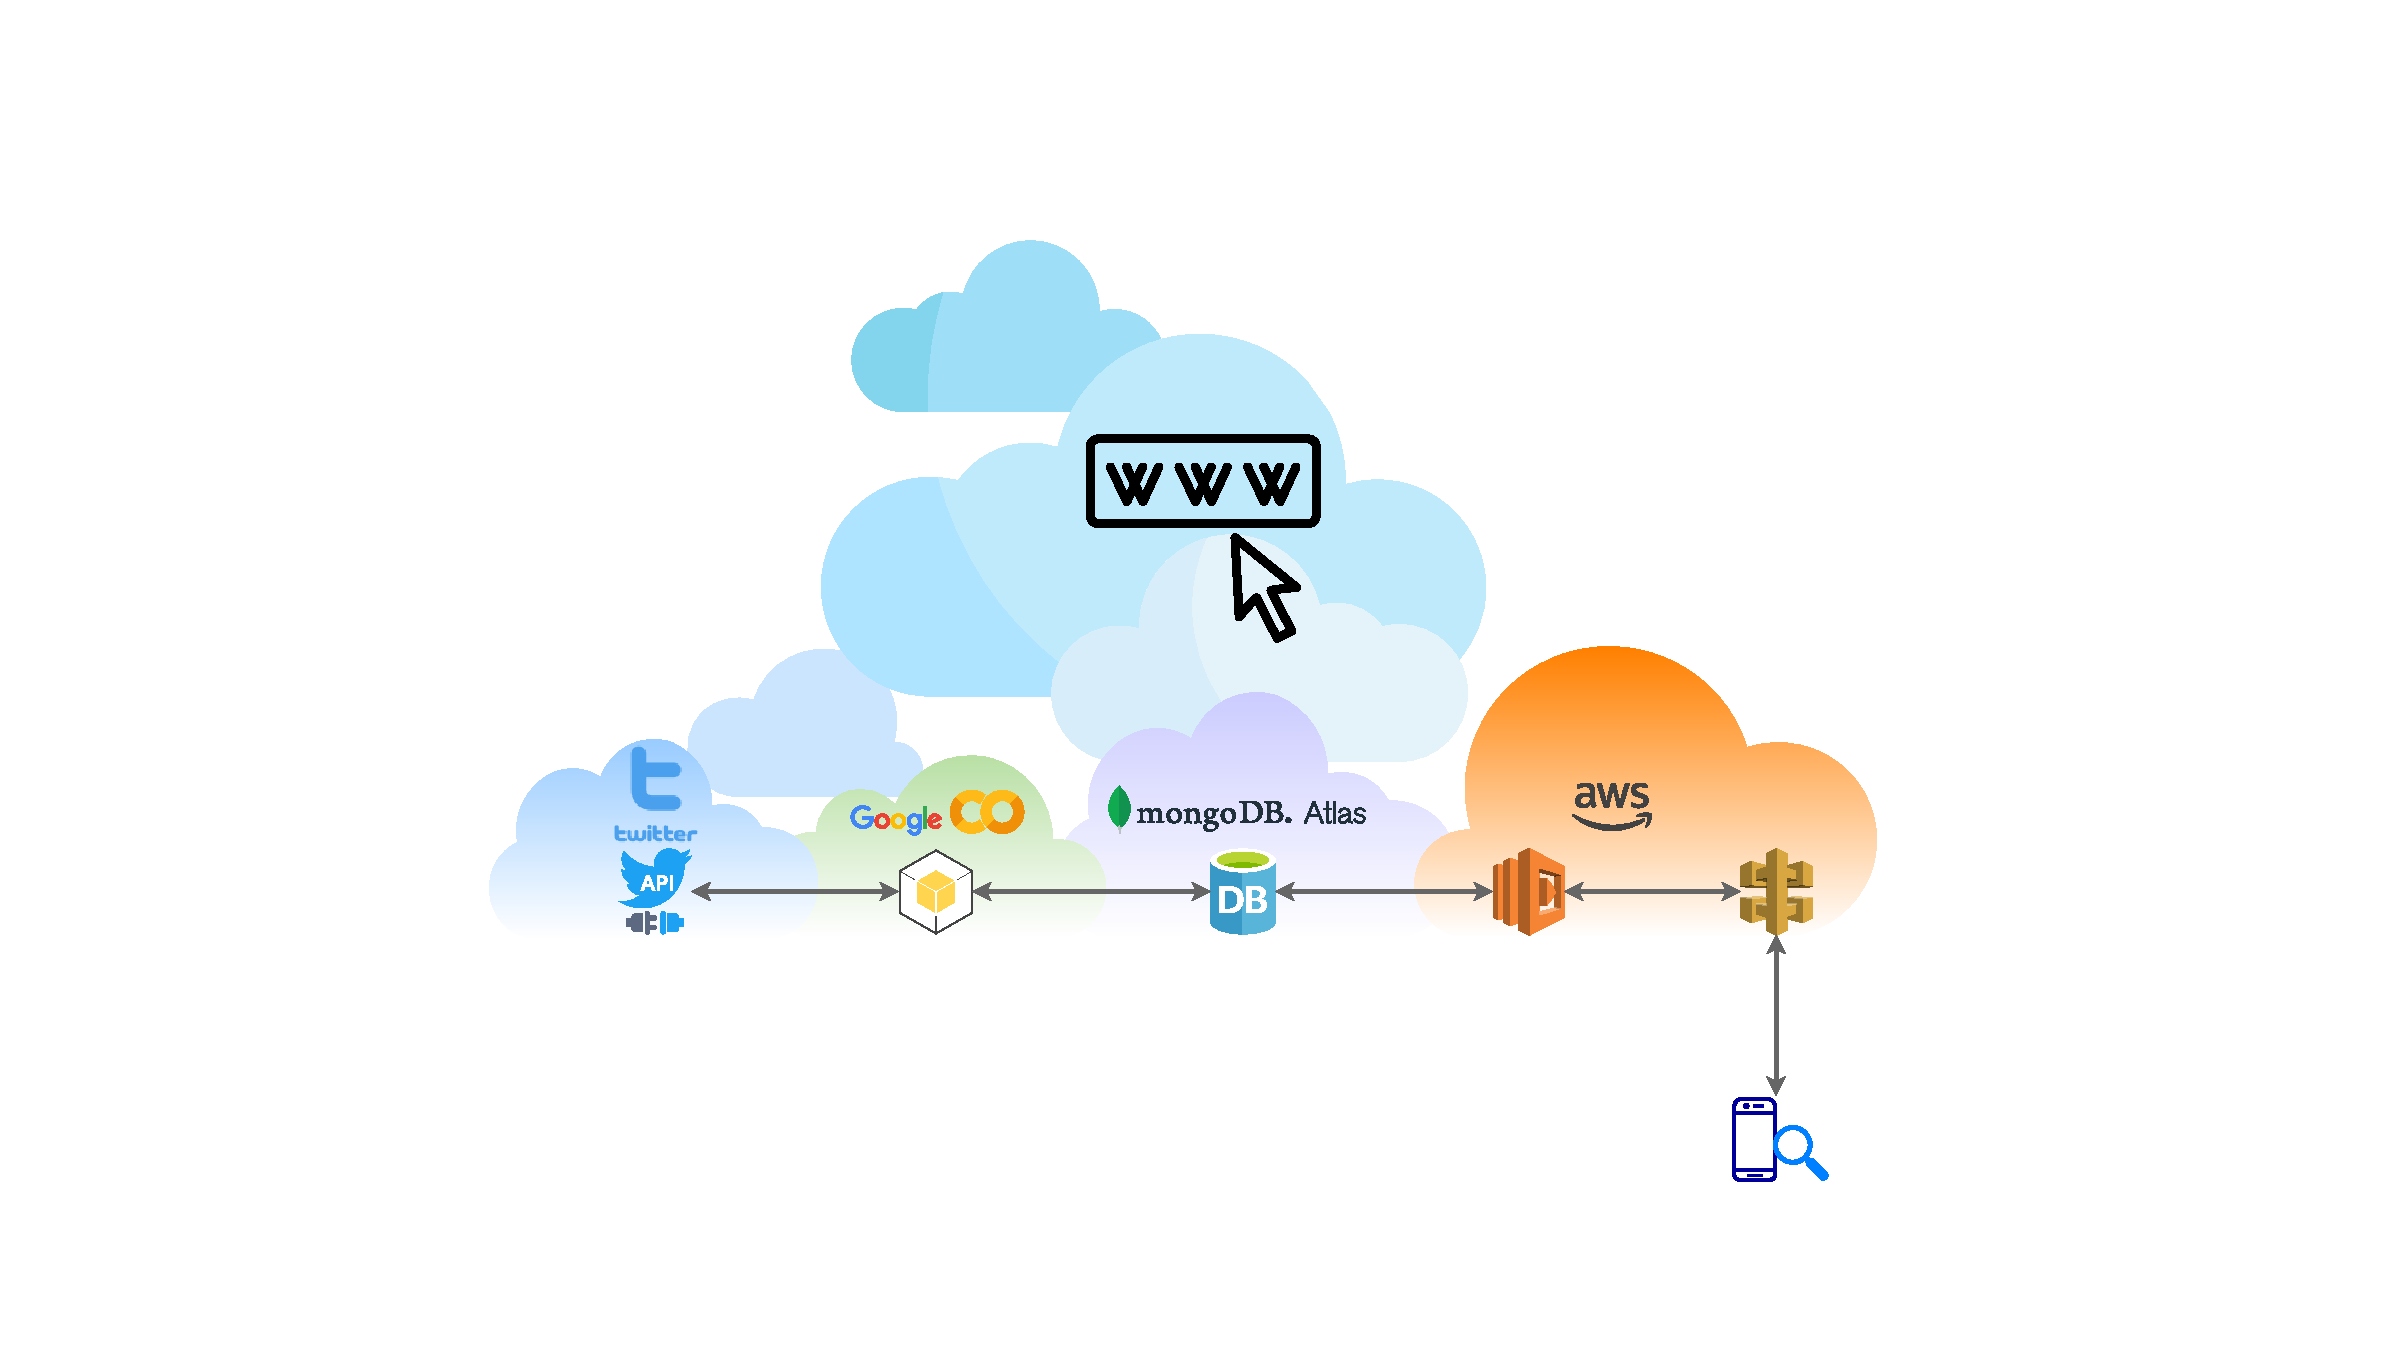
\includegraphics[width=1\paperwidth,height=1\paperheight,keepaspectratio]{Architectura_progetto_tutto_attivo.pdf}
        }
    \end{figure}
\end{frame}

%------------------------------------------------

\subsubsection{Tecnologie usate}

\begin{frame}{Tecnologie usate}
    \vspace*{-12pt}
    \begin{columns}[t] % The "c" option specifies centered vertical alignment while the "t" option is used for top vertical alignment
        \column{.475\textwidth}
        \begin{block}{Lato BackEnd}
            \begin{itemize}
                \item Python, Google Colab Notebooks
                \item MongoDB
                \item AWS API Gateway
                \item AWS Lambda Functions
                \item Javascript, NodeJS, JSON
                \item Postman
                \item PyCharm IDE
            \end{itemize}
        \end{block}
        
        \column{.475\textwidth}
        \begin{block}{Lato FrontEnd}
            \begin{itemize}
                \item HTML, CSS, Javascript, JSON
                \item NodeJS, VueJS, Nuxt
                \item Android OS, iOS
                \item WebStorm IDE \& Chrome DevTools
            \end{itemize}
        \end{block}
        \begin{block}{Deployment}
            \begin{itemize}
                \item GitHub Pages
            \end{itemize}
        \end{block}
    \end{columns}
    \begin{columns}[t] % The "c" option specifies centered vertical alignment while the "t" option is used for top vertical alignment
        \column{0.98\textwidth}
        \begin{block}{Presentazione}
            \begin{itemize}
                \item Latex, Beamer, Overleaf, Draw.io, Inkscape
            \end{itemize}
        \end{block}
    \end{columns}
\end{frame}

%------------------------------------------------

\section{BackEnd}

\begin{frame}{\secname}
    \tableofcontents[sections={\thesection}, subsubsectionstyle=show, sectionstyle=hide]
\end{frame}

%------------------------------------------------

\subsection{Dati ottenuti da Twitter API}

\begin{frame}{Twitter API}
    \vspace*{-56pt}
    \begin{figure}[H]
        \centering
        \noindent\makebox[\textheight]{
            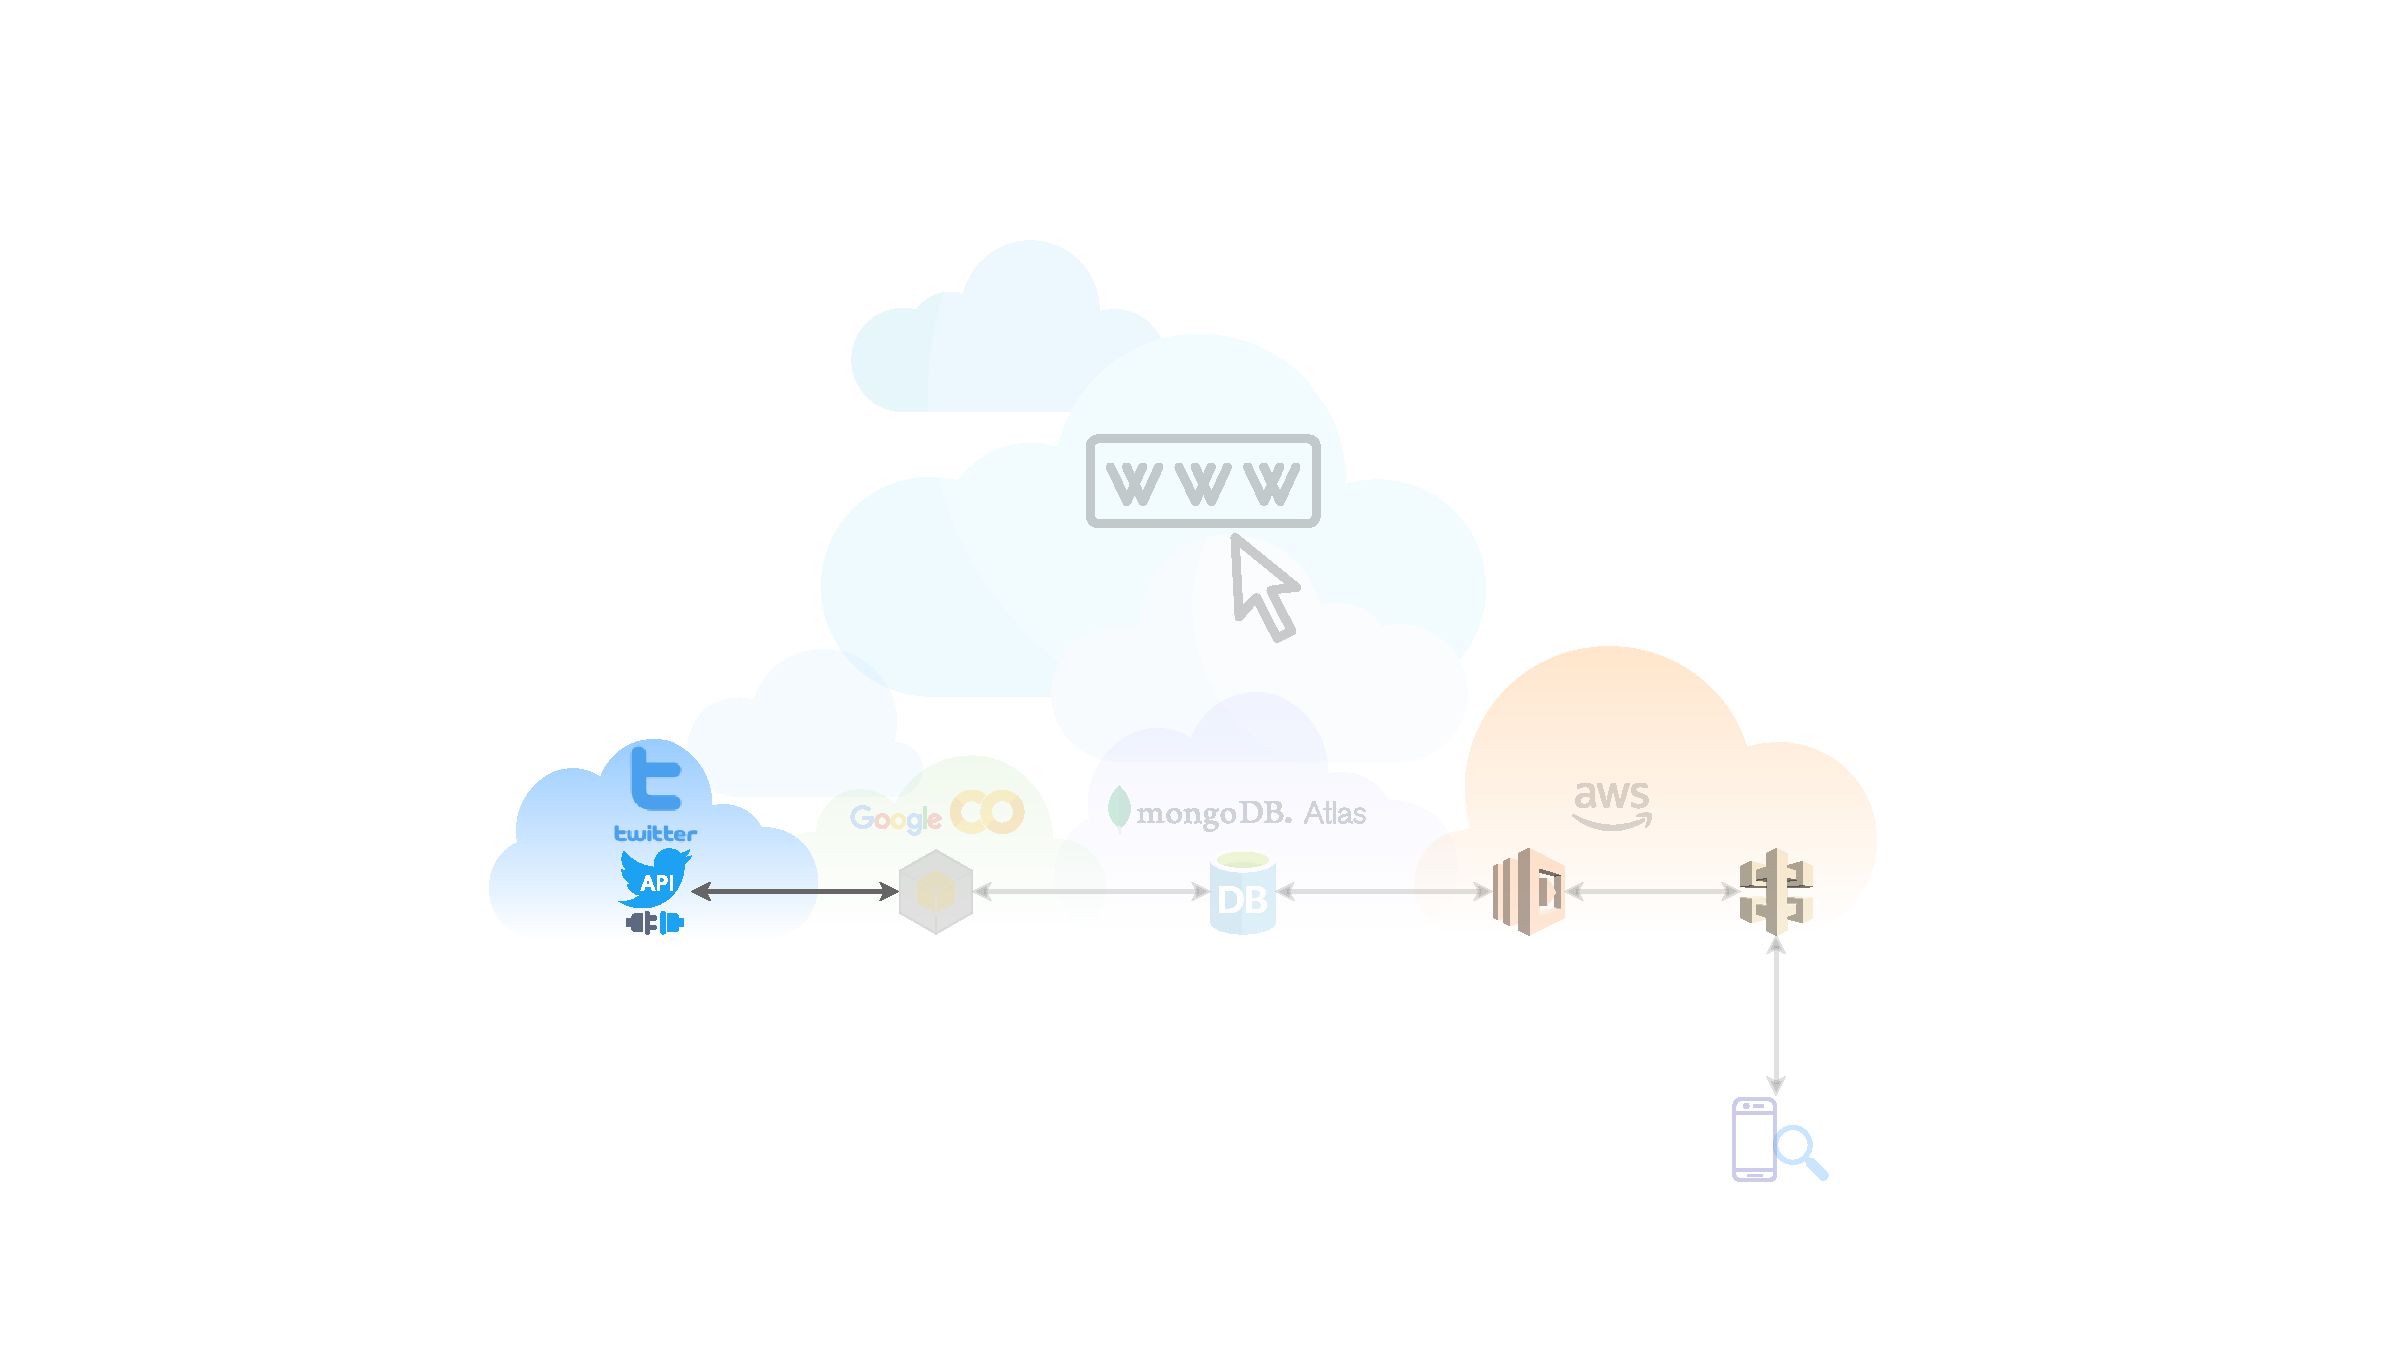
\includegraphics[width=1\paperwidth,height=1\paperheight,keepaspectratio]{Architectura_progetto_Twitter_API.pdf}
        }
    \end{figure}
\end{frame}

\subsubsection{Twitter Trending Topics}

\begin{frame}{Twitter Trending Topics}
    \fontsize{10pt}{10}\selectfont
    \begin{columns}[t]
        \column{.31\textwidth}
        I trending topics sono gli argomenti di cui più si parla in un determinato momento su Twitter, in una determinata località.\\~\\~\\~\\~\\
        
        Twitter usa degli algoritmi per raggruppare le tendenze e gli hashtag correlati allo stesso argomento.
        \column{.64\textwidth}
        \vspace*{-48pt}
        \begin{figure}[H]
            \centering
            \noindent\makebox[\textheight]{
                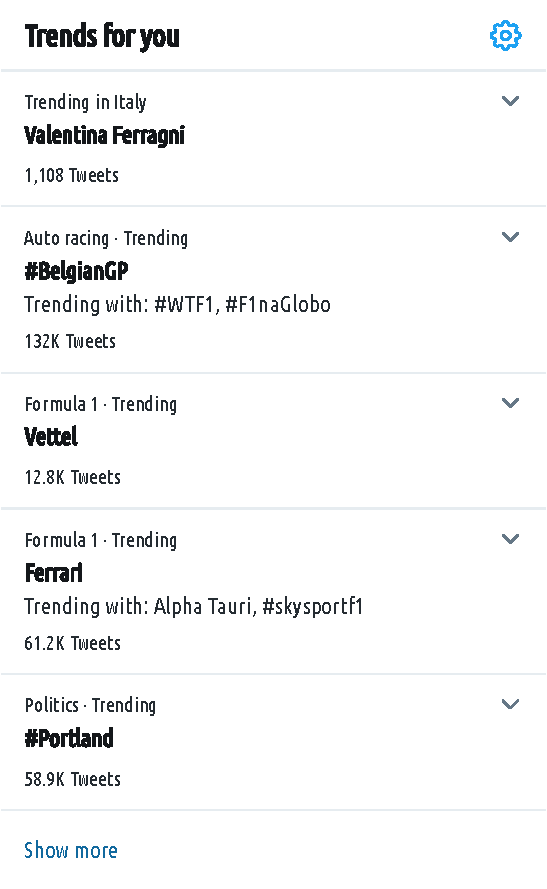
\includegraphics[width=0.64\paperwidth,height=0.75\paperheight,keepaspectratio]{Twitter_Trending_Topics.pdf}
            }
        \end{figure}
    \end{columns}
\end{frame}

%------------------------------------------------

\begin{frame}{Twitter TT, cosa manca}
    \fontsize{10pt}{10}\selectfont
    Twitter offre tramite la sua API la possibilità di accedere ai suoi trending topics del momento.\\~\\~\\~\\~\\
    
    Le API di Twitter però non offrono la possibilità di vedere i trending topics del passato.\\~\\~\\~\\~\\
    
    Inoltre è possibile vedere i TT del momento di località diverse dalla propria solo se si è già registrati e loggati su Twitter.
\end{frame}

%------------------------------------------------

\subsubsection{GET Locations aventi Trending Topics e i relativi Trends}

\begin{frame}{GET Available Locations}
    \fontsize{10pt}{10}\selectfont
    \begin{columns}[t]
        \column{.31\textwidth}
        Via le Twitter APIs, si può ricavare un JSON contenente un elenco delle locations nelle quali al momento ci sono trending topics.\\~\\~\\~\\~\\
        
        Ogni location (che sia paese o città) ha un suo WOEID (Where on Earth ID).
        
        \column{.64\textwidth}
        \vspace*{-48pt}
        \begin{figure}[H]
            \centering
            \noindent\makebox[\textheight]{
                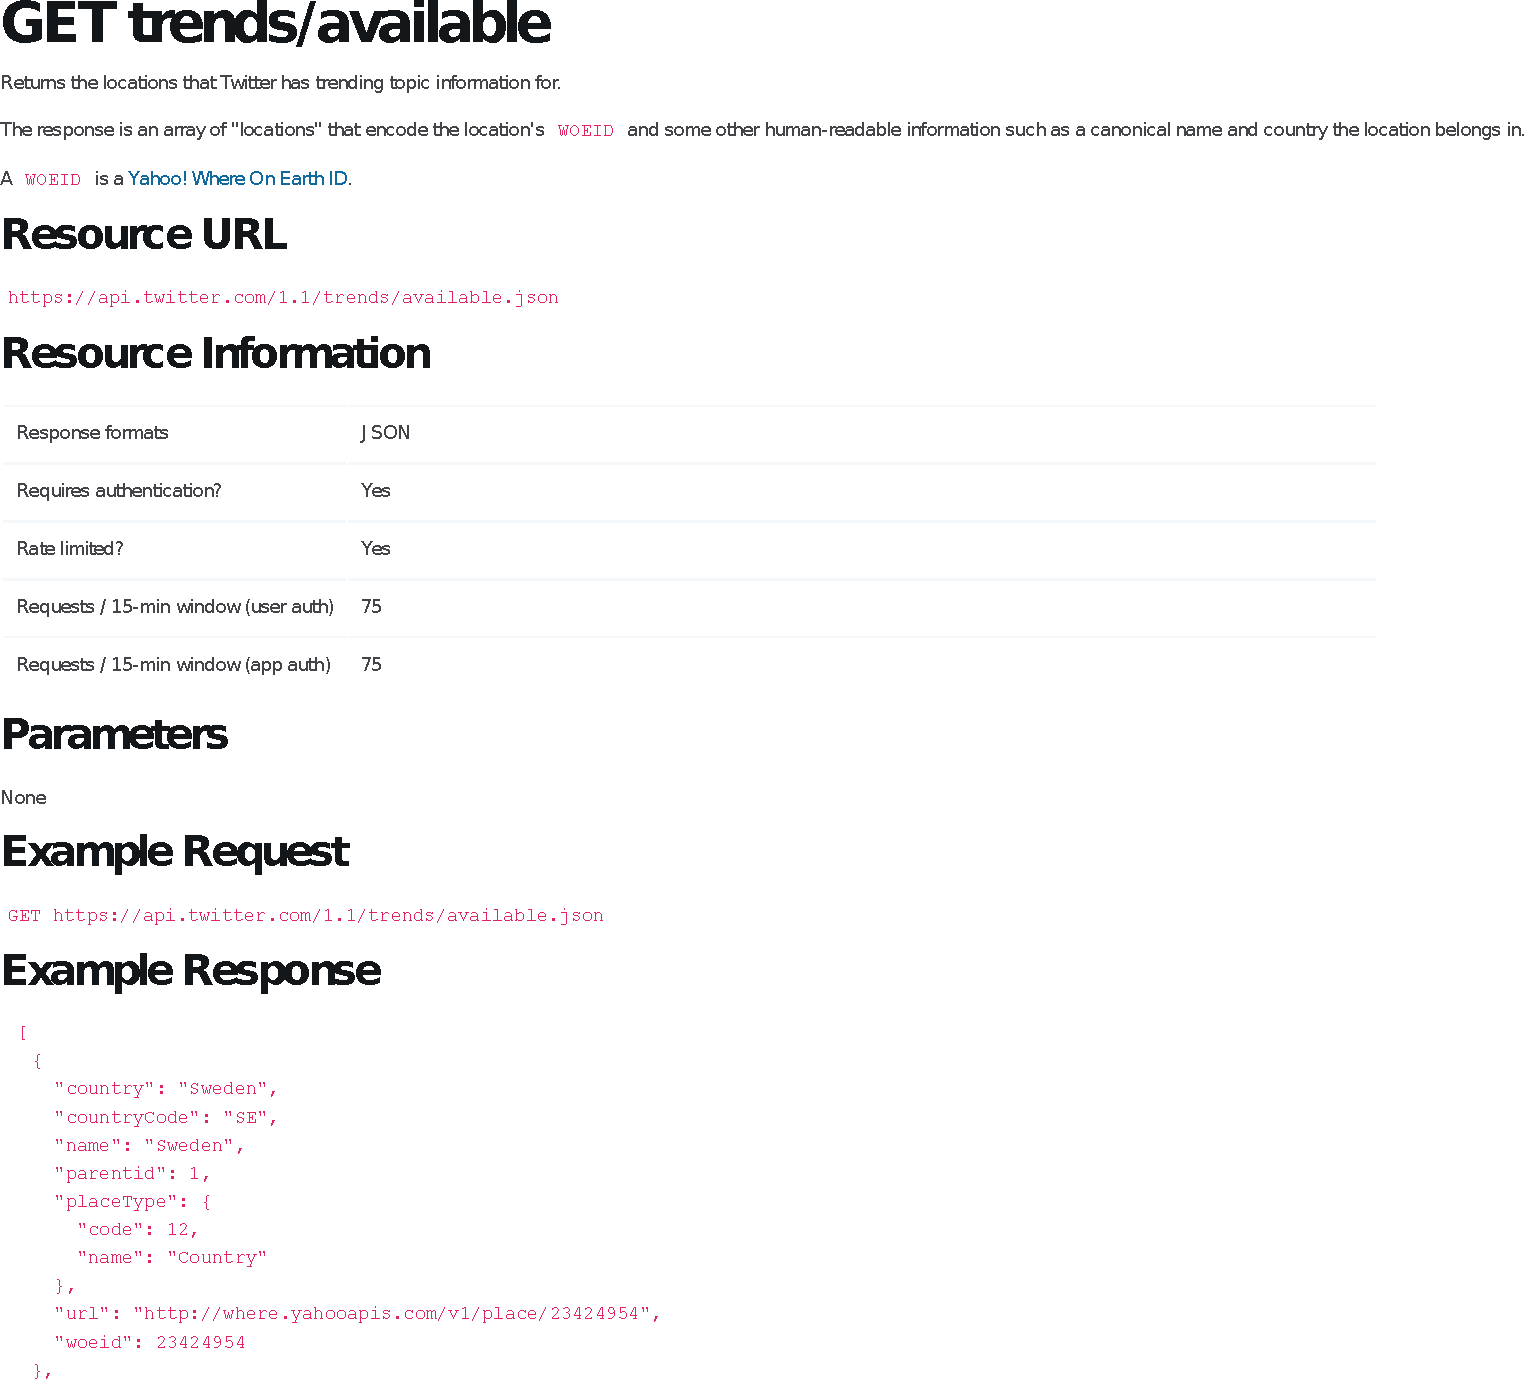
\includegraphics[width=0.64\paperwidth,height=0.75\paperheight,keepaspectratio]{Twitter_API_GET_Locations_with_Trends.pdf}
            }
        \end{figure}
    \end{columns}
\end{frame}

%------------------------------------------------

\begin{frame}{GET Trends}
    \fontsize{10pt}{10}\selectfont
    \begin{columns}[t]
        \column{.31\textwidth}
        Una volta ottenuto l'elenco delle locations nelle quali al momento ci sono trending topics, interroghiamo l'API di Twitter per ricavare i trends in ciascuna delle locations.\\~\\~\\~\\~\\
        
        L'unico parametro richiesto è l'WOEID della location.
        
        \column{.64\textwidth}
        \vspace*{-48pt}
        \begin{figure}[H]
            \centering
            \noindent\makebox[\textheight]{
                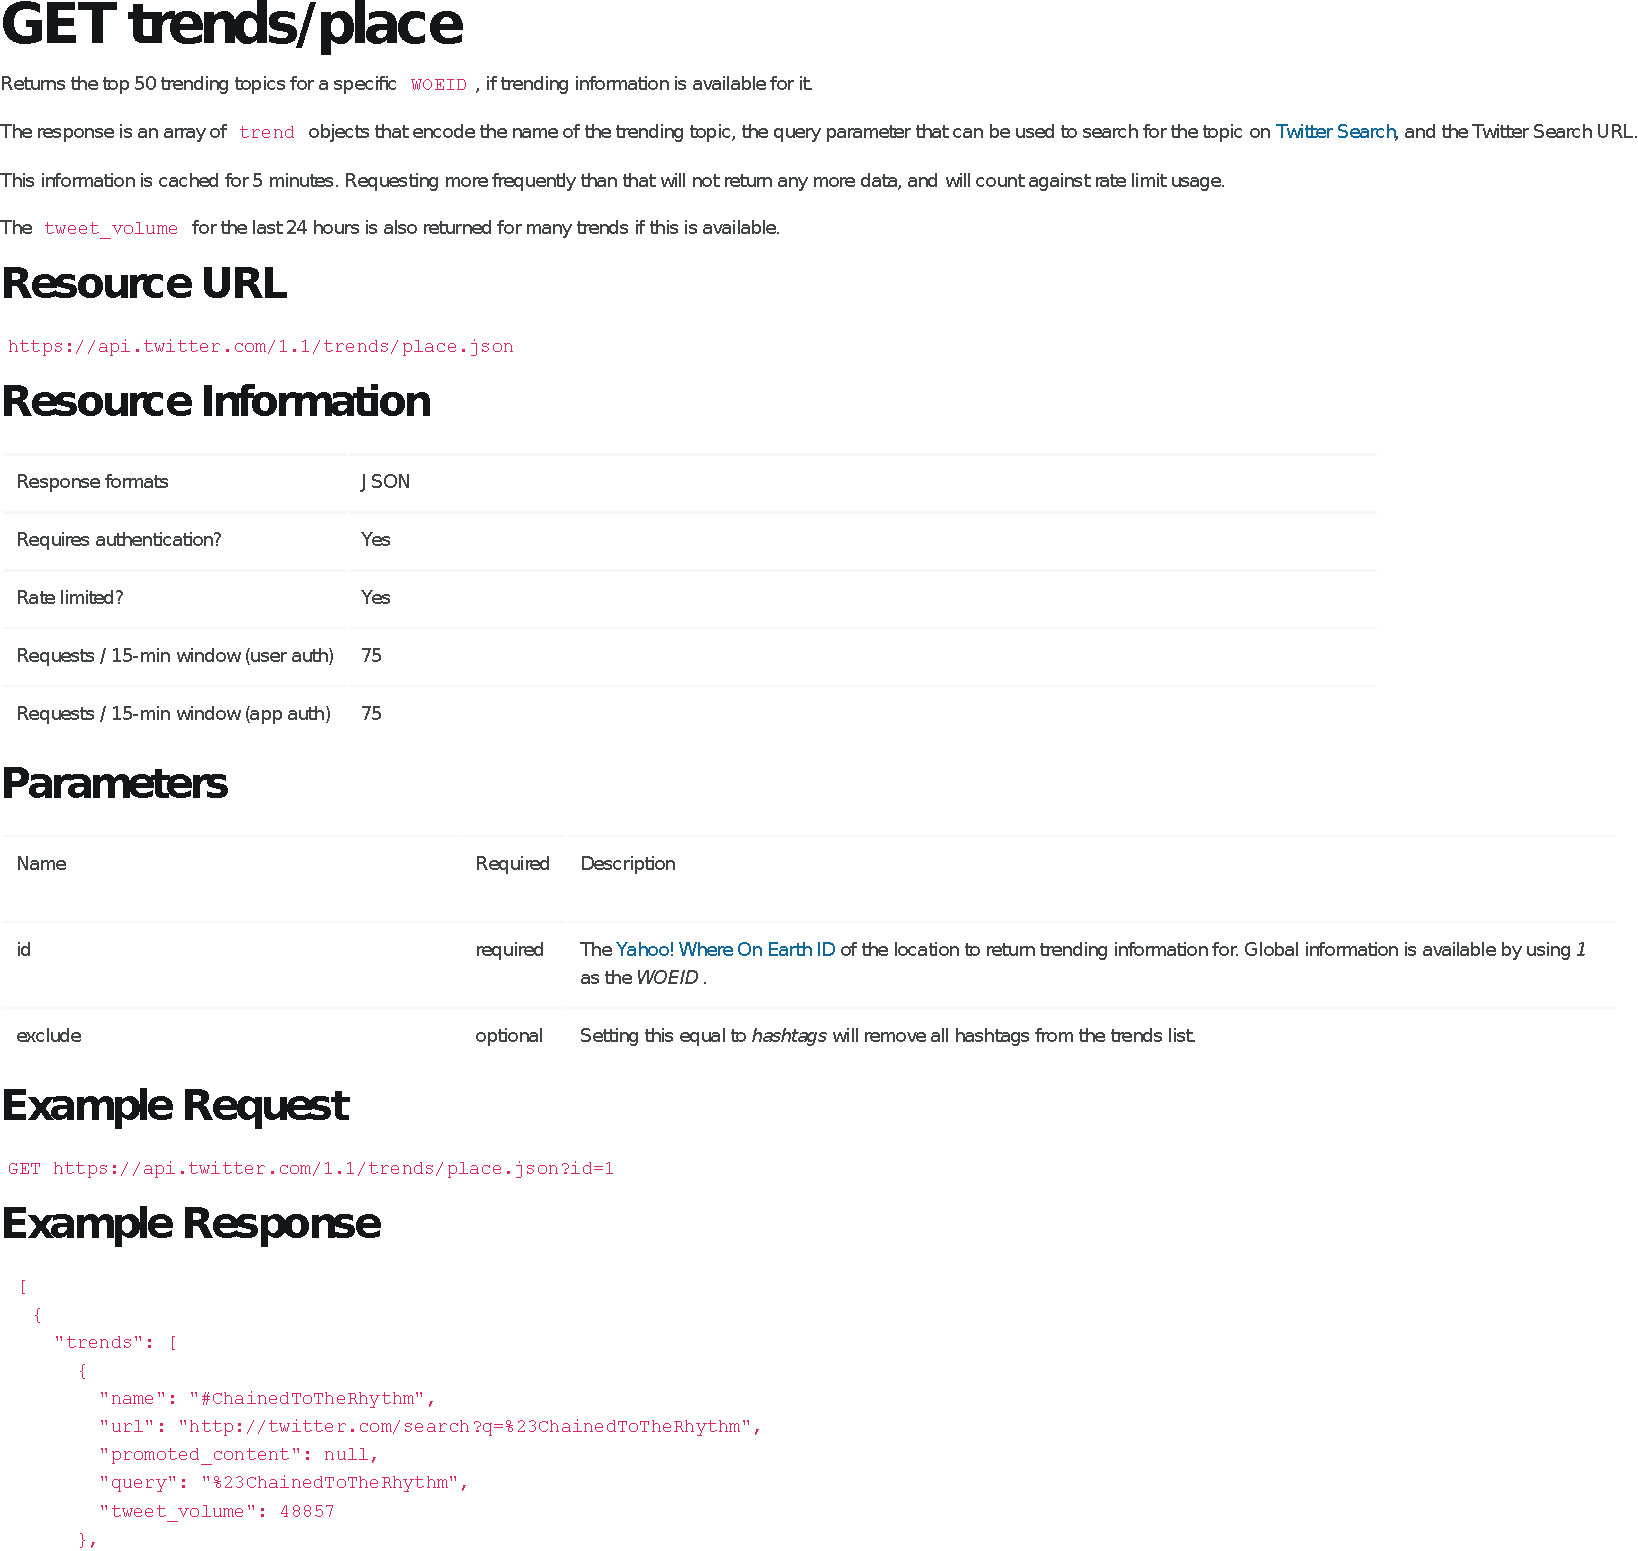
\includegraphics[width=0.64\paperwidth,height=0.75\paperheight,keepaspectratio]{Twitter_API_GET_Trends.pdf}
            }
        \end{figure}
    \end{columns}
\end{frame}

%------------------------------------------------

\subsubsection{Limiti del request rate di Twitter API }

\begin{frame}{Twitter API Rate limits}
    \fontsize{10pt}{10}\selectfont
    \begin{columns}[t]
        \column{.31\textwidth}
        L'accesso a questi dati è limitato ad un numero massimo di requests per utente o app ogni 15 minuti.\\~\\~\\~\\~\\
        
        Nello sviluppo dello script Python in Google Colab notebook per l'interrogazione di Twitter APIs e il salvataggio dei dati in MongoDB, si rispetta tale limite mantenendo una moderata rate di invio di requests per permettere il reset delle richieste allotted.
        
        \column{.64\textwidth}
        \vspace*{-48pt}
        \begin{figure}[H]
            \centering
            \noindent\makebox[\textheight]{
                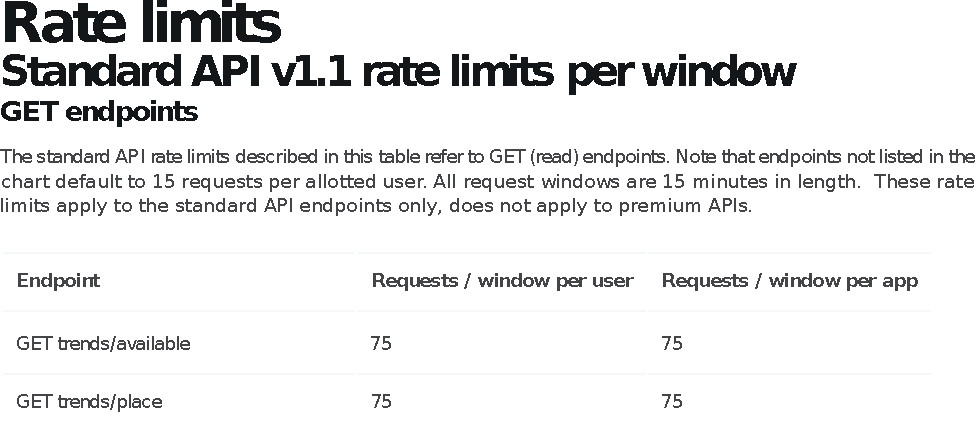
\includegraphics[width=0.5\paperwidth,height=0.64\paperheight,keepaspectratio]{Twitter_API_Rate_limits.pdf}
            }
        \end{figure}
    \end{columns}
\end{frame}

%------------------------------------------------

\subsection{Dati salvati su MongoDB Database}

\begin{frame}{MongoDB Atlas}
    \vspace*{-56pt}
    \begin{figure}[H]
        \centering
        \noindent\makebox[\textheight]{
            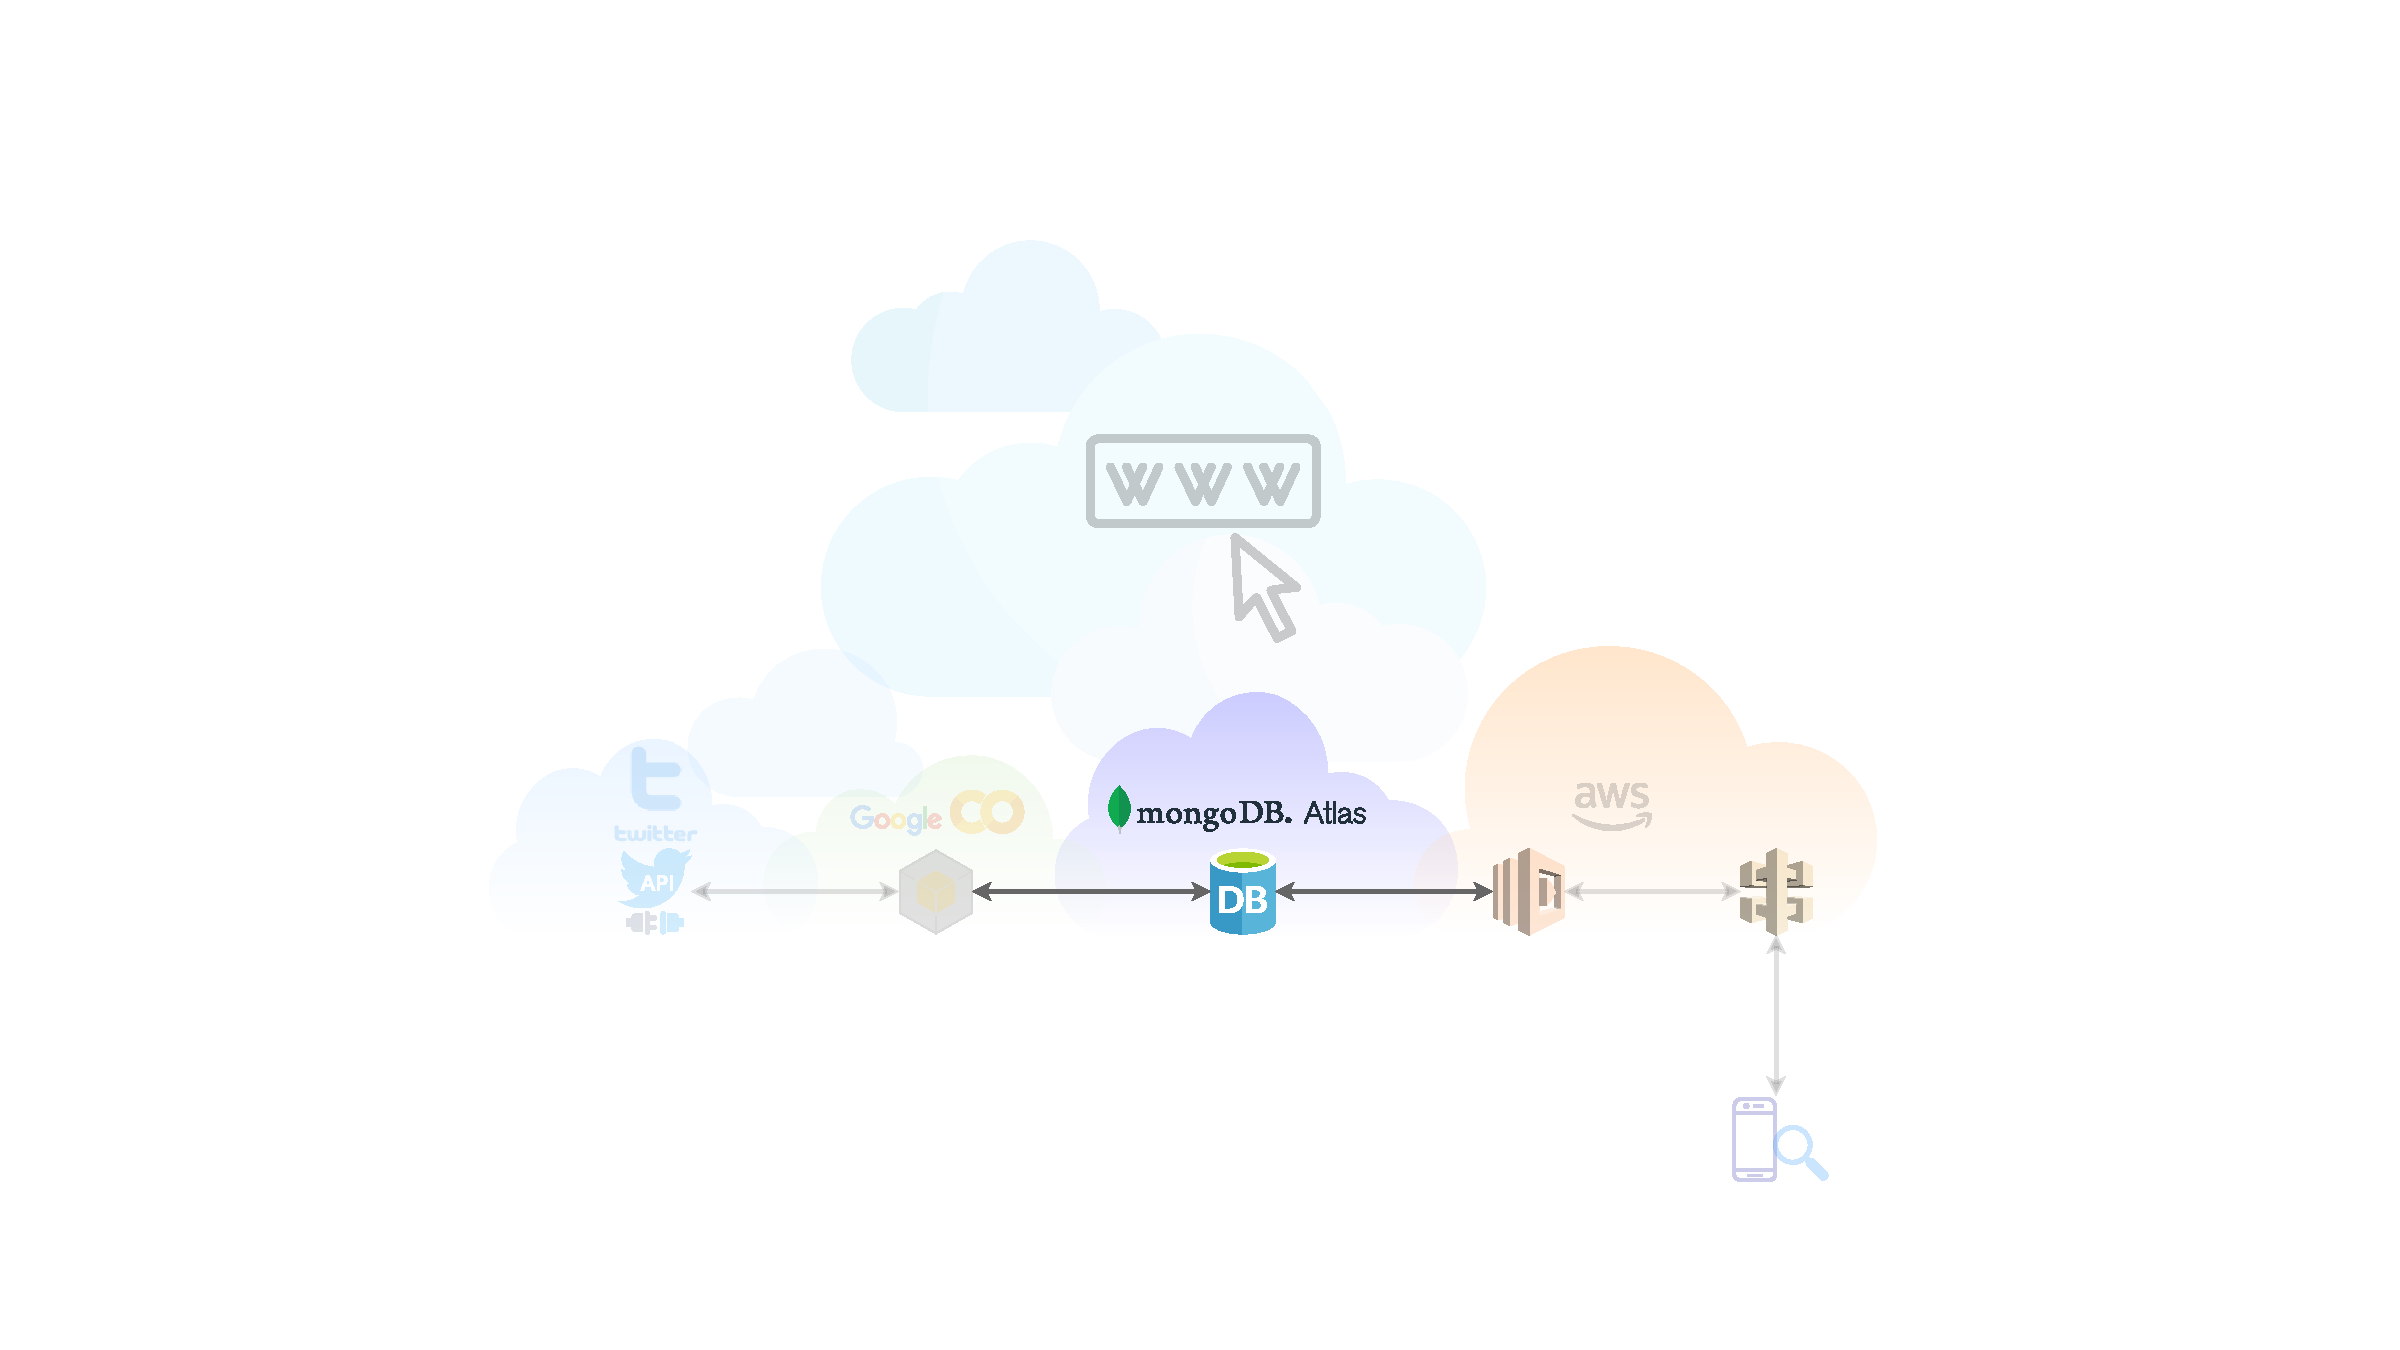
\includegraphics[width=1\paperwidth,height=1\paperheight,keepaspectratio]{Architectura_progetto_MongoDB.pdf}
        }
    \end{figure}
\end{frame}

%------------------------------------------------

\begin{frame}
    \begin{figure}[H]
        \centering
        \noindent\makebox[\textheight]{
            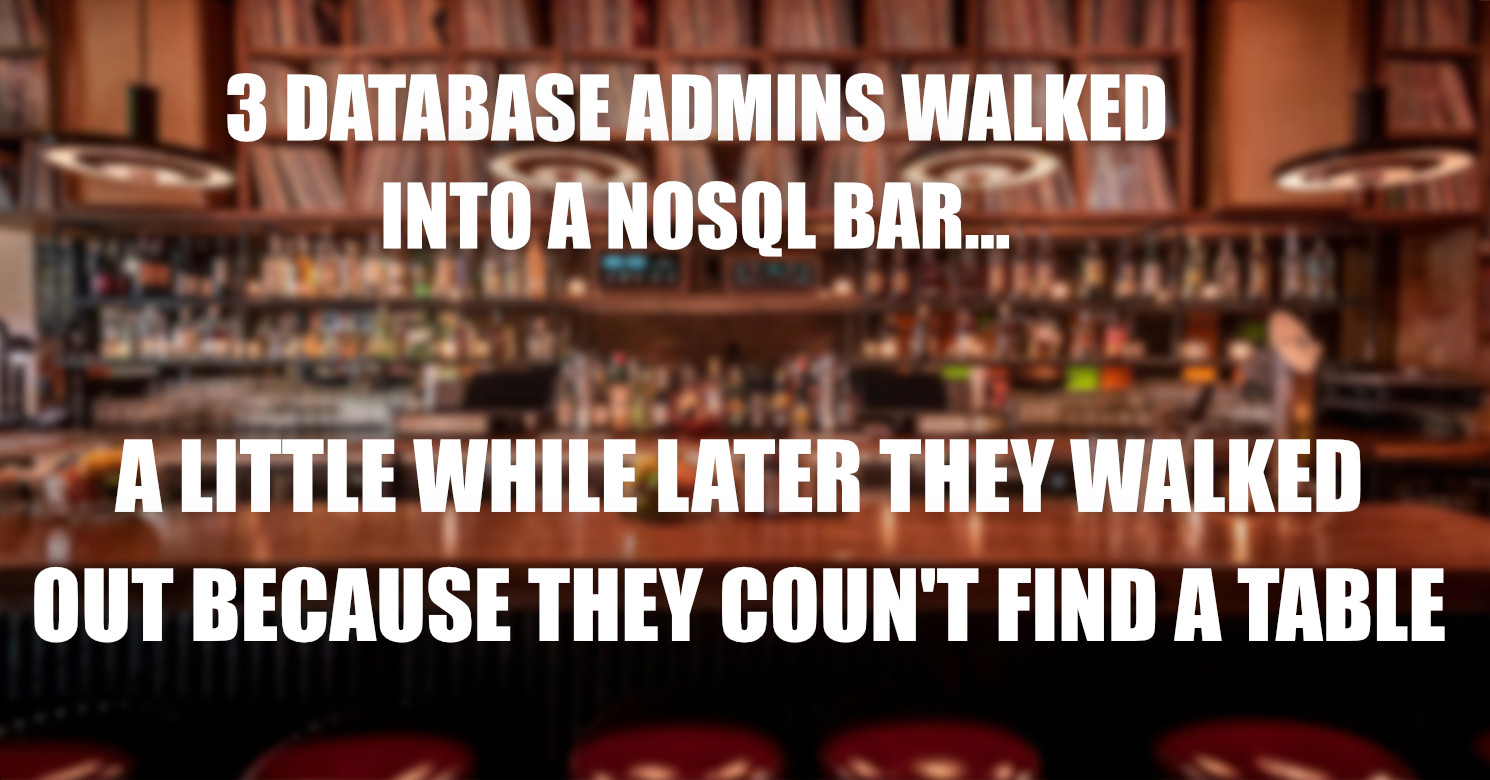
\includegraphics[width=0.8\paperwidth,height=0.8\paperheight,keepaspectratio]{Meme_NoSQL.jpg}
        }
    \end{figure}
\end{frame}

%------------------------------------------------

\subsubsection{Il database e le collezioni di dati}

\begin{frame}{Il cluster}
    \begin{columns}[t]
        \column{.31\textwidth}
        Per cluster in MongoDB si intende sharded cluster. Il motivo è lo scaling delle letture e scritture lungo diversi nodi. Ogni nodo non gestisce tutti i dati.
        
        \column{.64\textwidth}
        \vspace*{-32pt}
        \begin{figure}[H]
            \centering
            \noindent\makebox[\textheight]{
                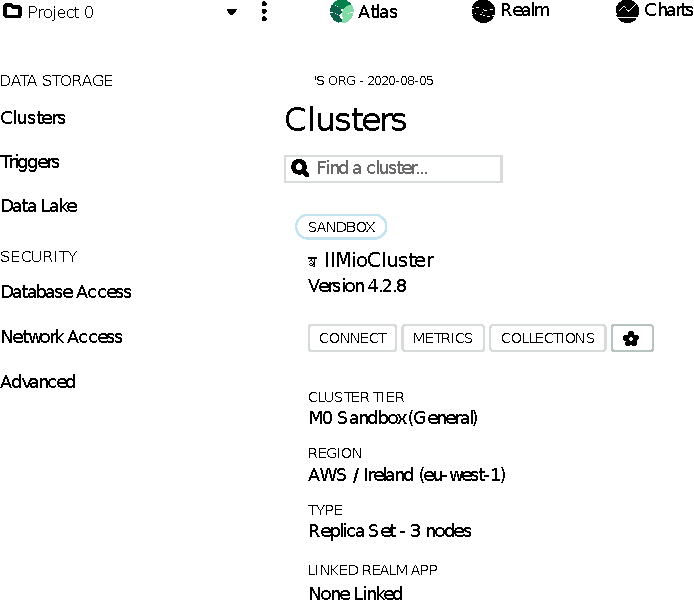
\includegraphics[width=0.5\paperwidth,height=0.5\paperheight,keepaspectratio]{MongoDB_Clusters.pdf}
            }
        \end{figure}
    \end{columns}
\end{frame}

%------------------------------------------------

\begin{frame}{Il database e le collezioni}
    \begin{columns}[t]
        \column{.30\textwidth}
        Per il salvataggio (e successiva lettura più aggevole) dei dati delle trending topics e delle locations si fa uso di un database con due collections, una per i trends e l'altra per le località.
        
        \column{.64\textwidth}
        \vspace*{-32pt}
        \begin{figure}[H]
            \centering
            \noindent\makebox[\textheight]{
                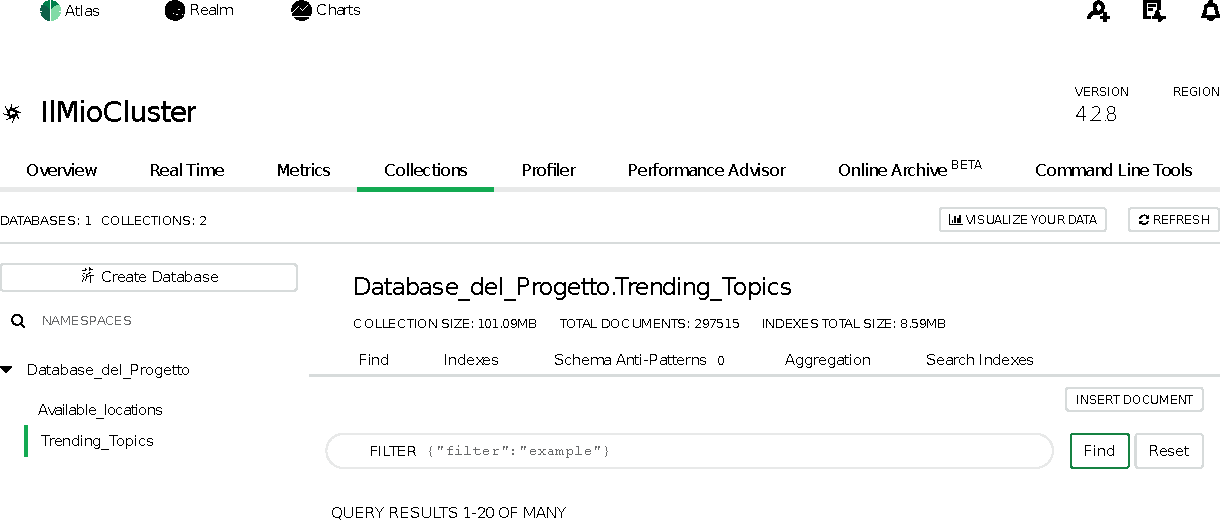
\includegraphics[width=0.64\paperwidth,height=0.64\paperheight,keepaspectratio]{MongoDB_Database_Collezioni.pdf}
            }
        \end{figure}
    \end{columns}
\end{frame}

%------------------------------------------------

\subsubsection{La struttura dei dati}

\begin{frame}{Formato dei dati in Available\_Locations}
    \begin{columns}[t]
        \column{.36\textwidth}
        \vspace*{32pt}
        
        La struttura dei dati inseriti nella collection delle località è composta da una data-ora, un oggetto "locations" con dentro "Worldwide", il suo WOEID e un array di paesi ciascuno con nome, WOEID e una lista delle proprie citta con relativo WOEID.
        
        \column{.59\textwidth}
        \vspace*{-45pt}
        \begin{figure}[H]
            \centering
            \noindent\makebox[\textheight]{
                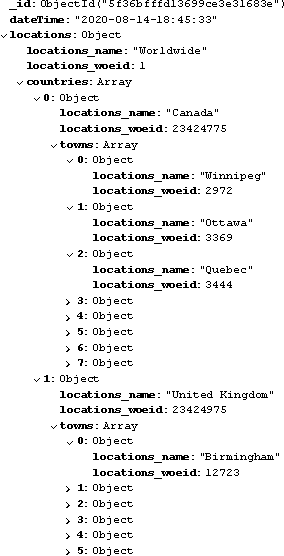
\includegraphics[width=0.59\paperwidth,height=0.9\paperheight,keepaspectratio]{MongoDB_Formato_Locations.pdf}
            }
        \end{figure}
    \end{columns}
\end{frame}

%------------------------------------------------

\begin{frame}{Formato dei dati in Trending\_Topics}
    \begin{columns}[t]
        \column{.31\textwidth}
        La struttura dei dati inseriti nella collection dei trends è composta da una data-ora di inserimento e creazione, nome della location, il tipo, WOEID, WOEID del genitore (genitore di città è paese, genitore di paese è worldwide). Inoltre ci sono i dati del topic come il nome o l'hashtag, l'url, se è un ad, la string query e il volume dei tweet che parlano di quell'argomento."
        
        \column{.64\textwidth}
        \vspace*{-16pt}
        \begin{figure}[H]
            \centering
            \noindent\makebox[\textheight]{
                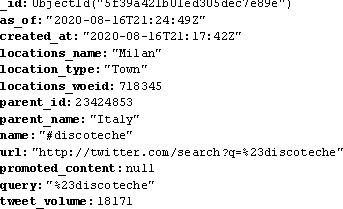
\includegraphics[width=0.5\paperwidth,height=0.5\paperheight,keepaspectratio]{MongoDB_Formato_Trends.pdf}
            }
        \end{figure}
    \end{columns}
\end{frame}

%------------------------------------------------

\subsection{Python script notebook su Google Colab}

\begin{frame}{Python notebook su Google Colab}
    \vspace*{-56pt}
    \begin{figure}[H]
        \centering
        \noindent\makebox[\textheight]{
            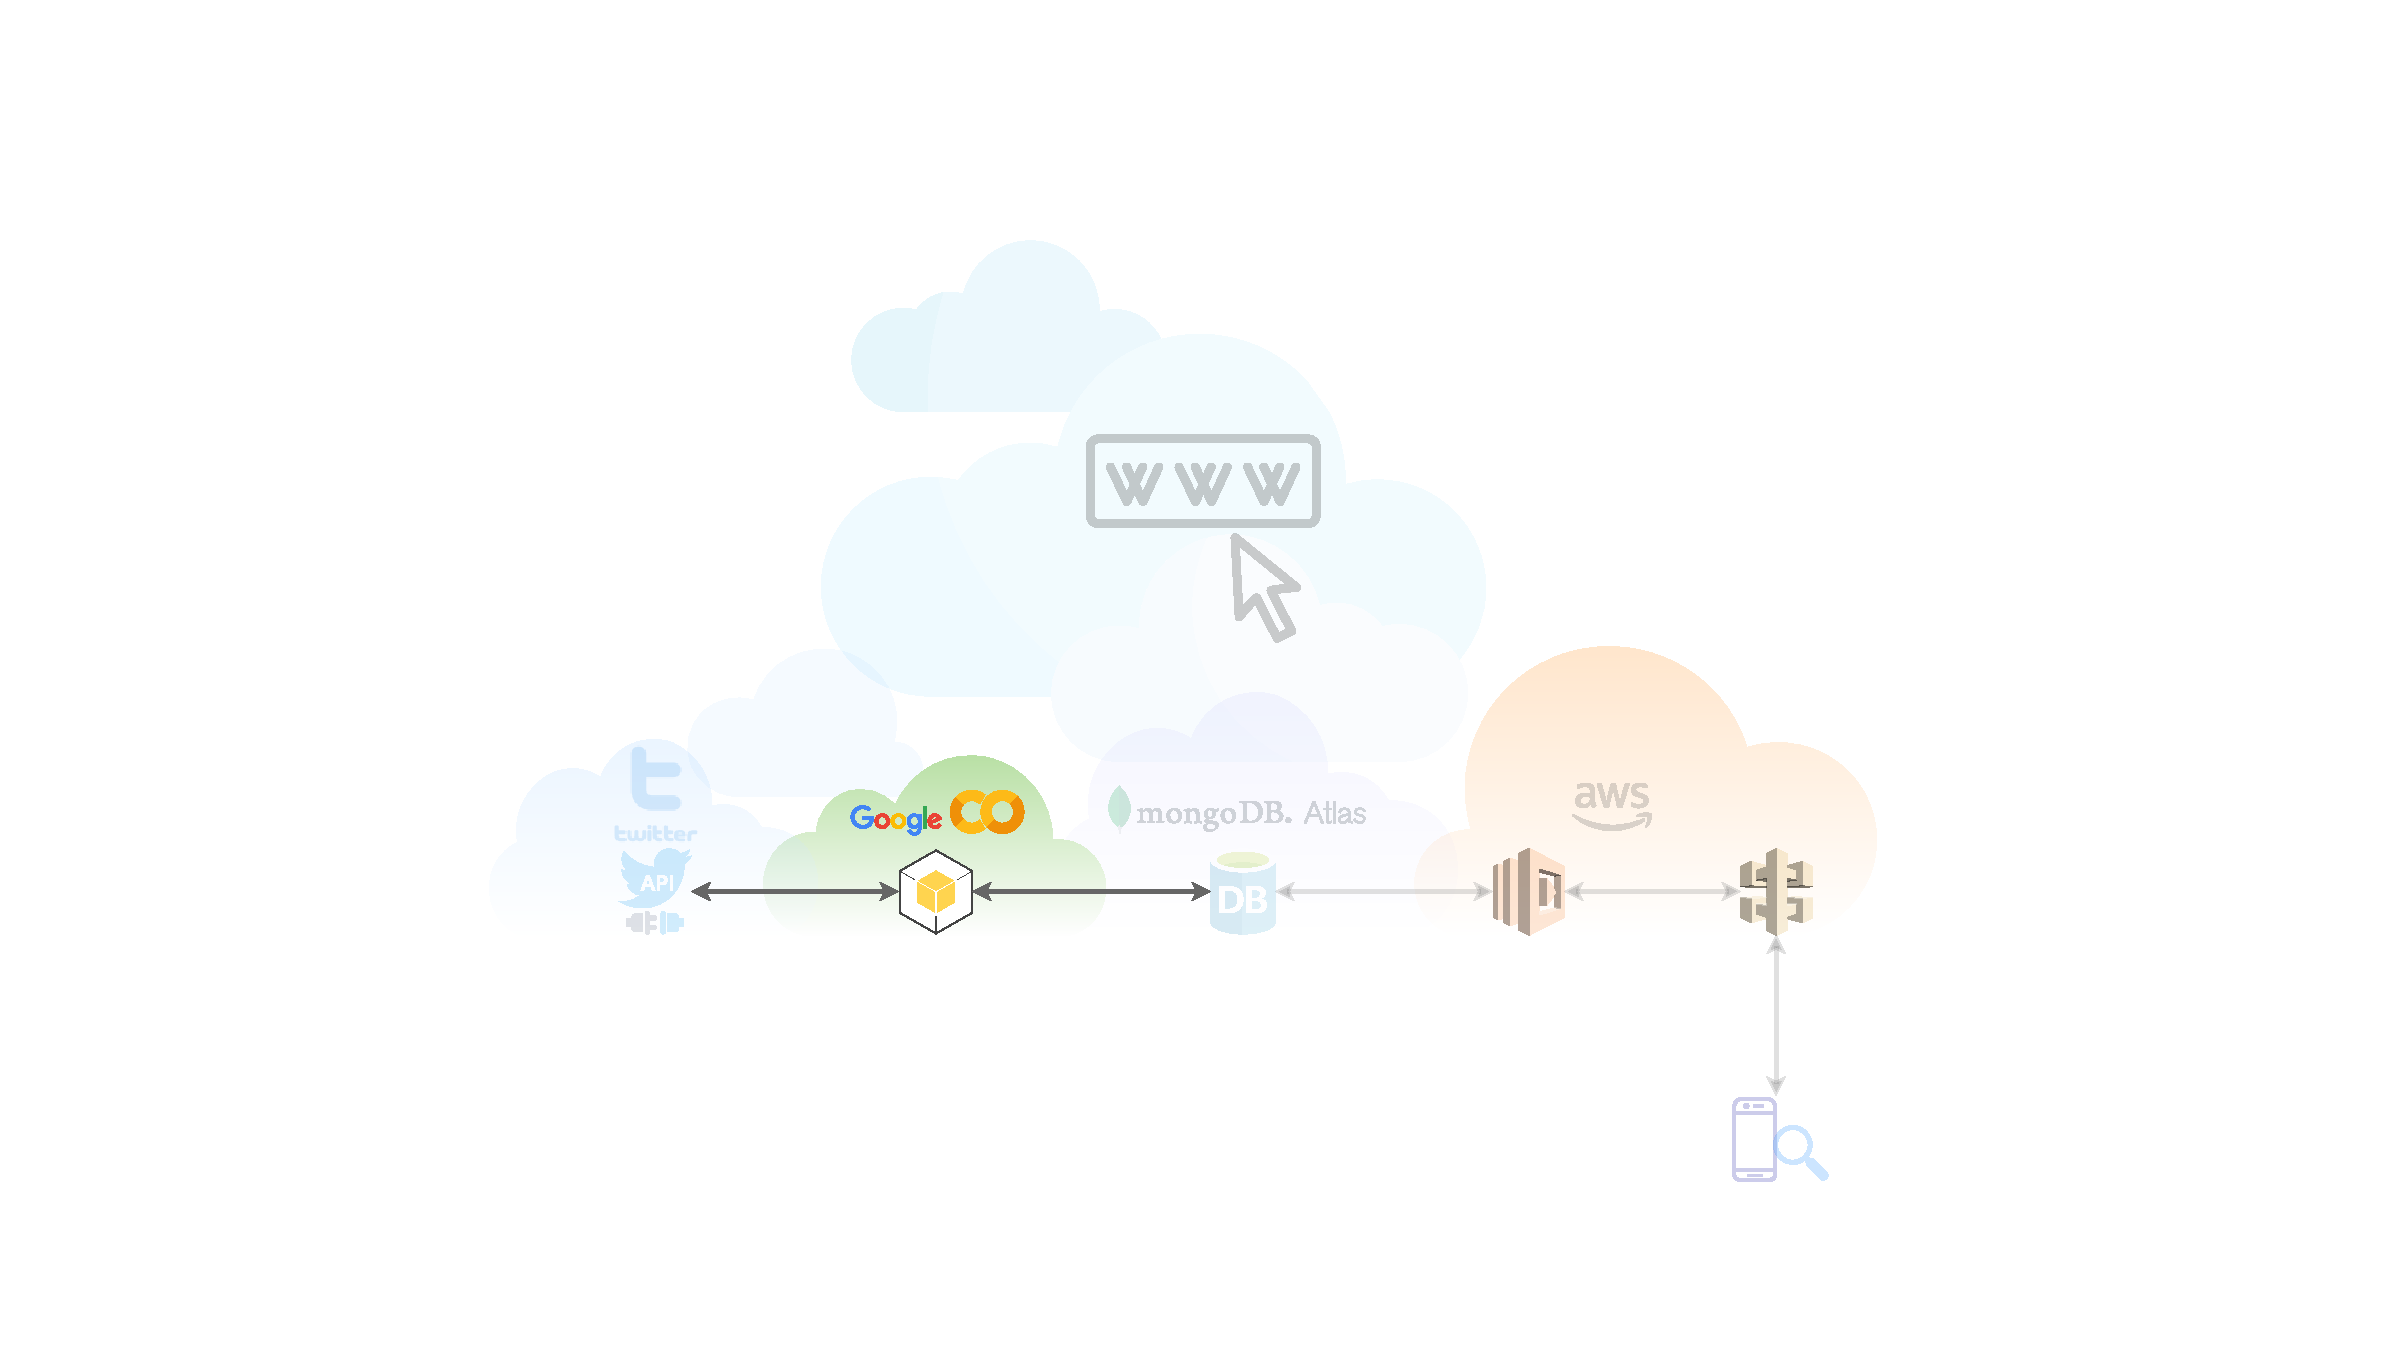
\includegraphics[width=1\paperwidth,height=1\paperheight,keepaspectratio]{Architectura_progetto_Google_Colab.pdf}
        }
    \end{figure}
\end{frame}

\subsubsection{Google Colab Python Notebook}

\begin{frame}{Installazione e importazione delle librerie}
    \fontsize{9pt}{9}\selectfont
    \begin{columns}[t]
        \column{.31\textwidth}
        dnspython è un DNS toolkit per Python.\\~\\~\\~\\~\\
        
        pymongo si usa per accedere a MongoDB.\\~\\~\\~\\~\\
        
        twitter si usa per accedere alle APIs di Twitter.
        \column{.64\textwidth}
        \vspace*{-32pt}
        \begin{figure}[H]
            \centering
            \noindent\makebox[\textheight]{
                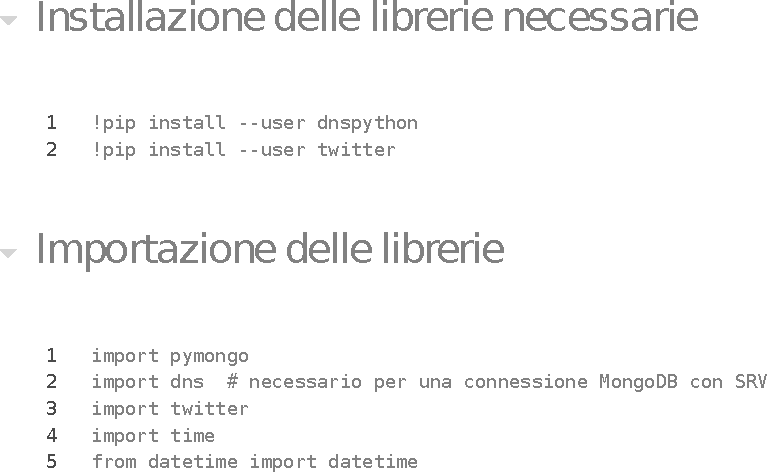
\includegraphics[width=0.5\paperwidth,height=0.5\paperheight,keepaspectratio]{Google_Colab_Python_Script_Librerie.pdf}
            }
        \end{figure}
    \end{columns}
\end{frame}

%------------------------------------------------

\subsubsection{Configurazioni per la connessione a MongoDB e a API di Twitter}

\begin{frame}{Configurazione chiavi per la connessione al MongoDB}
    \begin{columns}[t]
        \column{.31\textwidth}
        
        \column{.64\textwidth}
        \vspace*{-32pt}
        \begin{figure}[H]
            \centering
            \noindent\makebox[\textheight]{
                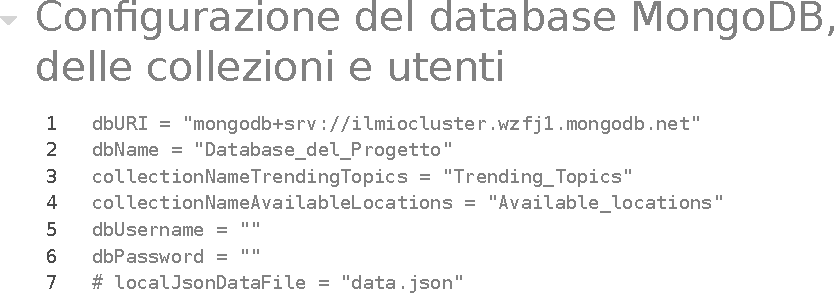
\includegraphics[width=0.5\paperwidth,height=0.5\paperheight,keepaspectratio]{Google_Colab_Python_Script_Database_NoPass.pdf}
            }
        \end{figure}
    \end{columns}
\end{frame}

%------------------------------------------------

\begin{frame}{Configurazione chiavi per la connessione al Twitter API}
    \begin{columns}[t]
        \column{.31\textwidth}
        
        \column{.64\textwidth}
        \vspace*{-32pt}
        \begin{figure}[H]
            \centering
            \noindent\makebox[\textheight]{
                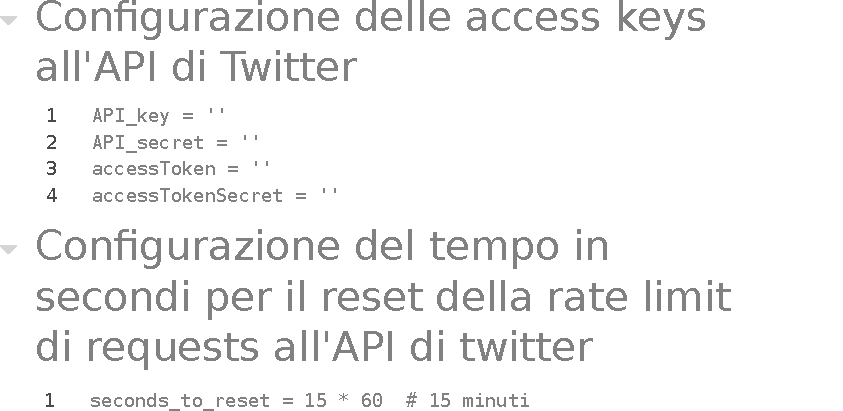
\includegraphics[width=0.5\paperwidth,height=0.5\paperheight,keepaspectratio]{Google_Colab_Python_Script_Twitter_NoPass.pdf}
            }
        \end{figure}
    \end{columns}
\end{frame}

%------------------------------------------------

\subsubsection{Procedure dello script}

\begin{frame}{Funzioni di connessione, pulizia di una collection, rinomina e stampa}
    \begin{columns}[t]
        \column{.31\textwidth}
        
        \column{.64\textwidth}
        \vspace*{-32pt}
        \begin{figure}[H]
            \centering
            \noindent\makebox[\textheight]{
                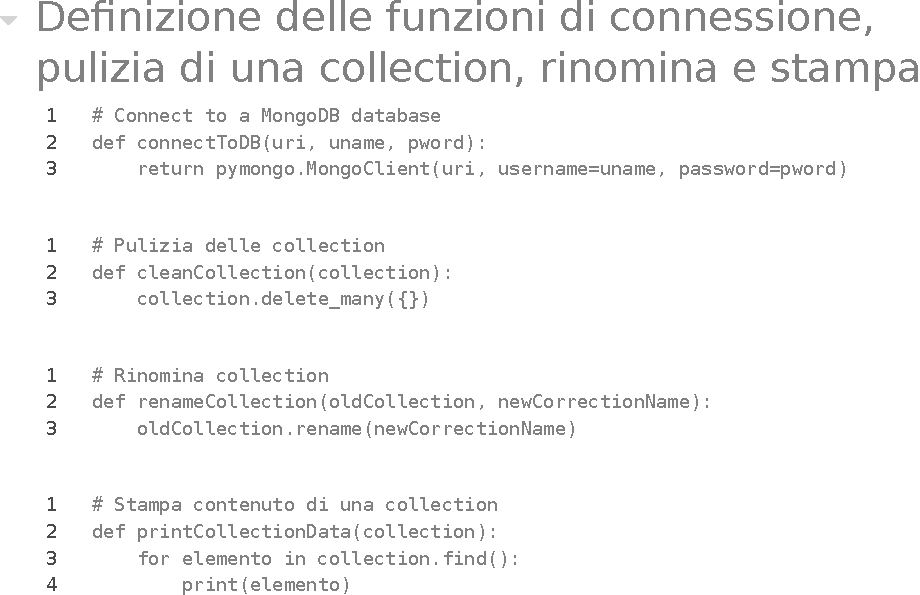
\includegraphics[width=0.67\paperwidth,height=0.67\paperheight,keepaspectratio]{Google_Colab_Python_Script_Funzioni_Connessione_Pulizia.pdf}
            }
        \end{figure}
    \end{columns}
\end{frame}

%------------------------------------------------

\begin{frame}{Funzione di controllo di duplicati, voci già presenti}
    \begin{columns}[t]
        \column{.30\textwidth}
        Controlla se un certo trend di una data in una location è già presente in database (per evitare duplicati quando lo script Python si esegue più volte al giorno).
        
        \column{.64\textwidth}
        \vspace*{-32pt}
        \begin{figure}[H]
            \centering
            \noindent\makebox[\textheight]{
                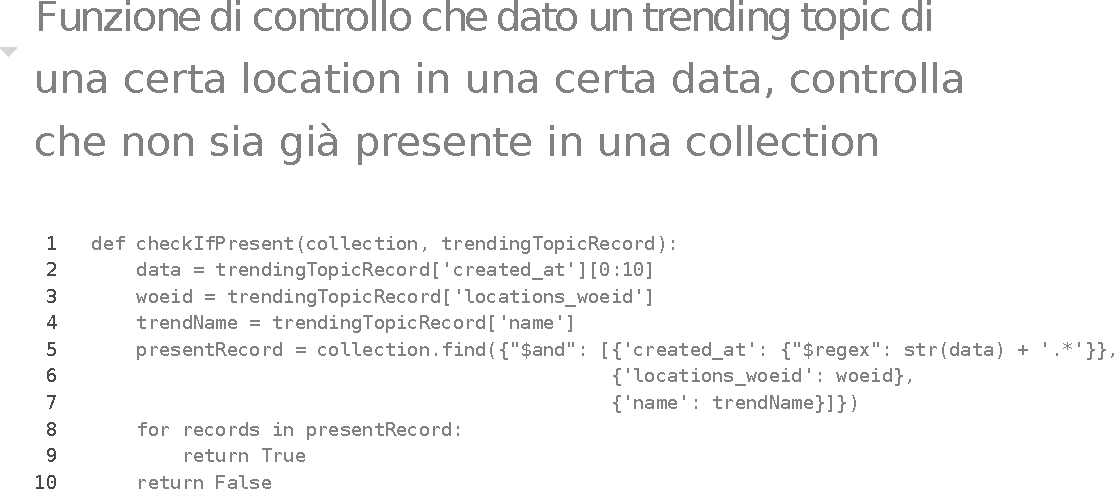
\includegraphics[width=0.64\paperwidth,height=0.64\paperheight,keepaspectratio]{Google_Colab_Python_Script_Controllo_duplicato.pdf}
            }
        \end{figure}
    \end{columns}
\end{frame}

%------------------------------------------------

\subsubsection{Gestione dei limiti del request rate}

\begin{frame}{Funzione di inserimento dei trends e gestione del rate limit}
    \begin{columns}[t]
        \column{.31\textwidth}
        
        \column{.64\textwidth}
        \vspace*{-32pt}
        \begin{figure}[H]
            \centering
            \noindent\makebox[\textheight]{
                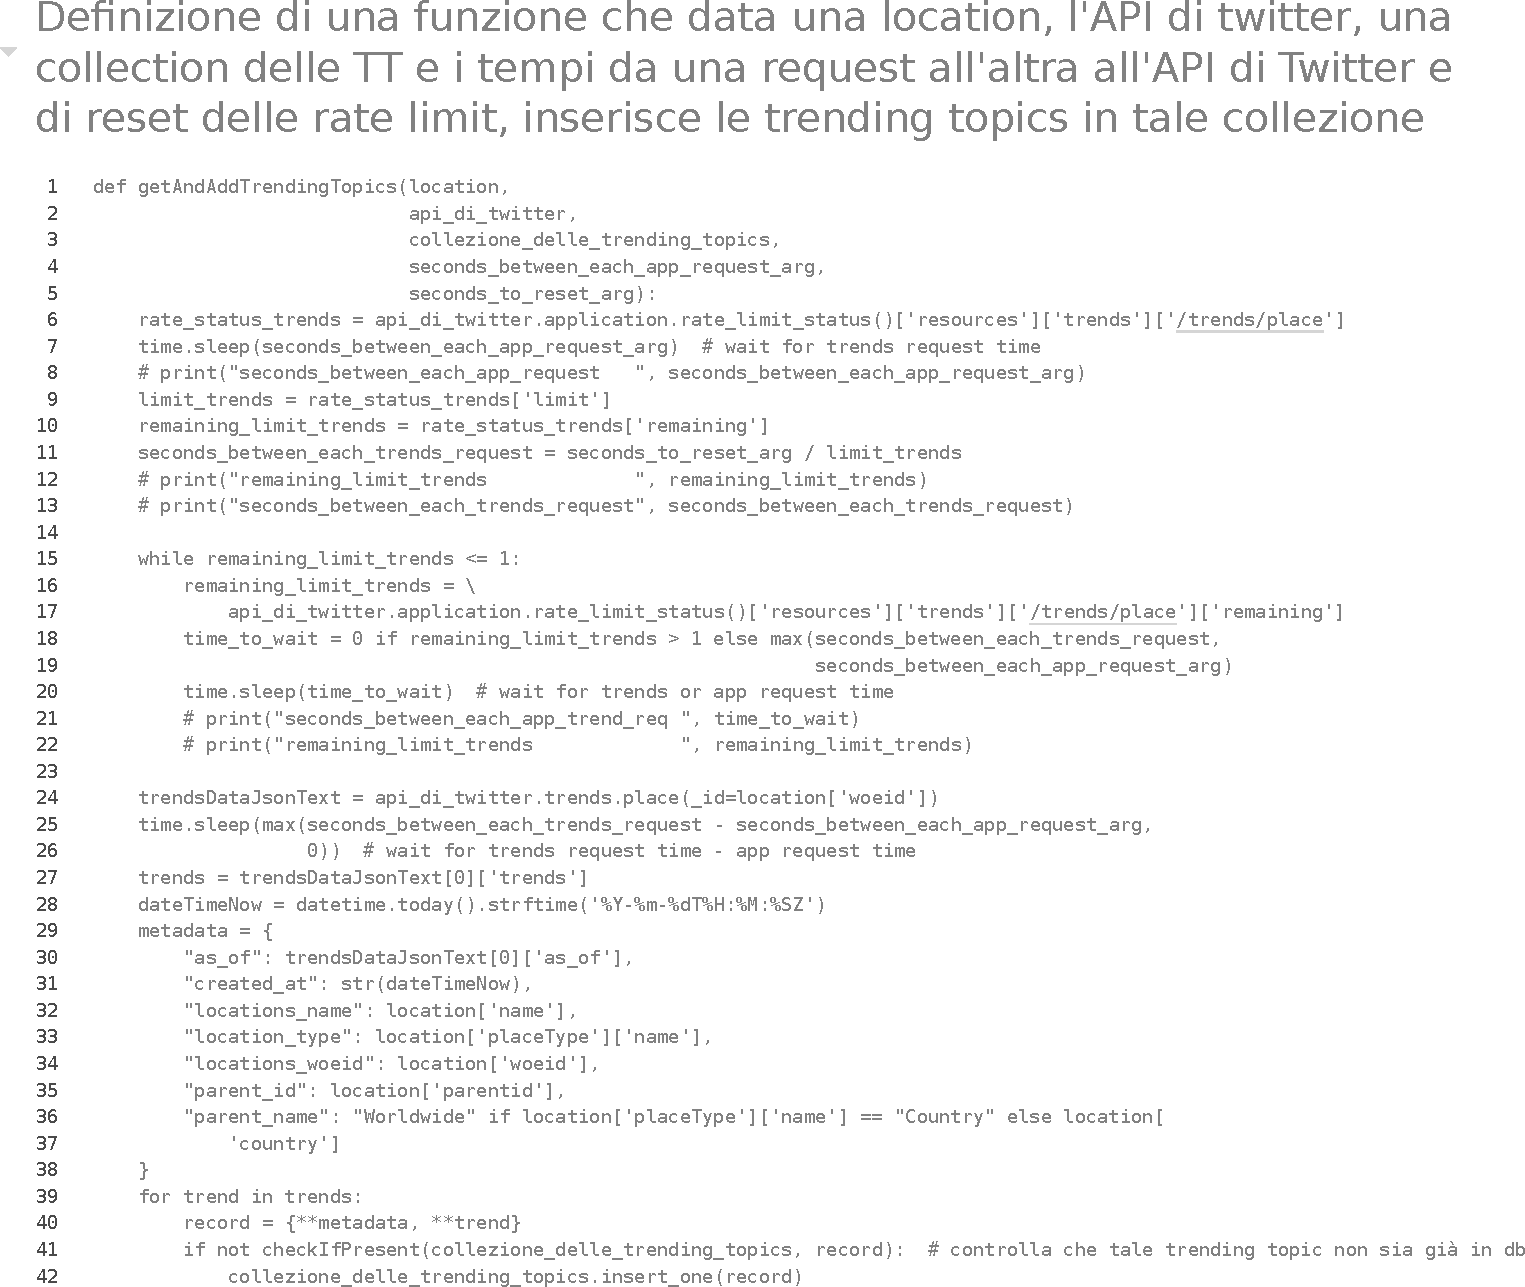
\includegraphics[width=0.64\paperwidth,height=0.75\paperheight,keepaspectratio]{Google_Colab_Python_Script_Funzione_Inserimento_Trends.pdf}
            }
        \end{figure}
    \end{columns}
\end{frame}

%------------------------------------------------

\subsubsection{Funzione di inserimento delle available locations e esecuzione delle operazioni}

\begin{frame}{Funzione di inserimento delle available locations (1)}
    \begin{columns}[t]
        \column{.31\textwidth}
        Continua nella slide dopo...
        
        \column{.64\textwidth}
        \vspace*{-32pt}
        \begin{figure}[H]
            \centering
            \noindent\makebox[\textheight]{
                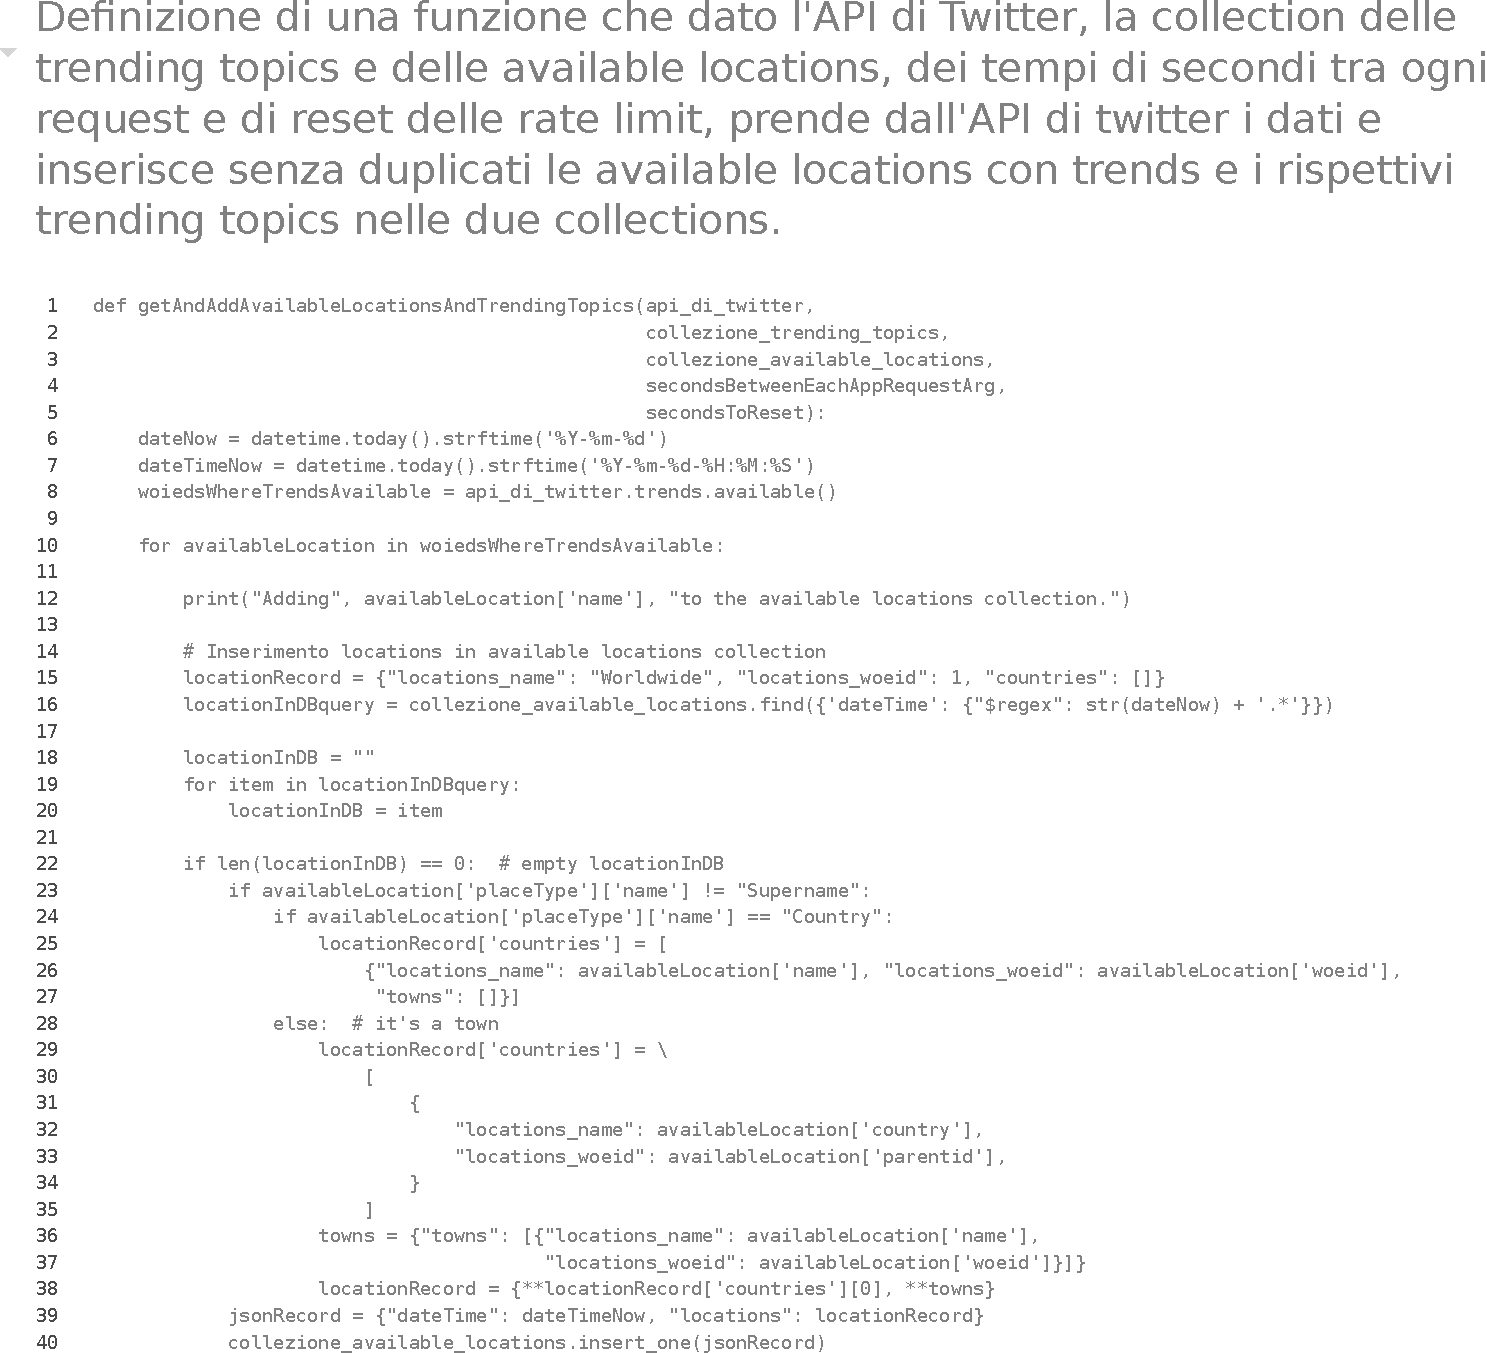
\includegraphics[width=0.64\paperwidth,height=0.75\paperheight,keepaspectratio]{Google_Colab_Python_Script_Funzione_Inserimento_Available_Locations_1.pdf}
            }
        \end{figure}
    \end{columns}
\end{frame}

%------------------------------------------------

\begin{frame}{Funzione di inserimento delle available locations (2)}
    \begin{columns}[t]
        \column{.31\textwidth}
        
        \column{.64\textwidth}
        \vspace*{-32pt}
        \begin{figure}[H]
            \centering
            \noindent\makebox[\textheight]{
                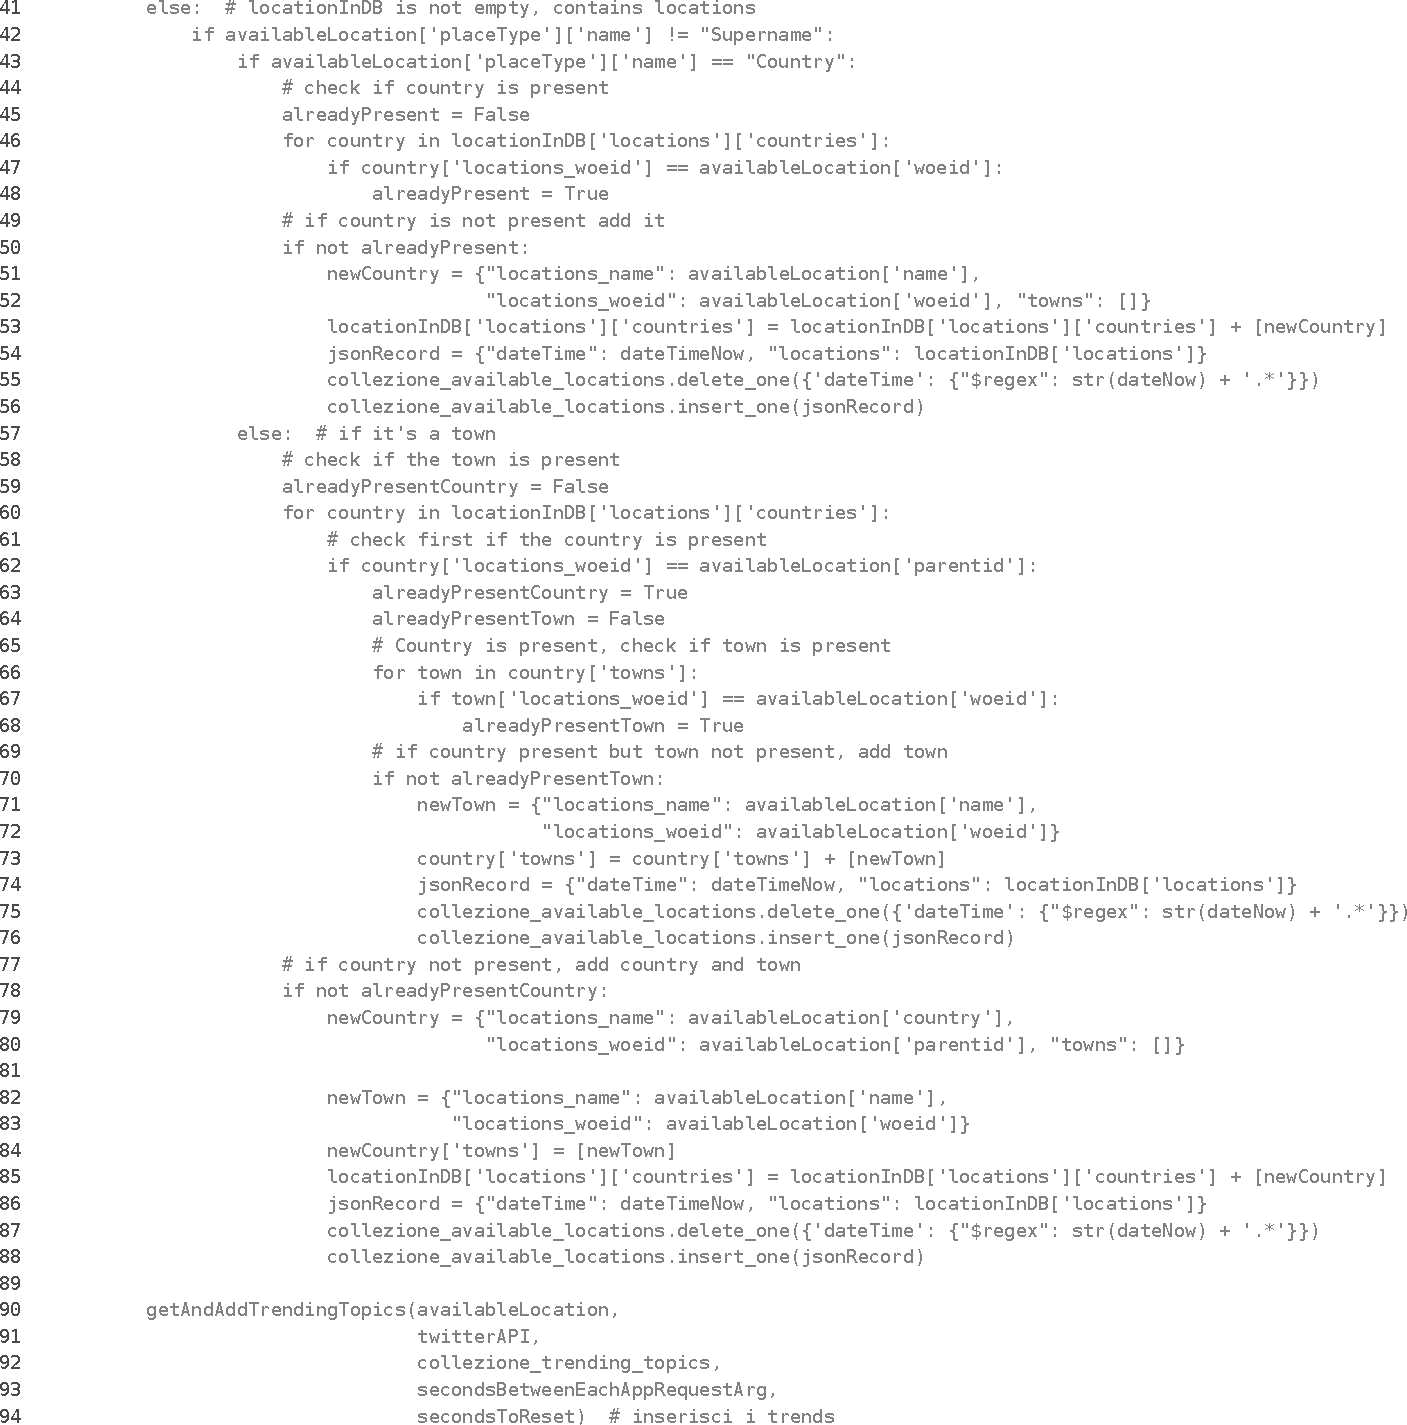
\includegraphics[width=0.64\paperwidth,height=0.75\paperheight,keepaspectratio]{Google_Colab_Python_Script_Funzione_Inserimento_Available_Locations_2.pdf}
            }
        \end{figure}
    \end{columns}
\end{frame}

%------------------------------------------------

\begin{frame}{Esecuzione delle operazioni}
    \begin{columns}[t]
        \column{.31\textwidth}
        Il 'main' dove si chiamano le funzioni definite precedentemente
        
        \column{.64\textwidth}
        \vspace*{-32pt}
        \begin{figure}[H]
            \centering
            \noindent\makebox[\textheight]{
                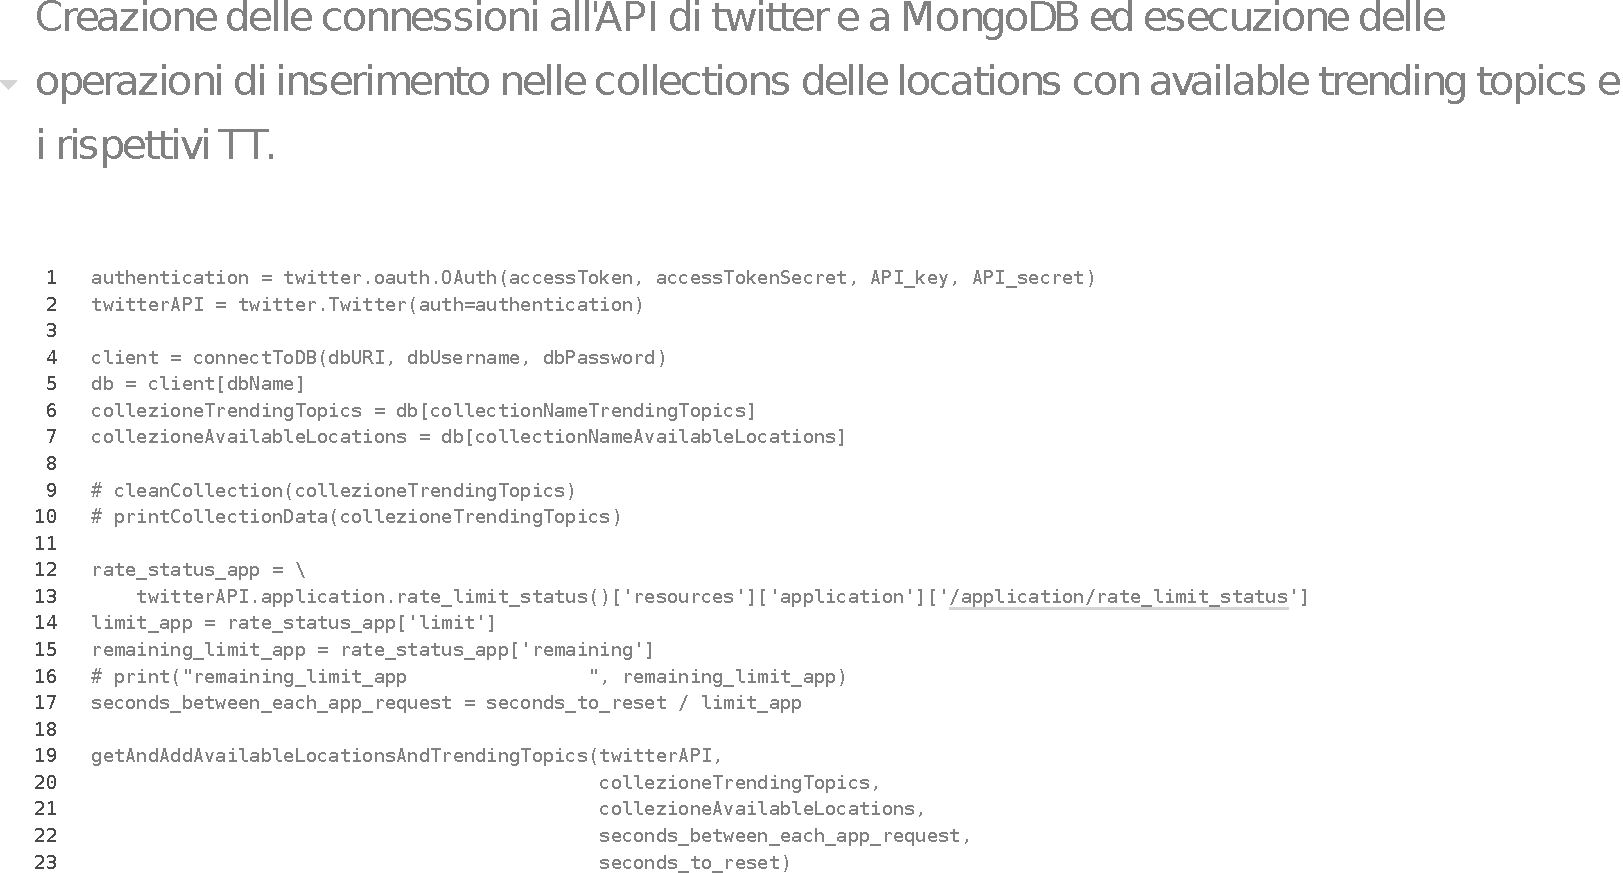
\includegraphics[width=0.5\paperwidth,height=0.5\paperheight,keepaspectratio]{Google_Colab_Python_Script_Esecuzione_delle_operazioni.pdf}
            }
        \end{figure}
    \end{columns}
\end{frame}

%------------------------------------------------

\subsection{AWS Cloud per API e funzioni}

\begin{frame}{AWS Cloud Platform}
    \vspace*{-56pt}
    \begin{figure}[H]
        \centering
        \noindent\makebox[\textheight]{
            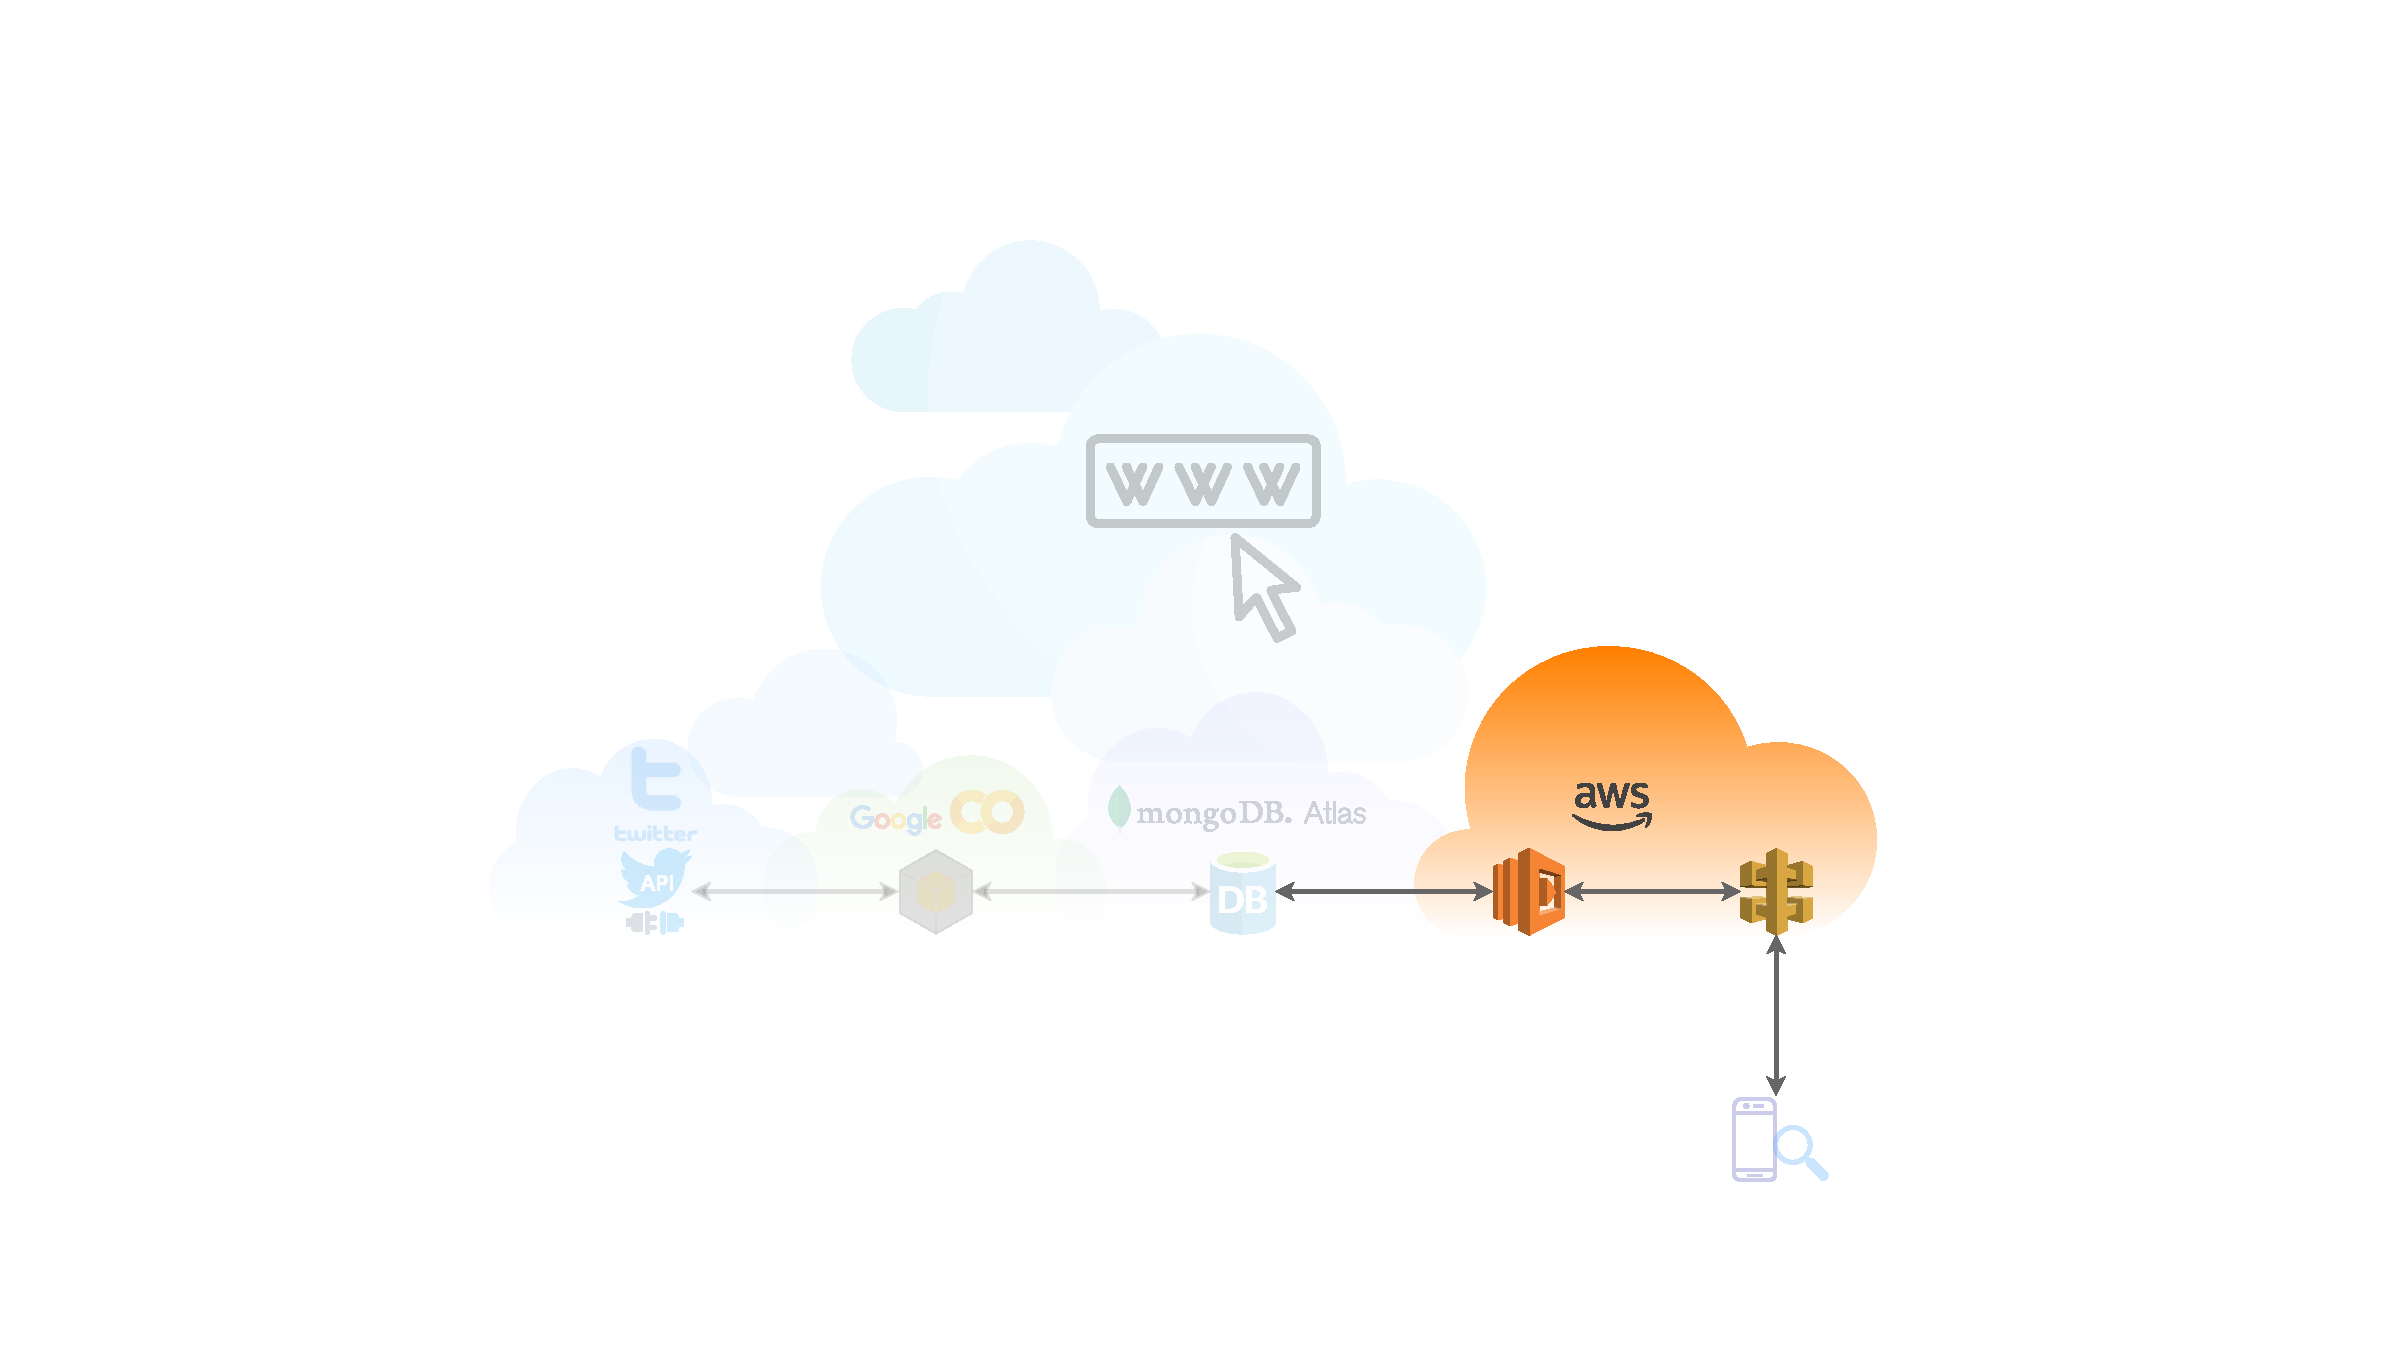
\includegraphics[width=1\paperwidth,height=1\paperheight,keepaspectratio]{Architectura_progetto_AWS.pdf}
        }
    \end{figure}
\end{frame}

%------------------------------------------------

\subsubsection{AWS API Gateway - Trends\_API}

\begin{frame}{AWS API Gateway - Trends\_API}
    \vspace*{-56pt}
    \begin{figure}[H]
        \centering
        \noindent\makebox[\textheight]{
            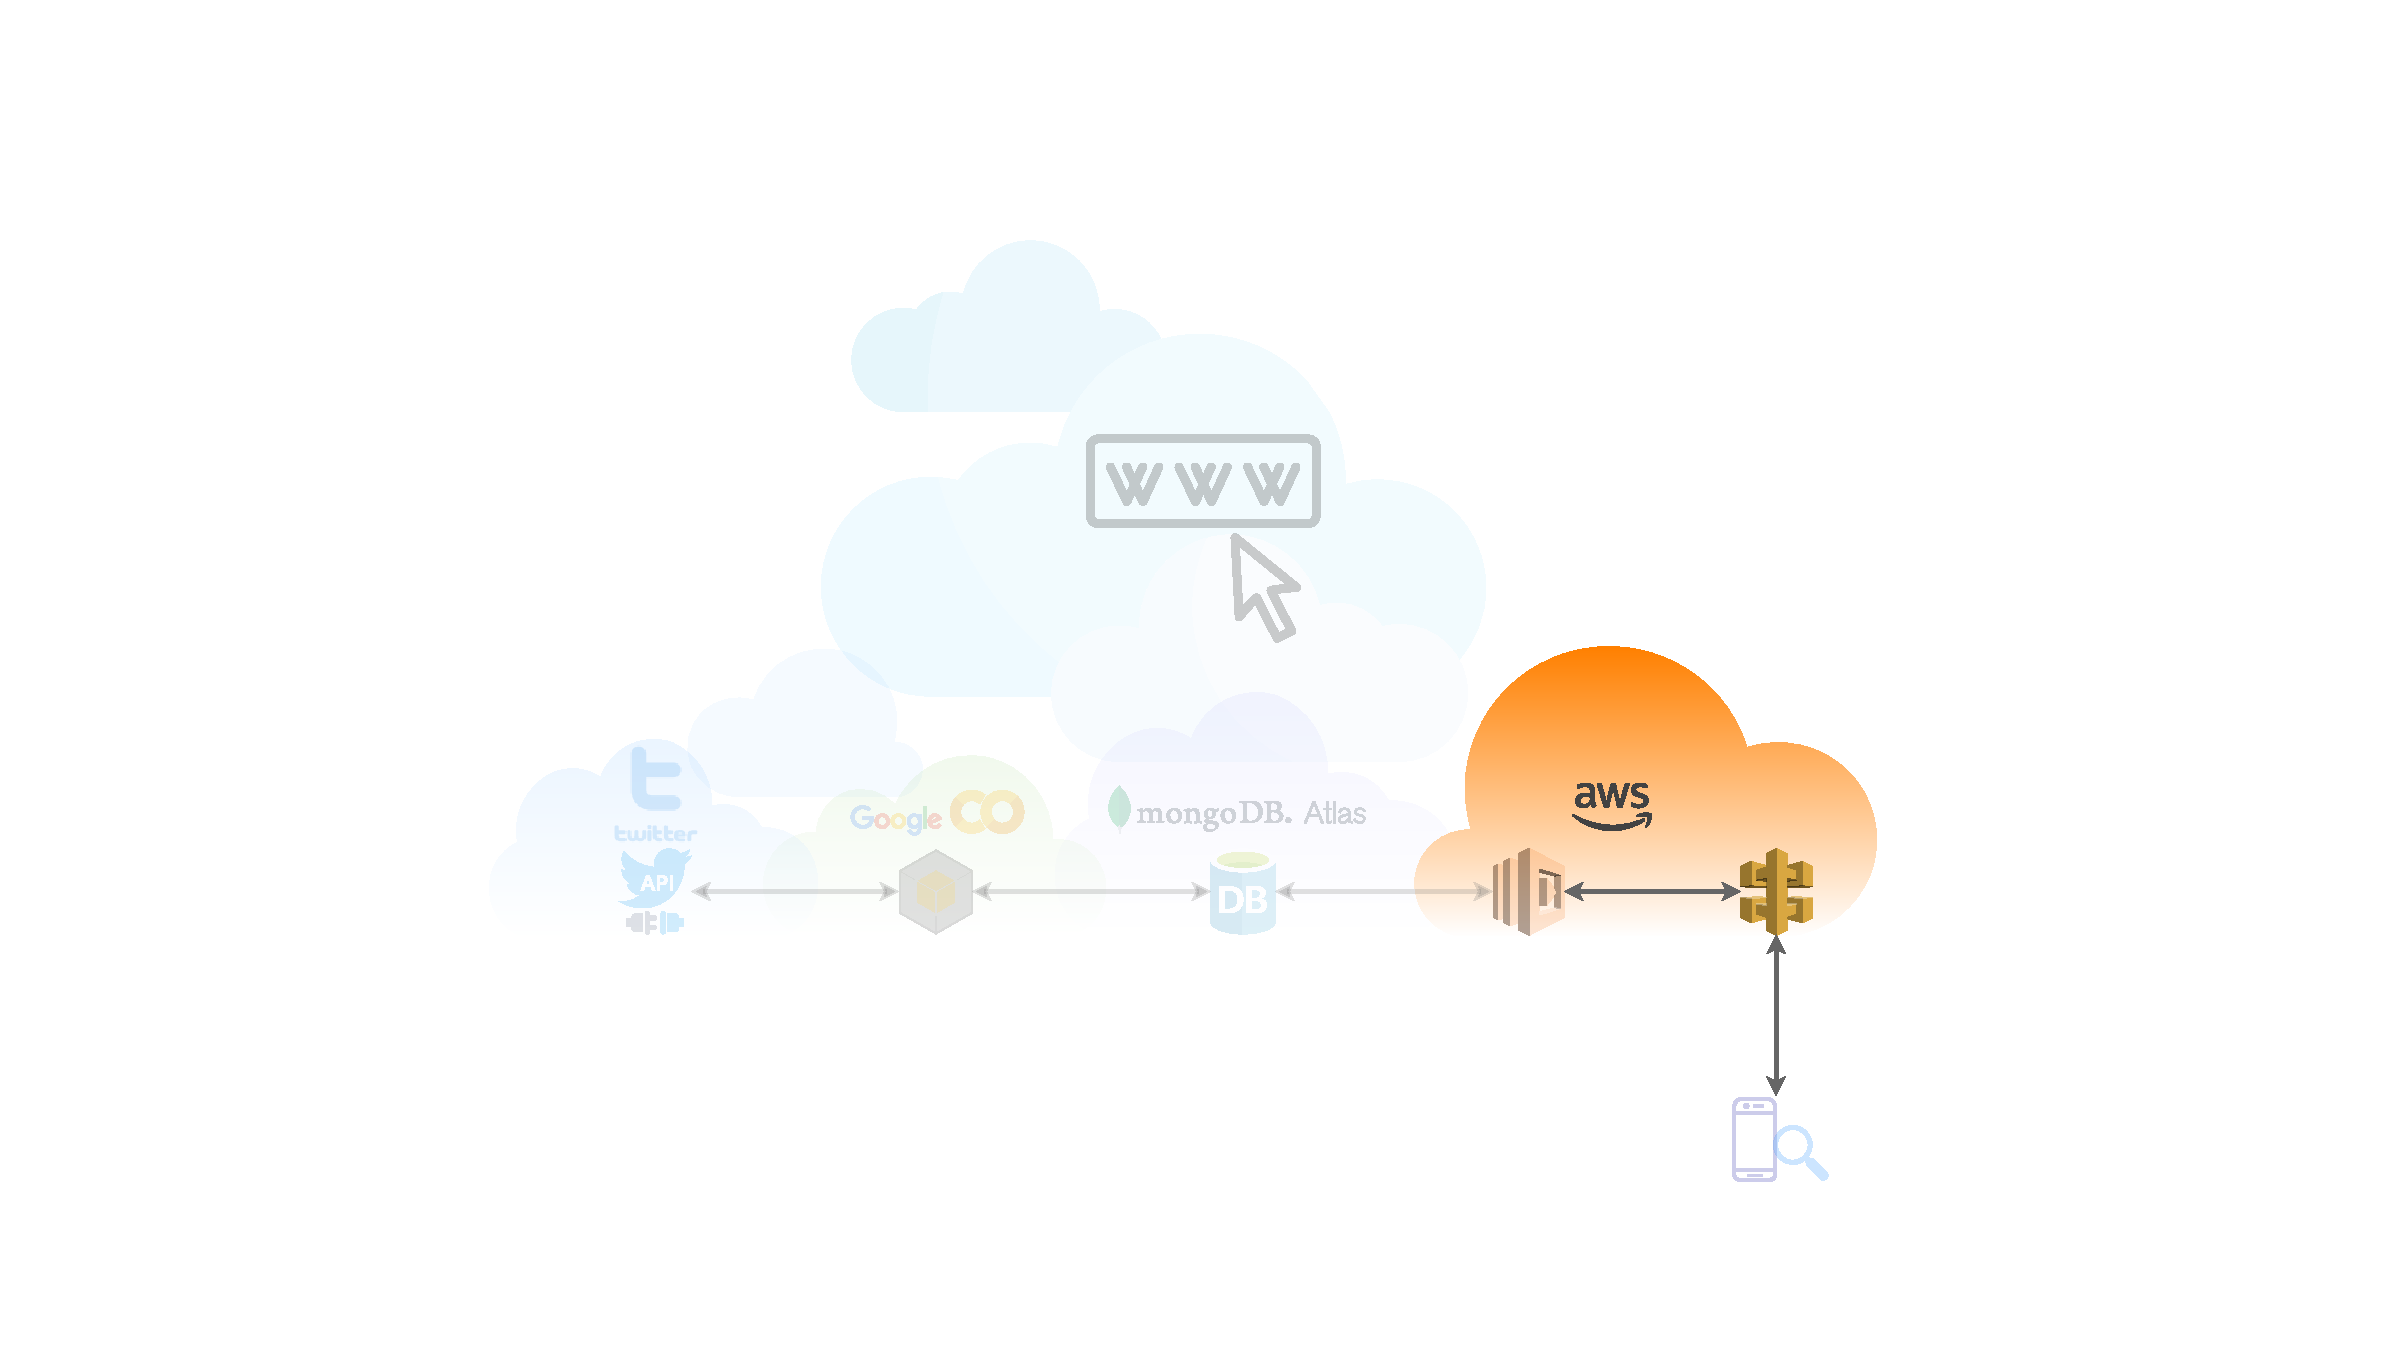
\includegraphics[width=1\paperwidth,height=1\paperheight,keepaspectratio]{Architectura_progetto_AWS_API.pdf}
        }
    \end{figure}
\end{frame}

%------------------------------------------------

\begin{frame}
    \begin{figure}[H]
        \centering
        \noindent\makebox[\textheight]{
            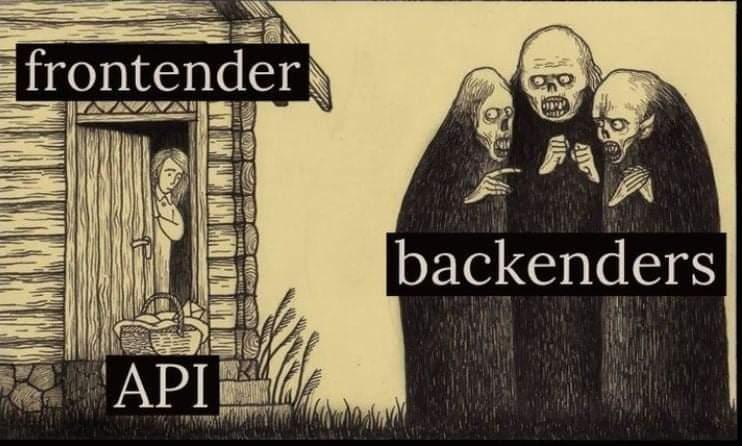
\includegraphics[width=0.8\paperwidth,height=0.8\paperheight,keepaspectratio]{Meme_Frontender_Backenders_API.jpg}
        }
    \end{figure}
\end{frame}

%------------------------------------------------

\begin{frame}{AWS API Gateway - Trends\_API/locations}
    \fontsize{10pt}{10}\selectfont
    \begin{columns}[t]
        \column{.2\textwidth}
        Per richiedere le locations con trends in una certa data, l'unico parametro è la data.\\~\\~\\~\\~\\
        
        Le richieste e le risposte vengono gestite dalla AWS Lambda Function 'getAvailableLocationsByDate'.
        \column{.75\textwidth}
        \vspace*{-16pt}
        \begin{figure}[H]
            \centering
            \noindent\makebox[\textheight]{
                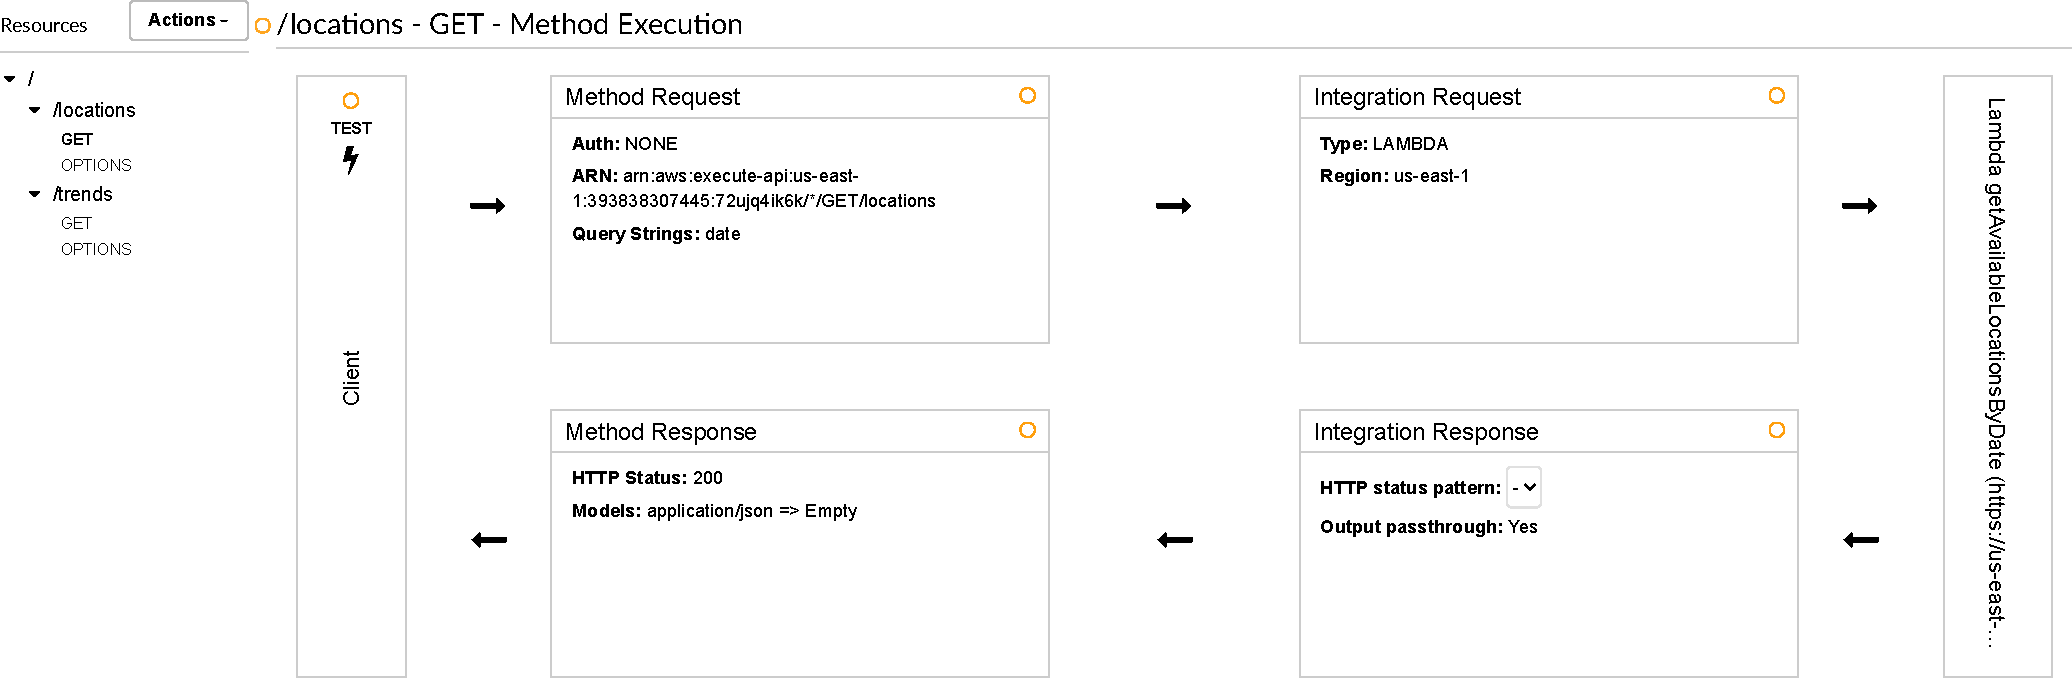
\includegraphics[width=0.75\paperwidth,height=0.75\paperheight,keepaspectratio]{AWS_API_Gateway_Locations.pdf}
            }
        \end{figure}
    \end{columns}
\end{frame}

%------------------------------------------------

\begin{frame}{AWS API Gateway - Trends\_API/trends}
    \fontsize{8pt}{8}\selectfont
    \begin{columns}[t]
        \column{.2\textwidth}
        Per richiedere le trending topics in una certa data in una certa location, i parametri richiesti sono la data e l'woeid della location.\\~\\~\\~\\~\\
        
        Inoltre per l'impaginazione lato FrontEnd serve sapere il numero della pagina e il numero di trends da inviare in risposta.\\~\\~\\~\\~\\
        
        Le richieste e le risposte vengono gestite dalla AWS Lambda Function 'getTrendsByDateAndLocation'.
        \column{.75\textwidth}
        \vspace*{-8pt}
        \begin{figure}[H]
            \centering
            \noindent\makebox[\textheight]{
                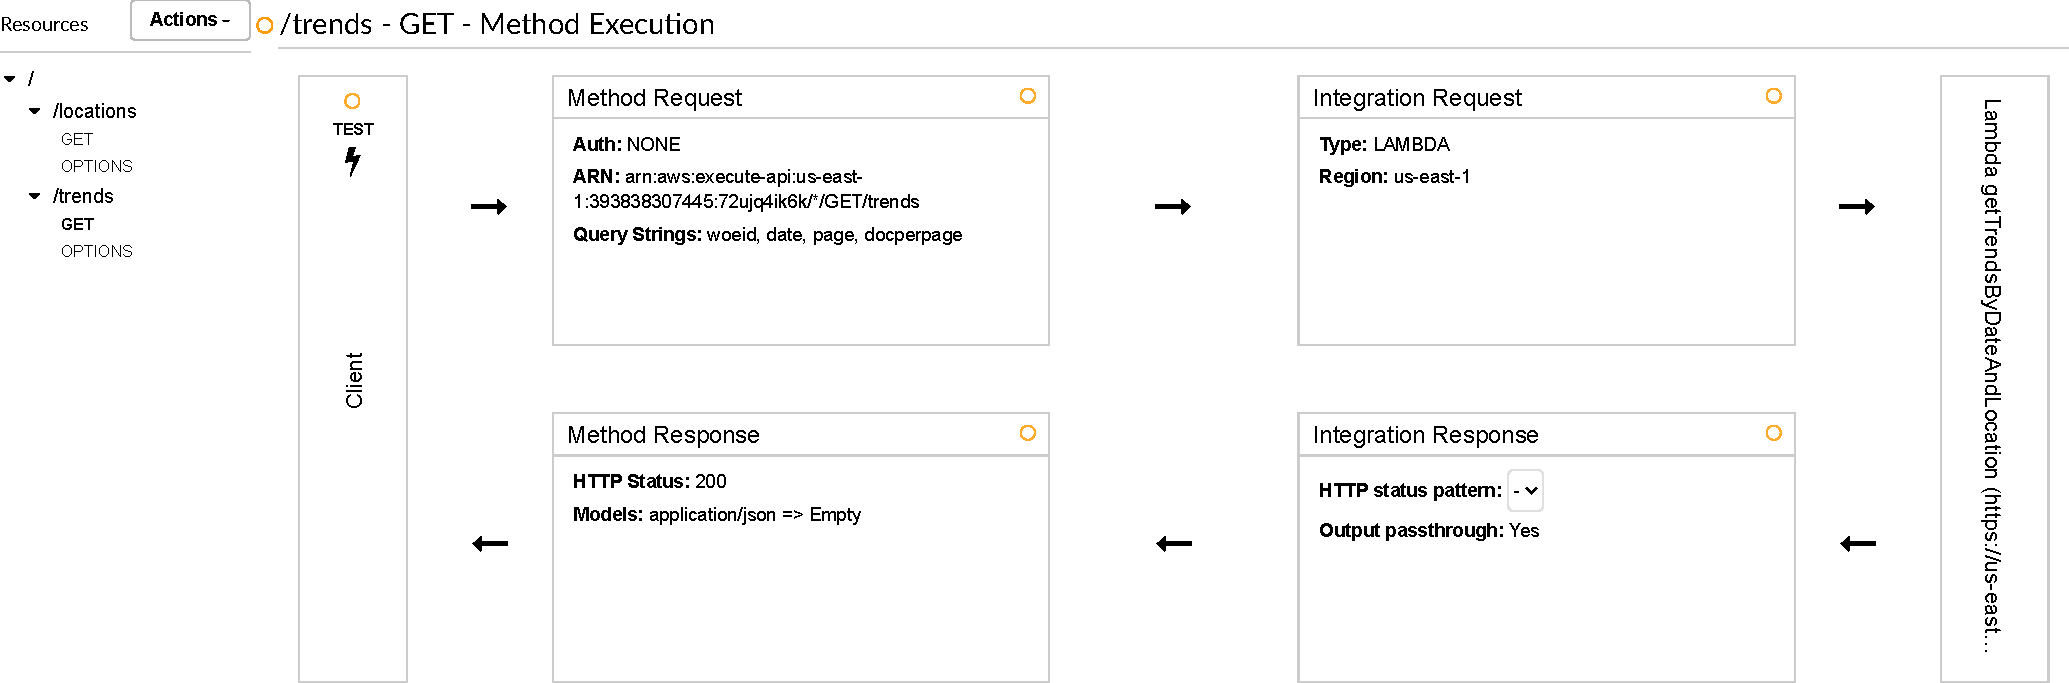
\includegraphics[width=0.75\paperwidth,height=0.75\paperheight,keepaspectratio]{AWS_API_Gateway_Trends.pdf}
            }
        \end{figure}
    \end{columns}
\end{frame}

%------------------------------------------------

\subsubsection{AWS Lambda Functions}

\begin{frame}{AWS Lambda Functions}
    \vspace*{-56pt}
    \begin{figure}[H]
        \centering
        \noindent\makebox[\textheight]{
            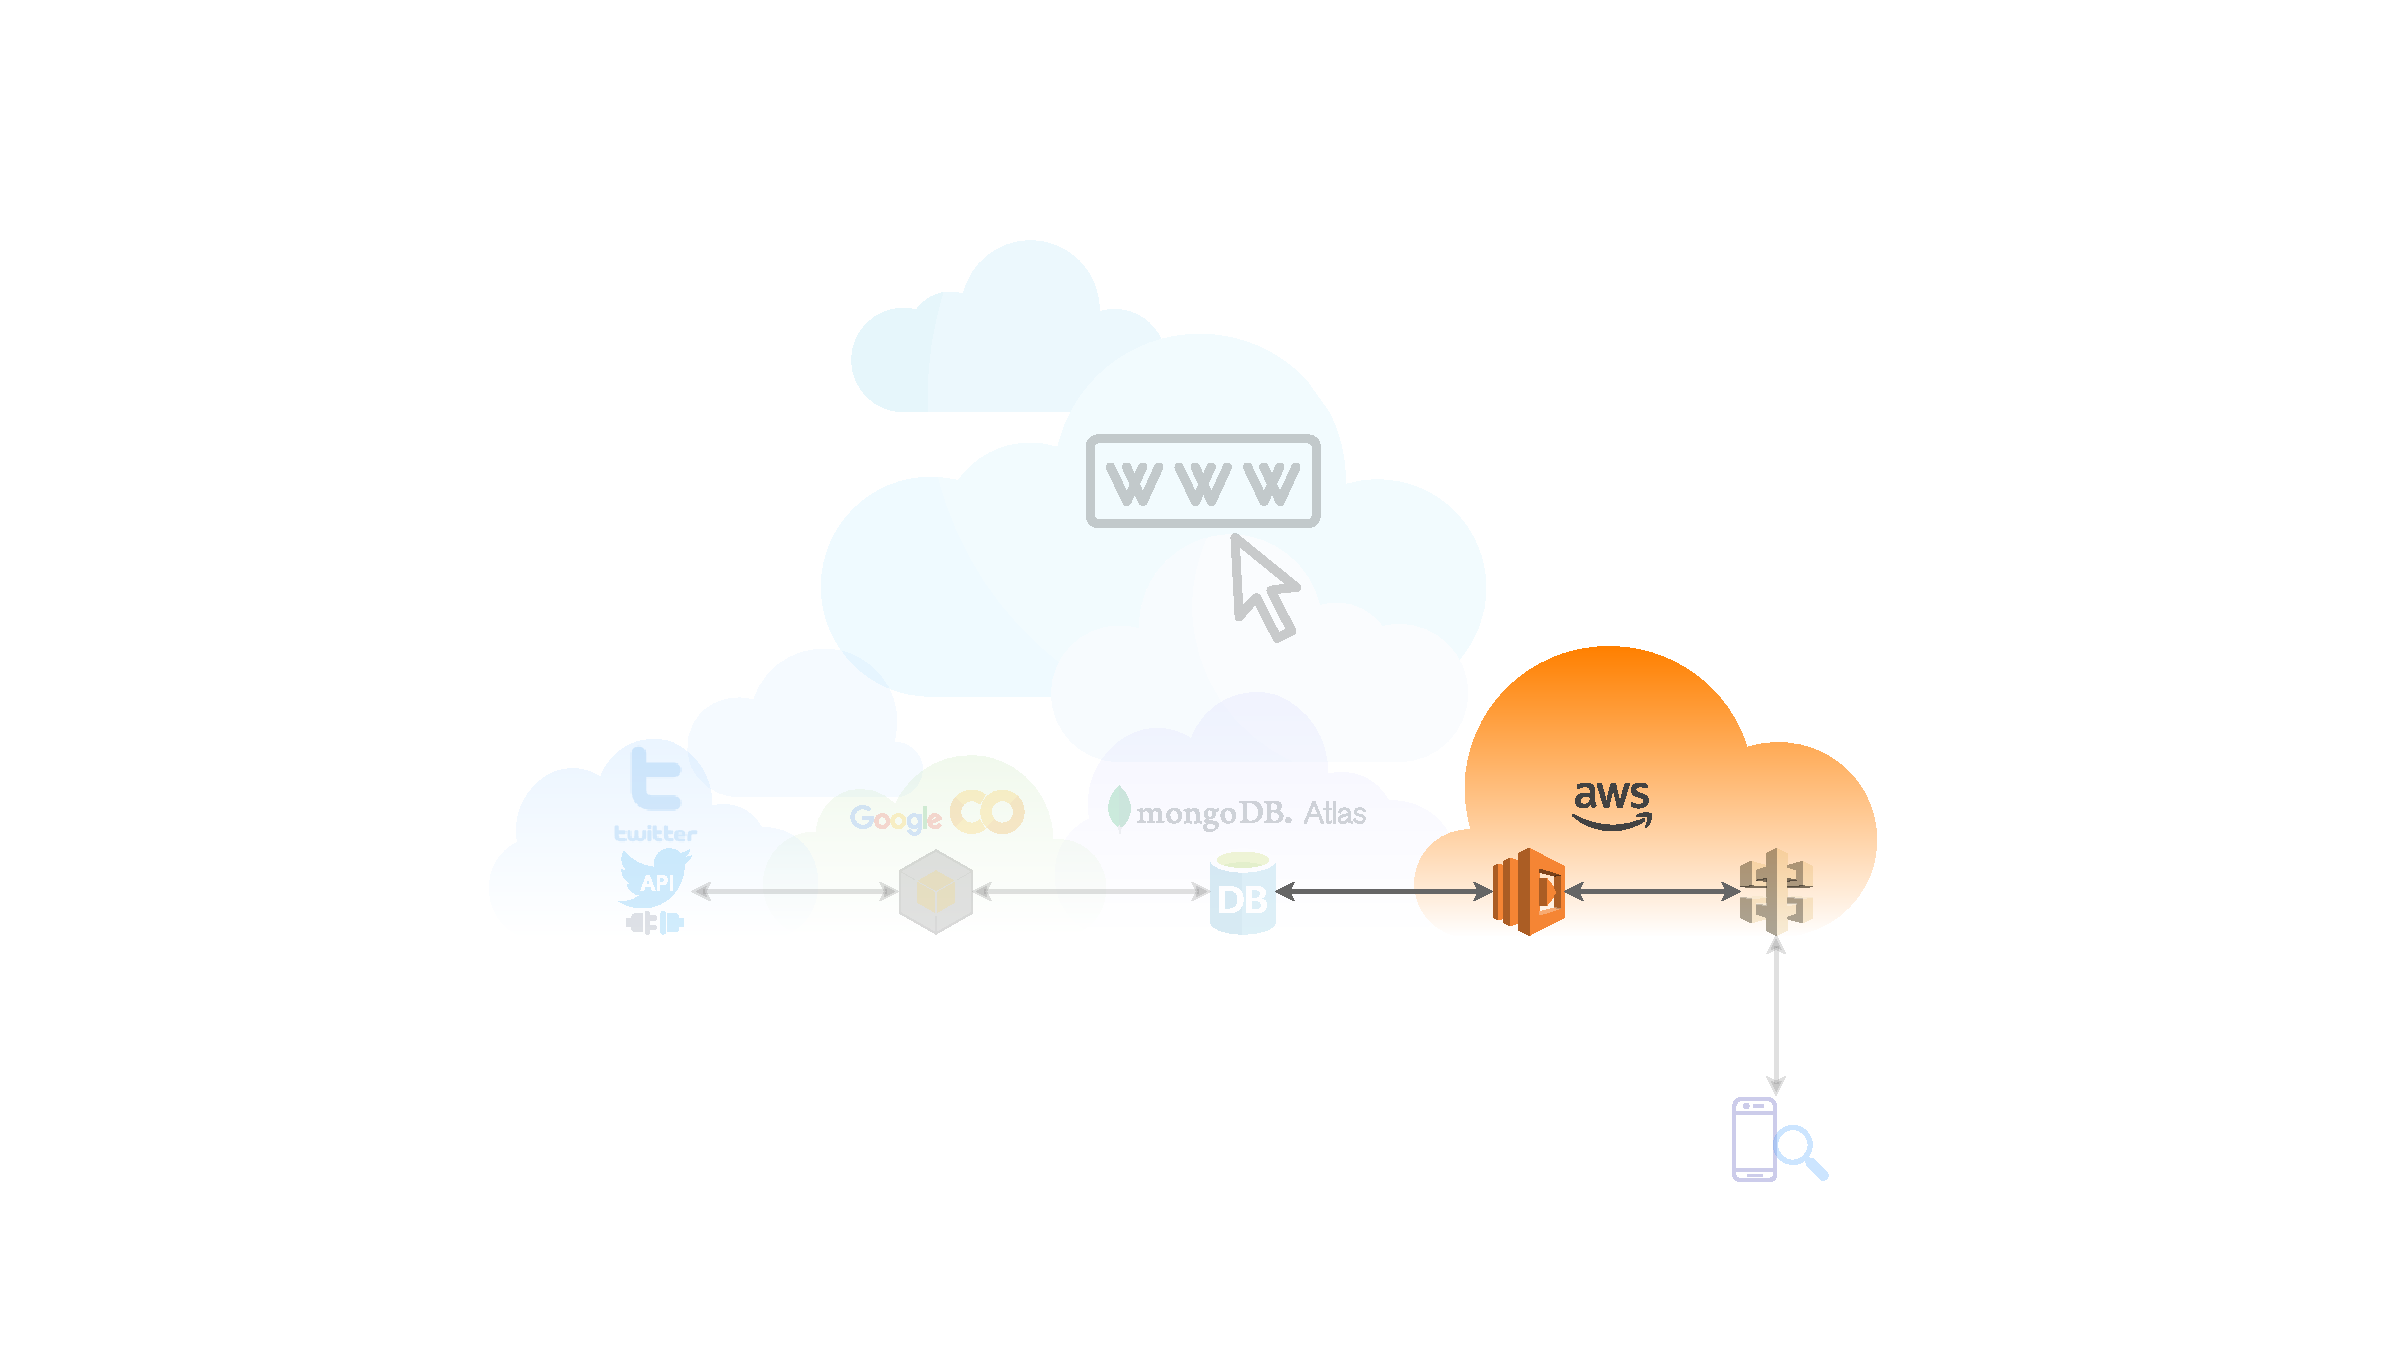
\includegraphics[width=1\paperwidth,height=1\paperheight,keepaspectratio]{Architectura_progetto_AWS_Lambda.pdf}
        }
    \end{figure}
\end{frame}

%------------------------------------------------

\begin{frame}
    \begin{figure}[H]
        \centering
        \noindent\makebox[\textheight]{
            
\includegraphics[width=0.8\paperwidth,height=0.8\paperheight,keepaspectratio]{Meme_Me_A_normal_Function_Lambda.jpg}
        }
    \end{figure}
\end{frame}

%------------------------------------------------

\begin{frame}{AWS Lambda Functions - getAvailableLocationsByDate}
    \begin{columns}[t]
        \column{.31\textwidth}
        Interroga il MongoDB database per avere le locations figlie di un elemento con data quella fornita come parametro della query all'API.\\~\\~\\~\\~\\
        
        Risponde alla richiesta dell'API.
        
        \column{.64\textwidth}
        \vspace*{-32pt}
        \begin{figure}[H]
            \centering
            \noindent\makebox[\textheight]{
                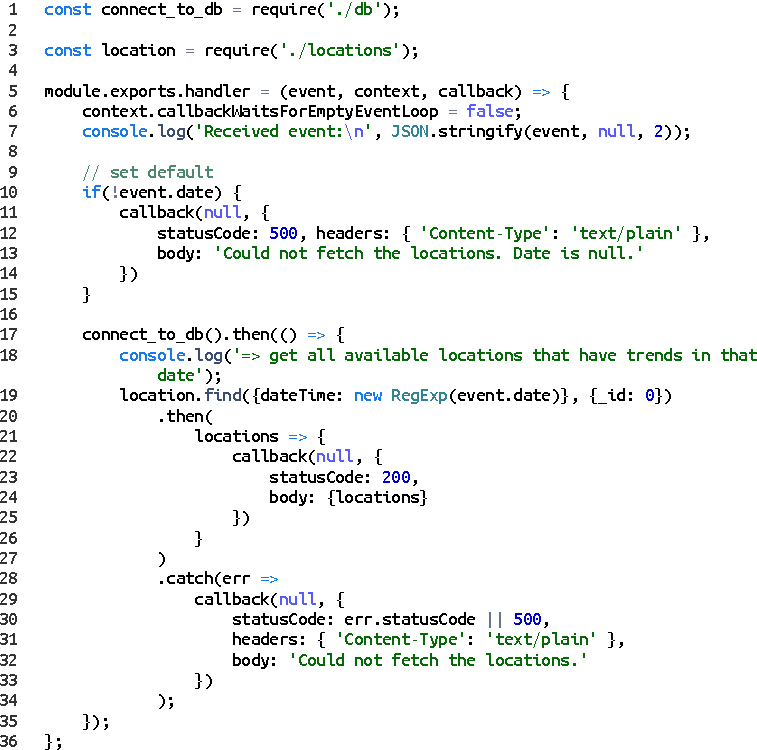
\includegraphics[width=0.64\paperwidth,height=0.64\paperheight,keepaspectratio]{AWS_Lambda_getAvailableLocationsByDate.pdf}
            }
        \end{figure}
    \end{columns}
\end{frame}

%------------------------------------------------

\begin{frame}{AWS Lambda Functions - getTrendsByDateAndLocation}
    \begin{columns}[t]
        \column{.31\textwidth}
        Interroga il MongoDB database per avere i nomi dei trends presenti con data e location fornita come parametro della query all'API.\\~\\~\\~\\~\\
        
        Risponde alla richiesta dell'API.
        
        \column{.64\textwidth}
        \vspace*{-32pt}
        \begin{figure}[H]
            \centering
            \noindent\makebox[\textheight]{
                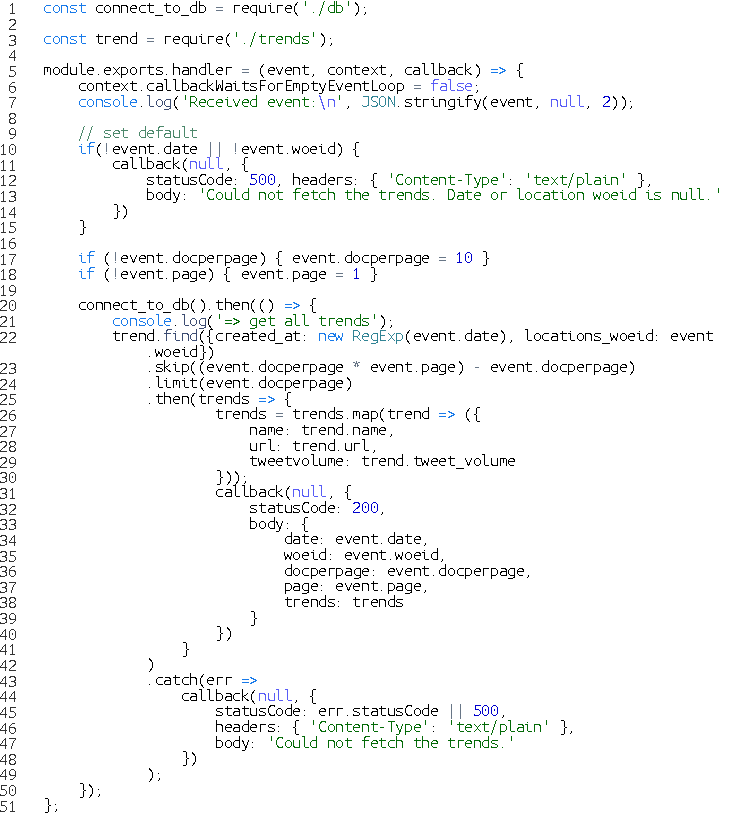
\includegraphics[width=0.75\paperwidth,height=0.75\paperheight,keepaspectratio]{AWS_Lambda_getTrendsByDateAndLocation.pdf}
            }
        \end{figure}
    \end{columns}
\end{frame}

%------------------------------------------------

\section{FrontEnd}

\begin{frame}{\secname}
    \tableofcontents[sections={\thesection}, subsubsectionstyle=show, sectionstyle=hide]
\end{frame}

%------------------------------------------------

\begin{frame}{Progressive WebApp}
    \vspace*{-56pt}
    \begin{figure}[H]
        \centering
        \noindent\makebox[\textheight]{
            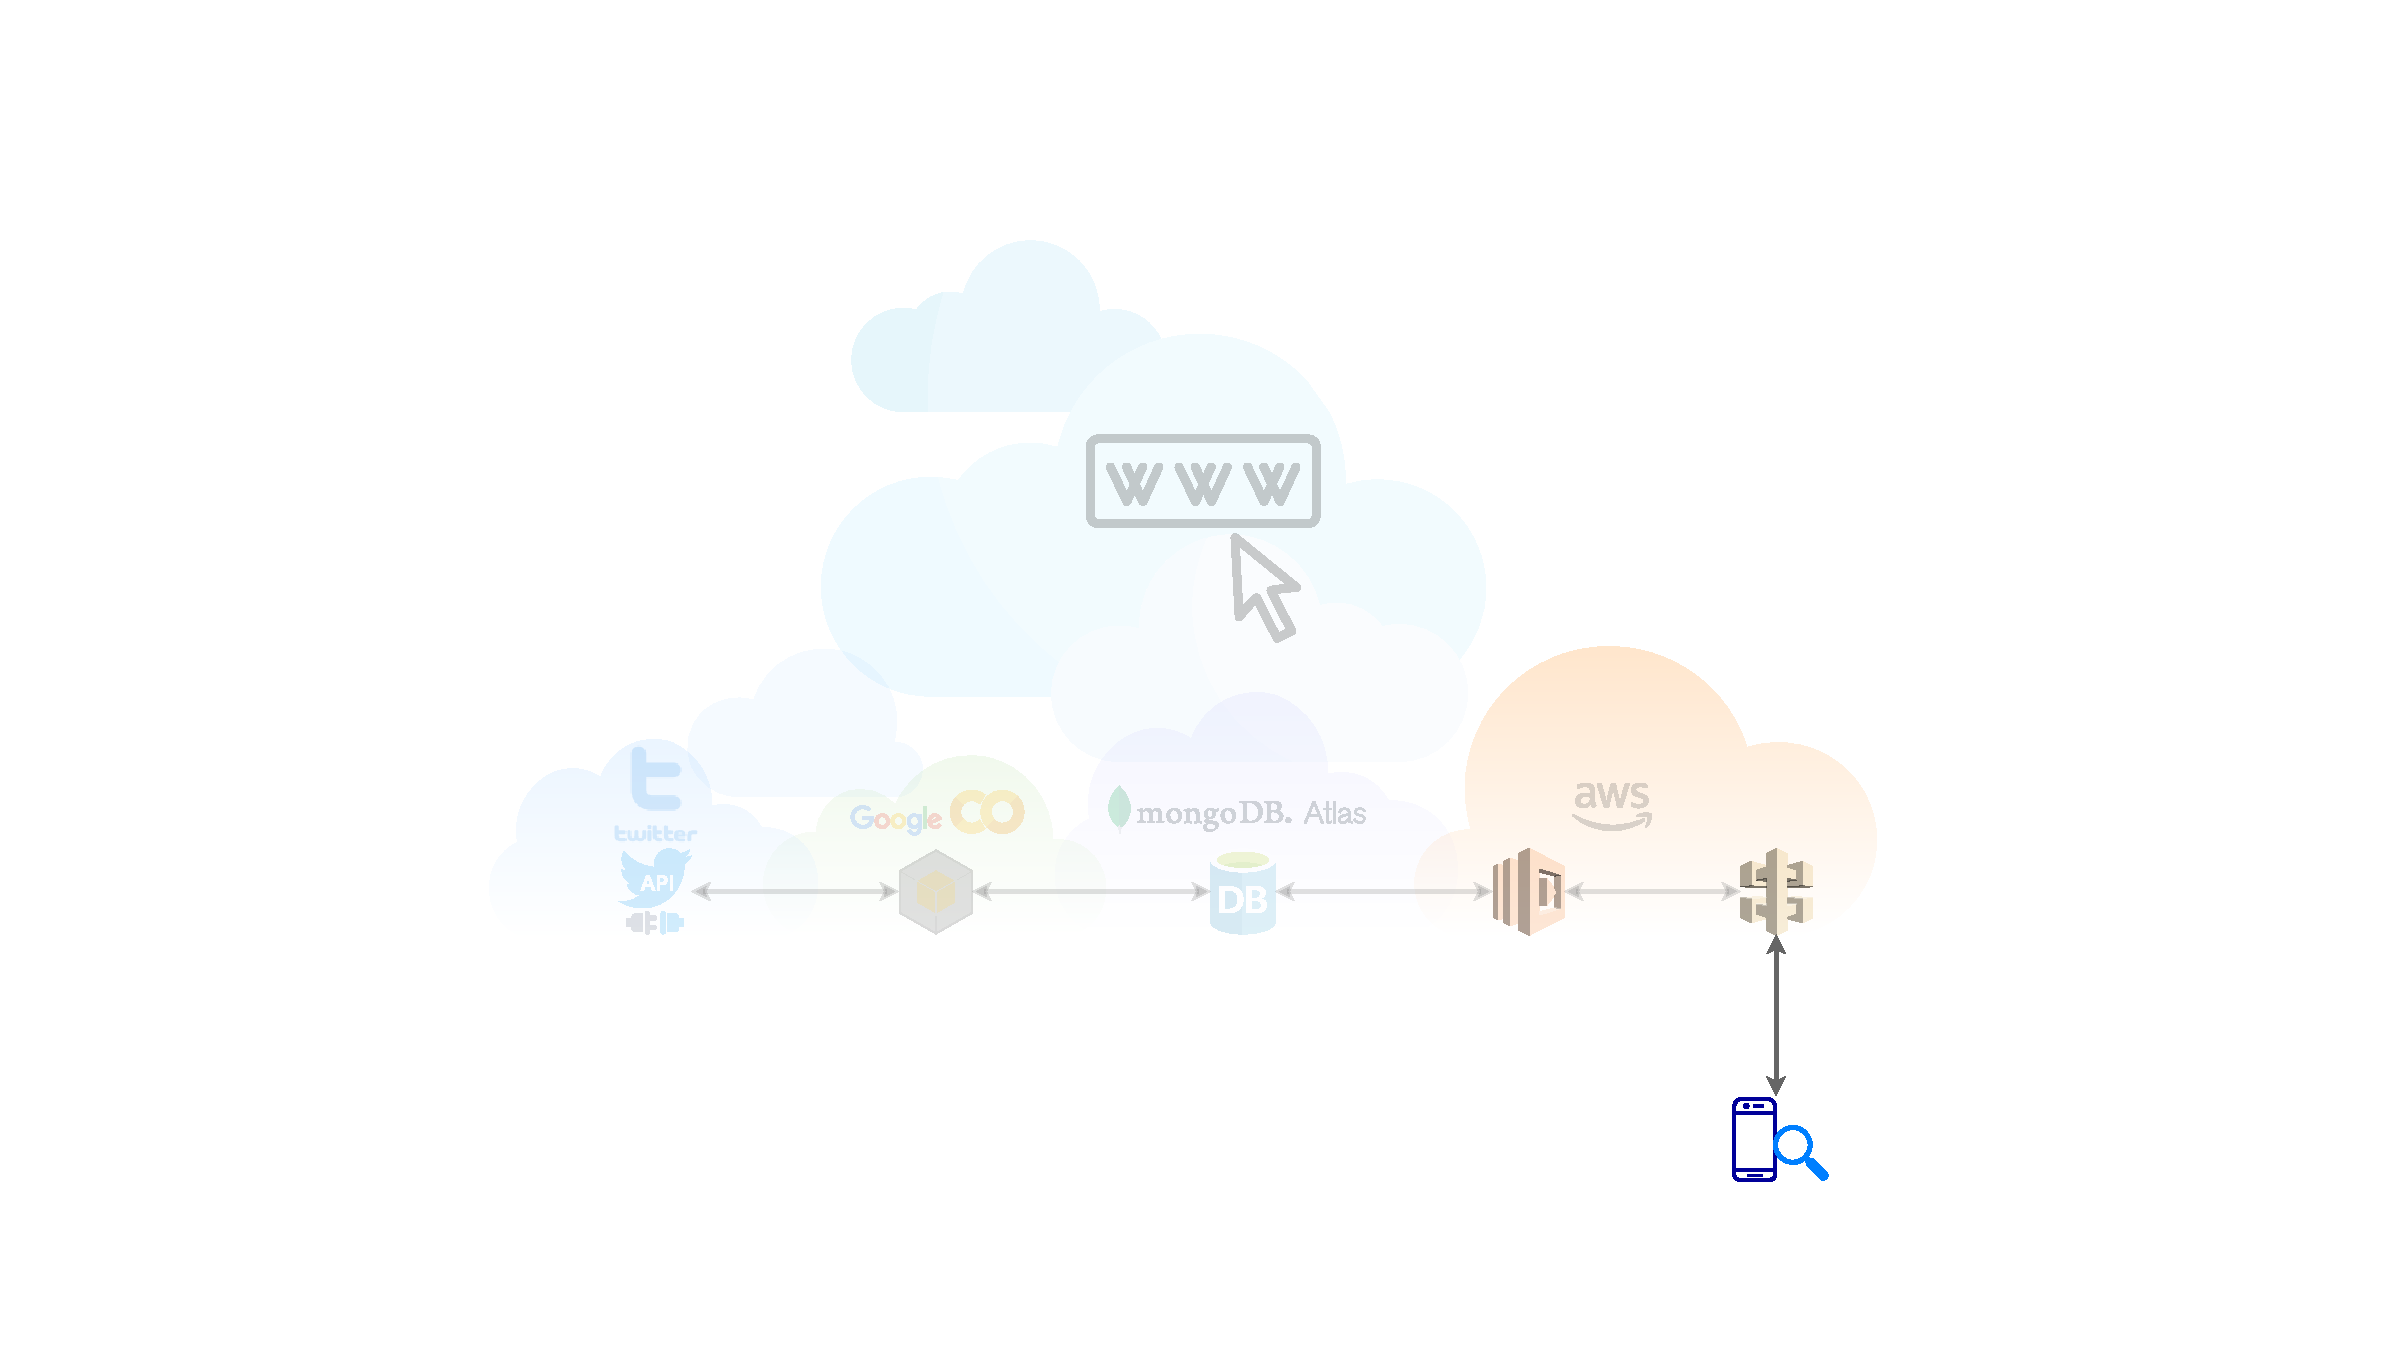
\includegraphics[width=1\paperwidth,height=1\paperheight,keepaspectratio]{Architectura_progetto_Mobile.pdf}
        }
    \end{figure}
\end{frame}

\subsection{Panoramica della WebApp}

%------------------------------------------------

\subsubsection{Tecnologie VueJS e Nuxt per sito web e progressive mobile app}

%------------------------------------------------

\subsubsection{Views e schermate durante l'esecuzione}

\begin{frame}{Schermata iniziale della WebApp}
    \begin{columns}[t]
        \column{.31\textwidth}
        Data di default settata a quella di oggi.\\~\\~\\
        
        Location di default settata a 'Worldwide', WOEID = 1.\\~\\~\\
        
        In automatico la WebApp mostra le trending topics del giorno nel mondo.
        
        \column{.32\textwidth}
        \vspace*{-18pt}
        \begin{figure}[H]
            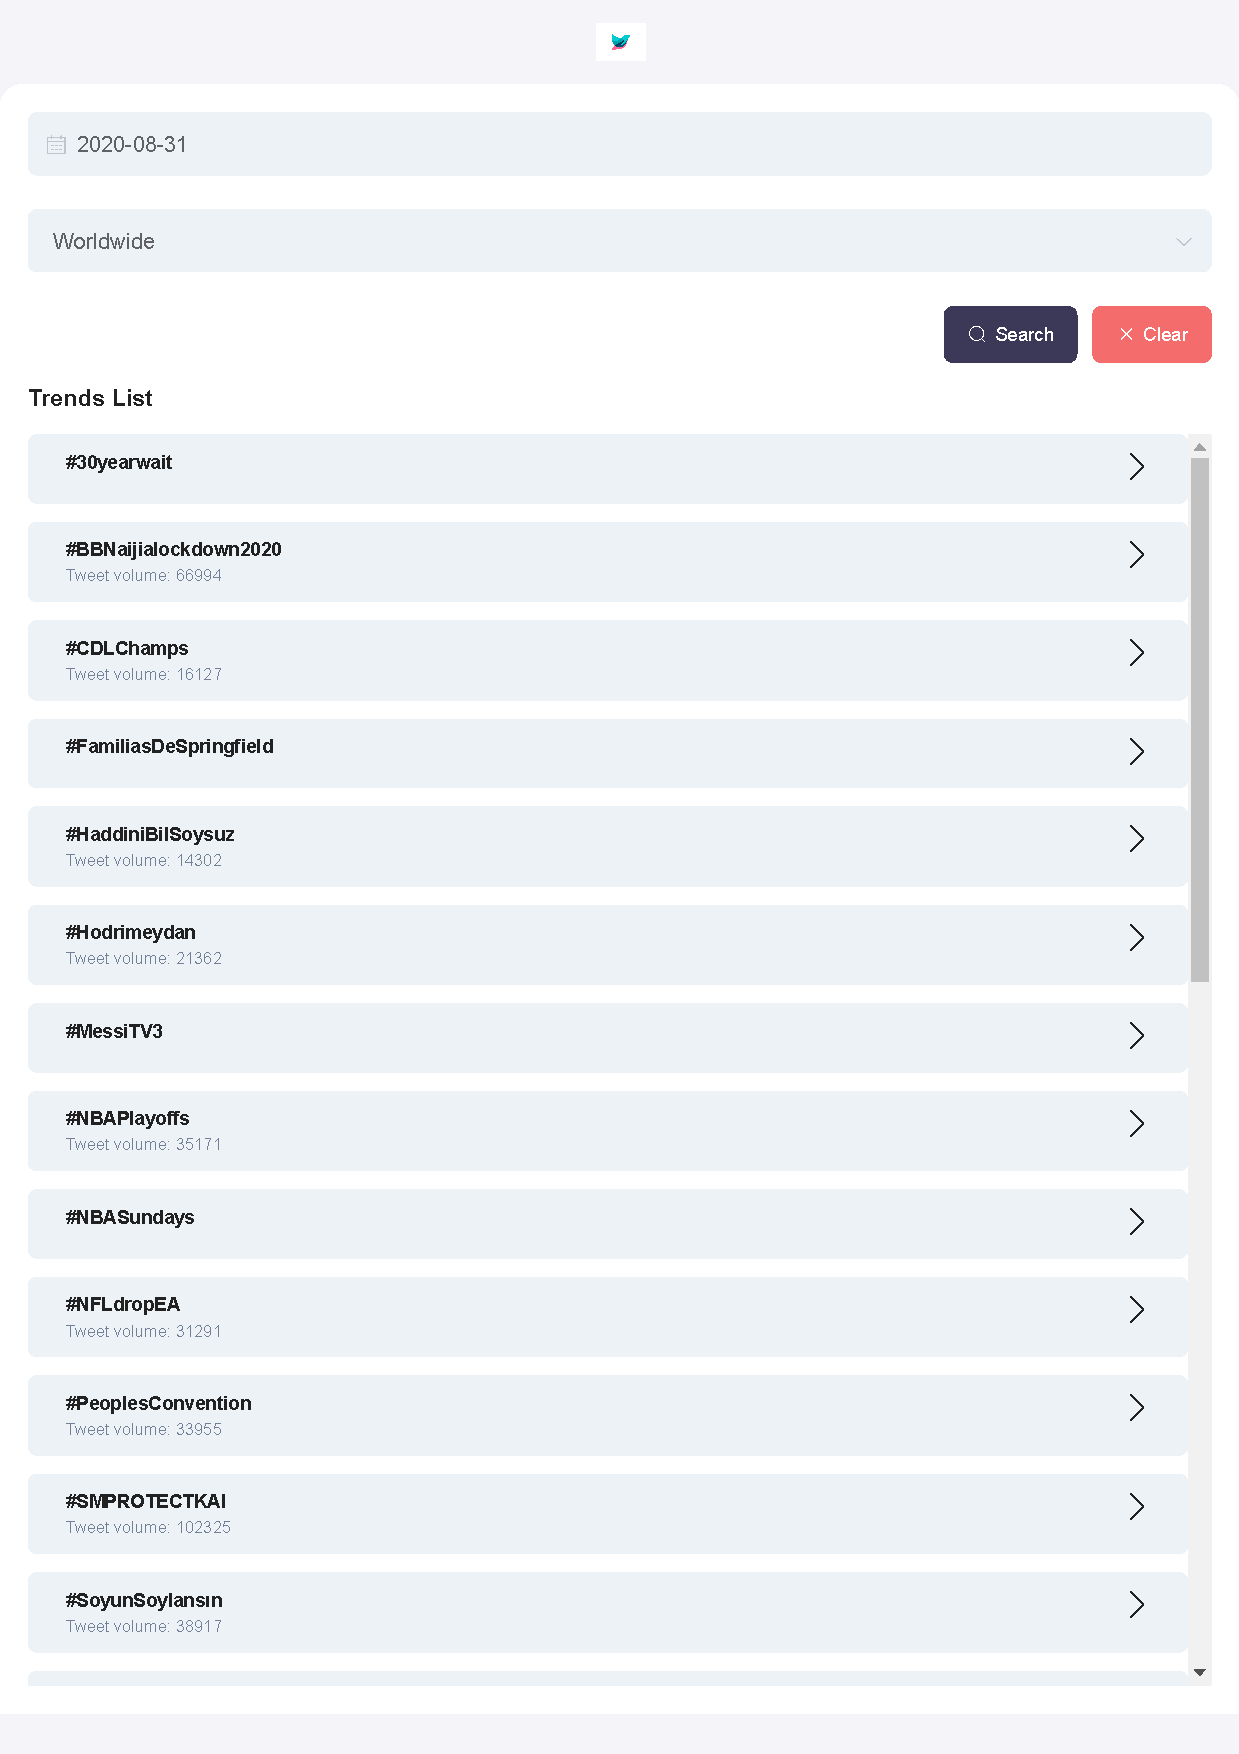
\includegraphics[width=0.75\paperwidth,height=0.75\paperheight,keepaspectratio]{FrontEnd_TrendrApp.pdf}
        \end{figure}
        \column{.32\textwidth}
        \vspace*{-18pt}
        \begin{figure}[H]
            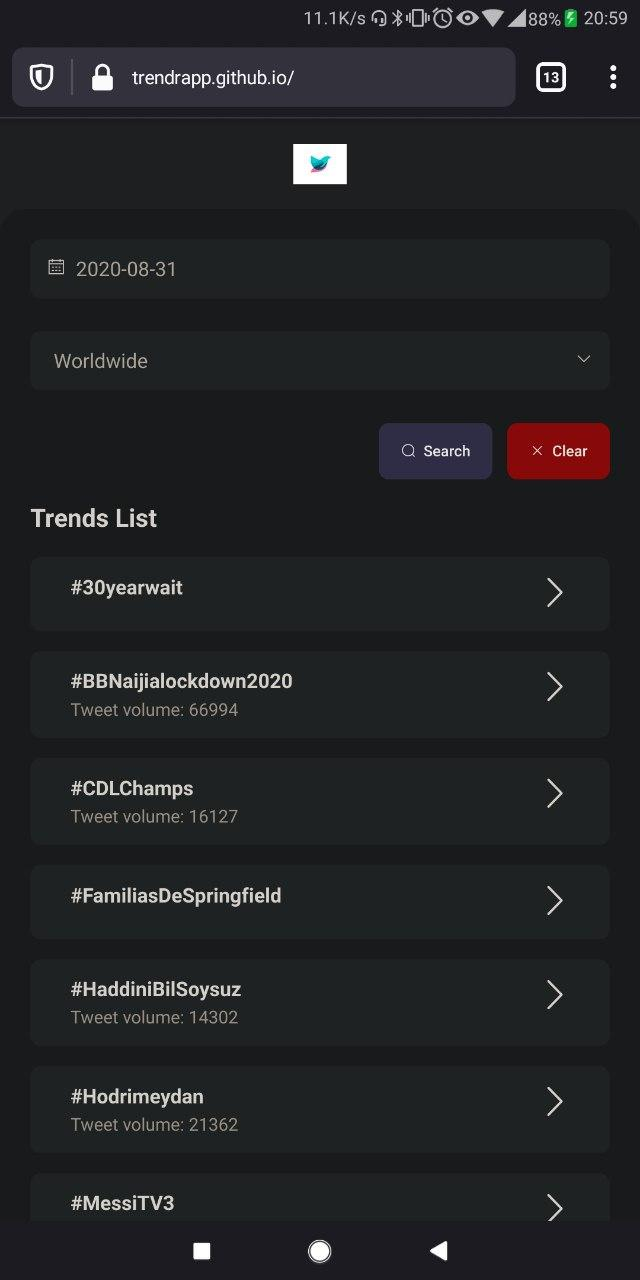
\includegraphics[width=0.75\paperwidth,height=0.75\paperheight,keepaspectratio]{Mobile_Firefox_Schermata_di_default.jpg}
        \end{figure}
    \end{columns}
\end{frame}

%------------------------------------------------

\subsection{Features}

\subsubsection{Installazione su mobile da browser}

\begin{frame}{Installazione su mobile da browser}
    Installazione su Mozilla Firefox e Chrome in mobile
    \begin{columns}[t]
        \column{.32\textwidth}
        \vspace*{-8pt}
        \begin{figure}[H]
            \centering
            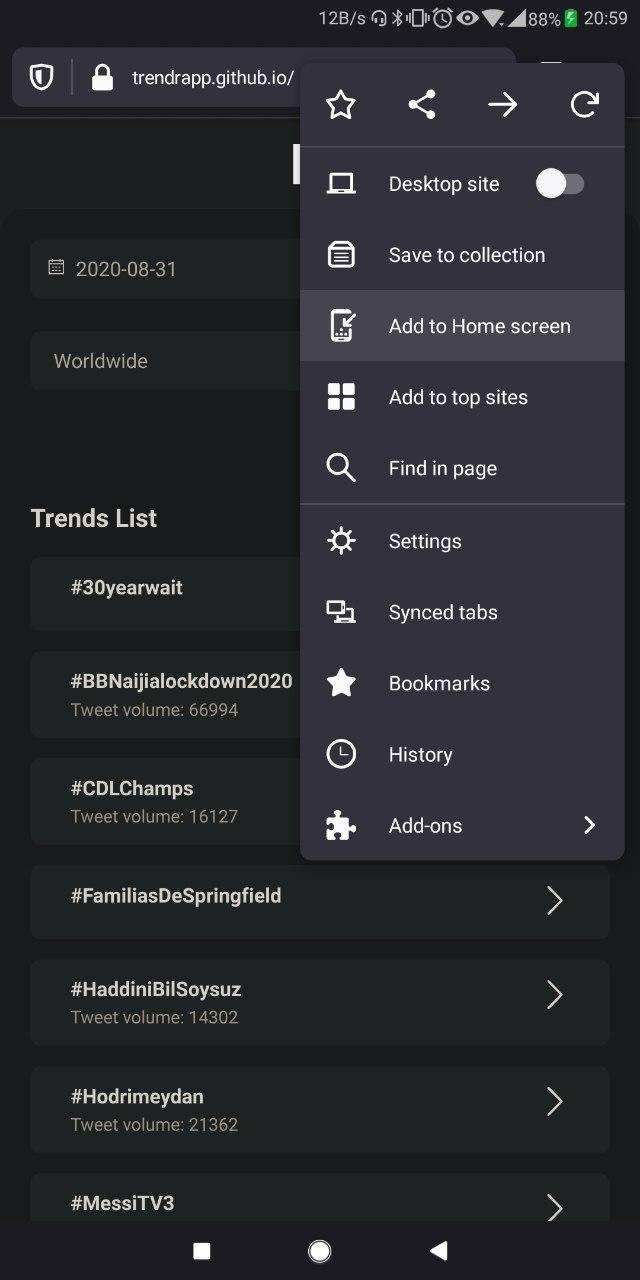
\includegraphics[width=0.32\paperwidth,height=0.7\paperheight,keepaspectratio]{Mobile_Firefox_Installazione_Menu_aggiungi.jpg}
        \end{figure}
        \column{.32\textwidth}
        \vspace*{-8pt}
        \begin{figure}[H]
            \centering
            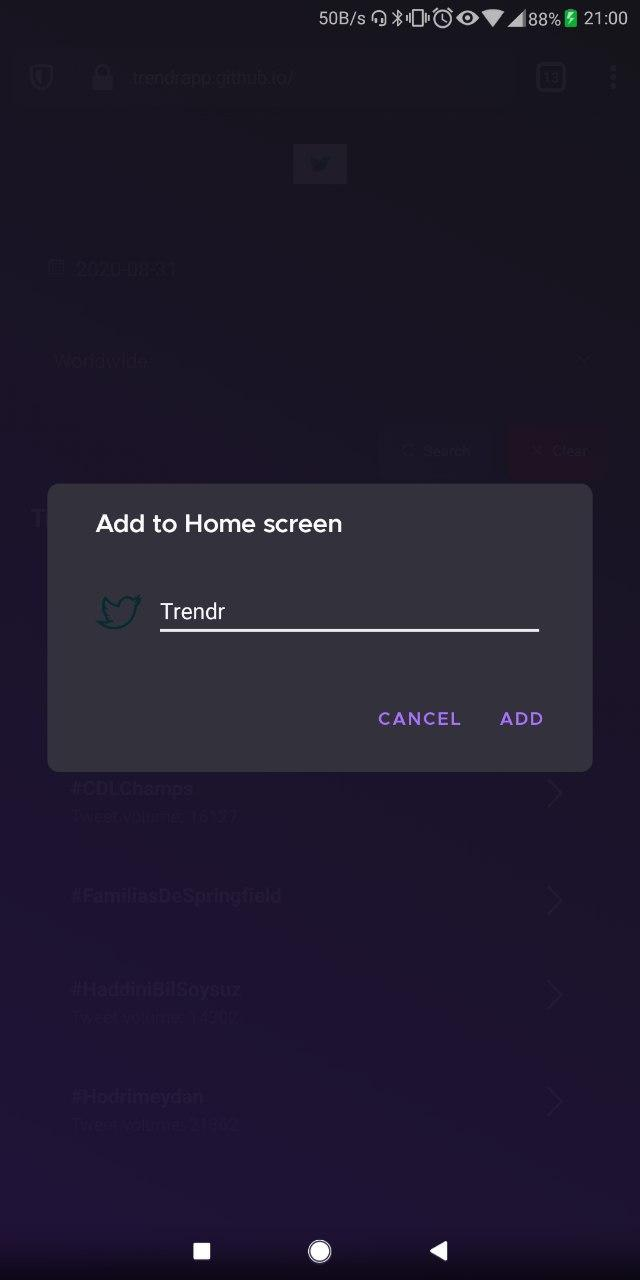
\includegraphics[width=0.32\paperwidth,height=0.7\paperheight,keepaspectratio]{Mobile_Firefox_Installazione_Conferma.jpg}
        \end{figure}
        \column{.32\textwidth}
        \vspace*{-8pt}
        \begin{figure}[H]
            \centering
            
\includegraphics[width=0.32\paperwidth,height=0.7\paperheight,keepaspectratio]{Immagini/Mobile_Icona_App_Installata.jpg}
        \end{figure}
    \end{columns}
\end{frame}

%------------------------------------------------

\subsubsection{Date disponibili con trends del passato}

\begin{frame}{Date disponibili con trends del passato}
    Scelta data in Web broser su desktop, in mobile su Firefox e Chrome.
    \begin{columns}[t]
        \column{.32\textwidth}
        \vspace*{-12pt}
        \begin{figure}[H]
            \centering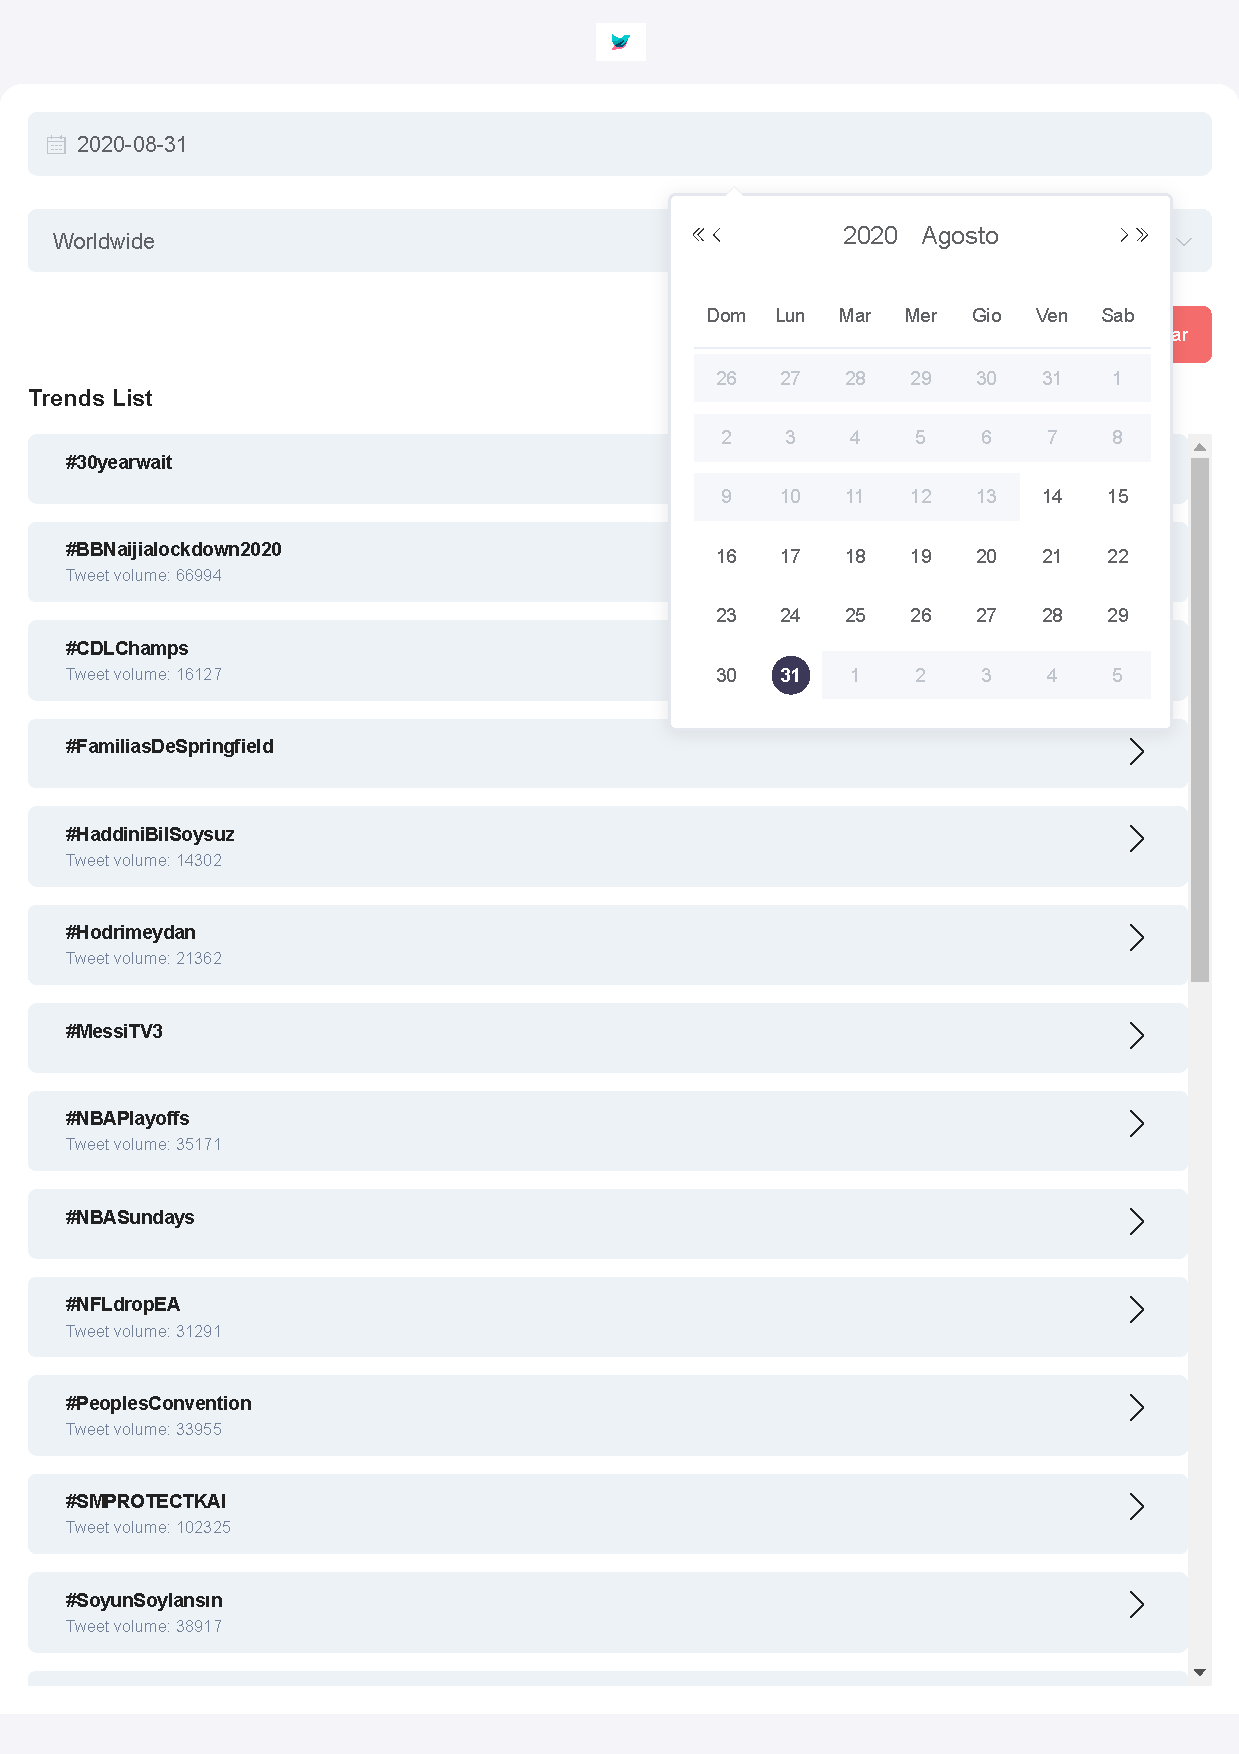
\includegraphics[width=0.32\paperwidth,height=0.65\paperheight,keepaspectratio]{FrontEnd_TrendrApp_Scelta_Data.pdf}
        \end{figure}
        \column{.32\textwidth}
        \vspace*{-12pt}
        \begin{figure}[H]
            \centering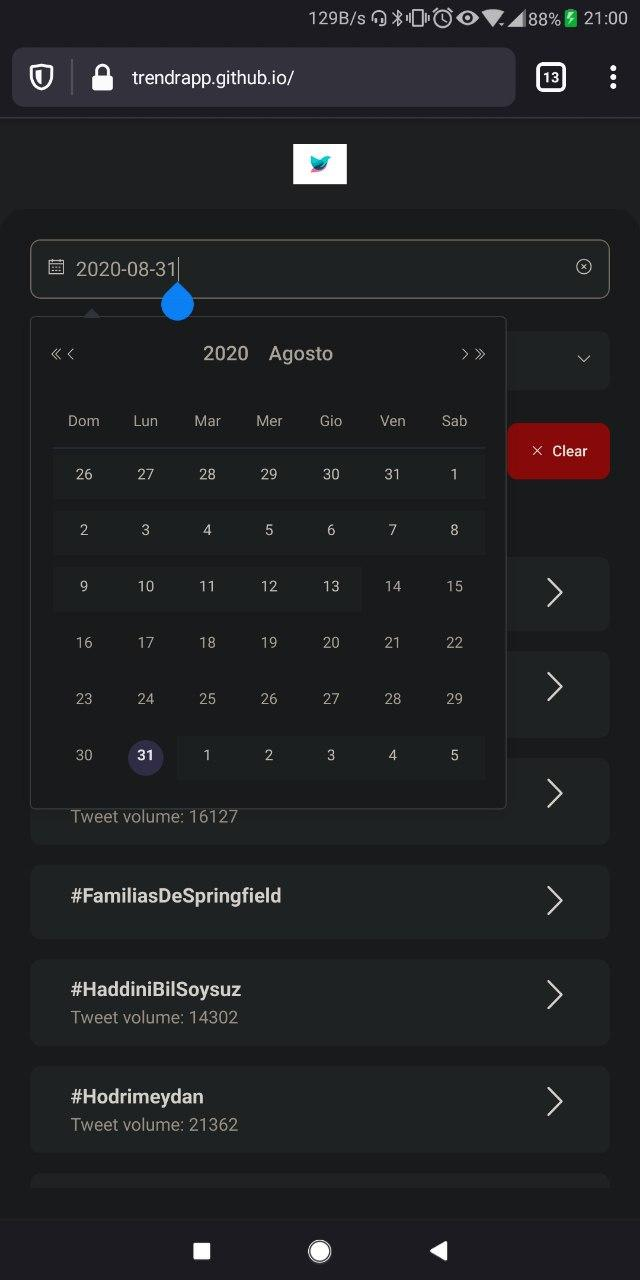
\includegraphics[width=0.32\paperwidth,height=0.65\paperheight,keepaspectratio]{Mobile_Firefox_Ricerca_Scelta_data.jpg}
        \end{figure}
        \column{.32\textwidth}
        \vspace*{-12pt}
        \begin{figure}[H]
            \centering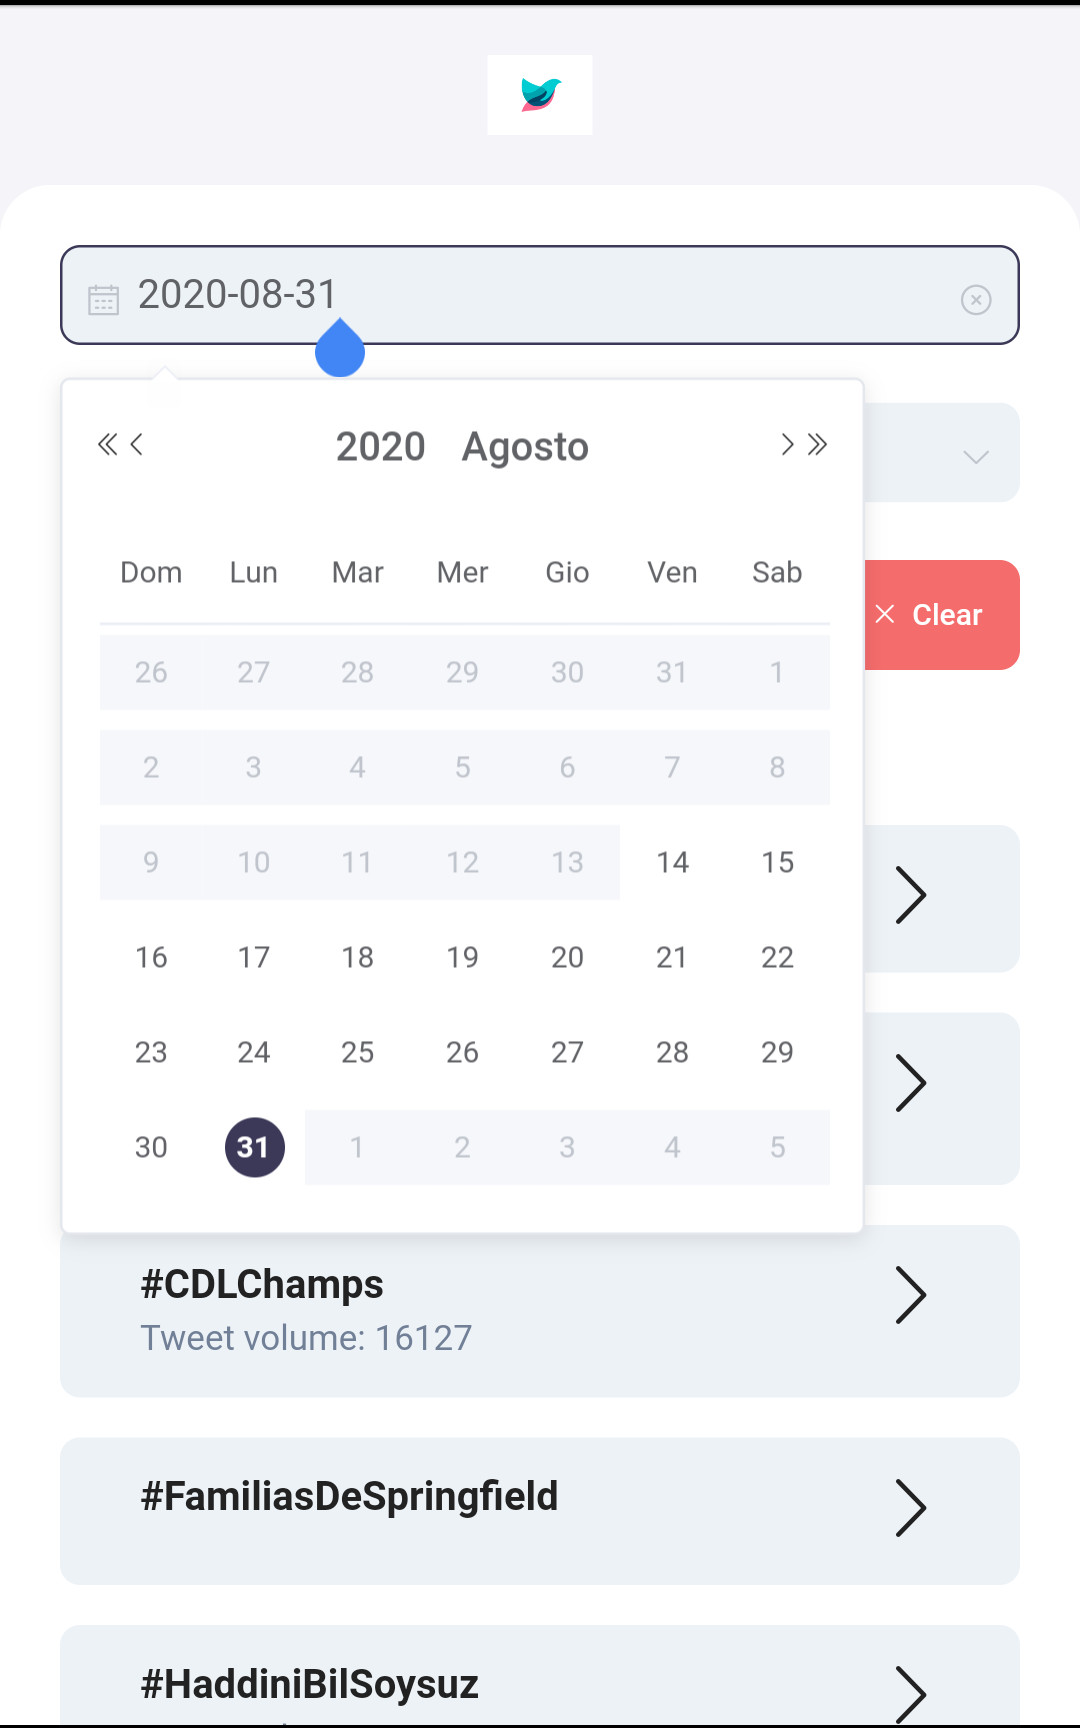
\includegraphics[width=0.32\paperwidth,height=0.65\paperheight,keepaspectratio]{Mobile_Chrome_Ricerca_Scelta_data.jpg}
        \end{figure}
    \end{columns}
\end{frame}

%------------------------------------------------

\begin{frame}{Data in formato ISO, detto anche militare (YYYY-MM-DD)}
    \begin{figure}[H]
        \centering
        \noindent\makebox[\textheight]{
            
\includegraphics[width=0.8\paperwidth,height=0.75\paperheight,keepaspectratio]{Meme_Perfect_Date_YYYY-MM-DD.jpg}
        }
    \end{figure}
\end{frame}

%------------------------------------------------

\subsubsection{Locations con trends, paesi e città}

\begin{frame}{Locations con trends, paesi}
    \begin{columns}[t]
        \column{.31\textwidth}
        
        \column{.64\textwidth}
        \vspace*{-24pt}
        \begin{figure}[H]
            \centering
            \noindent\makebox[\textheight]{
                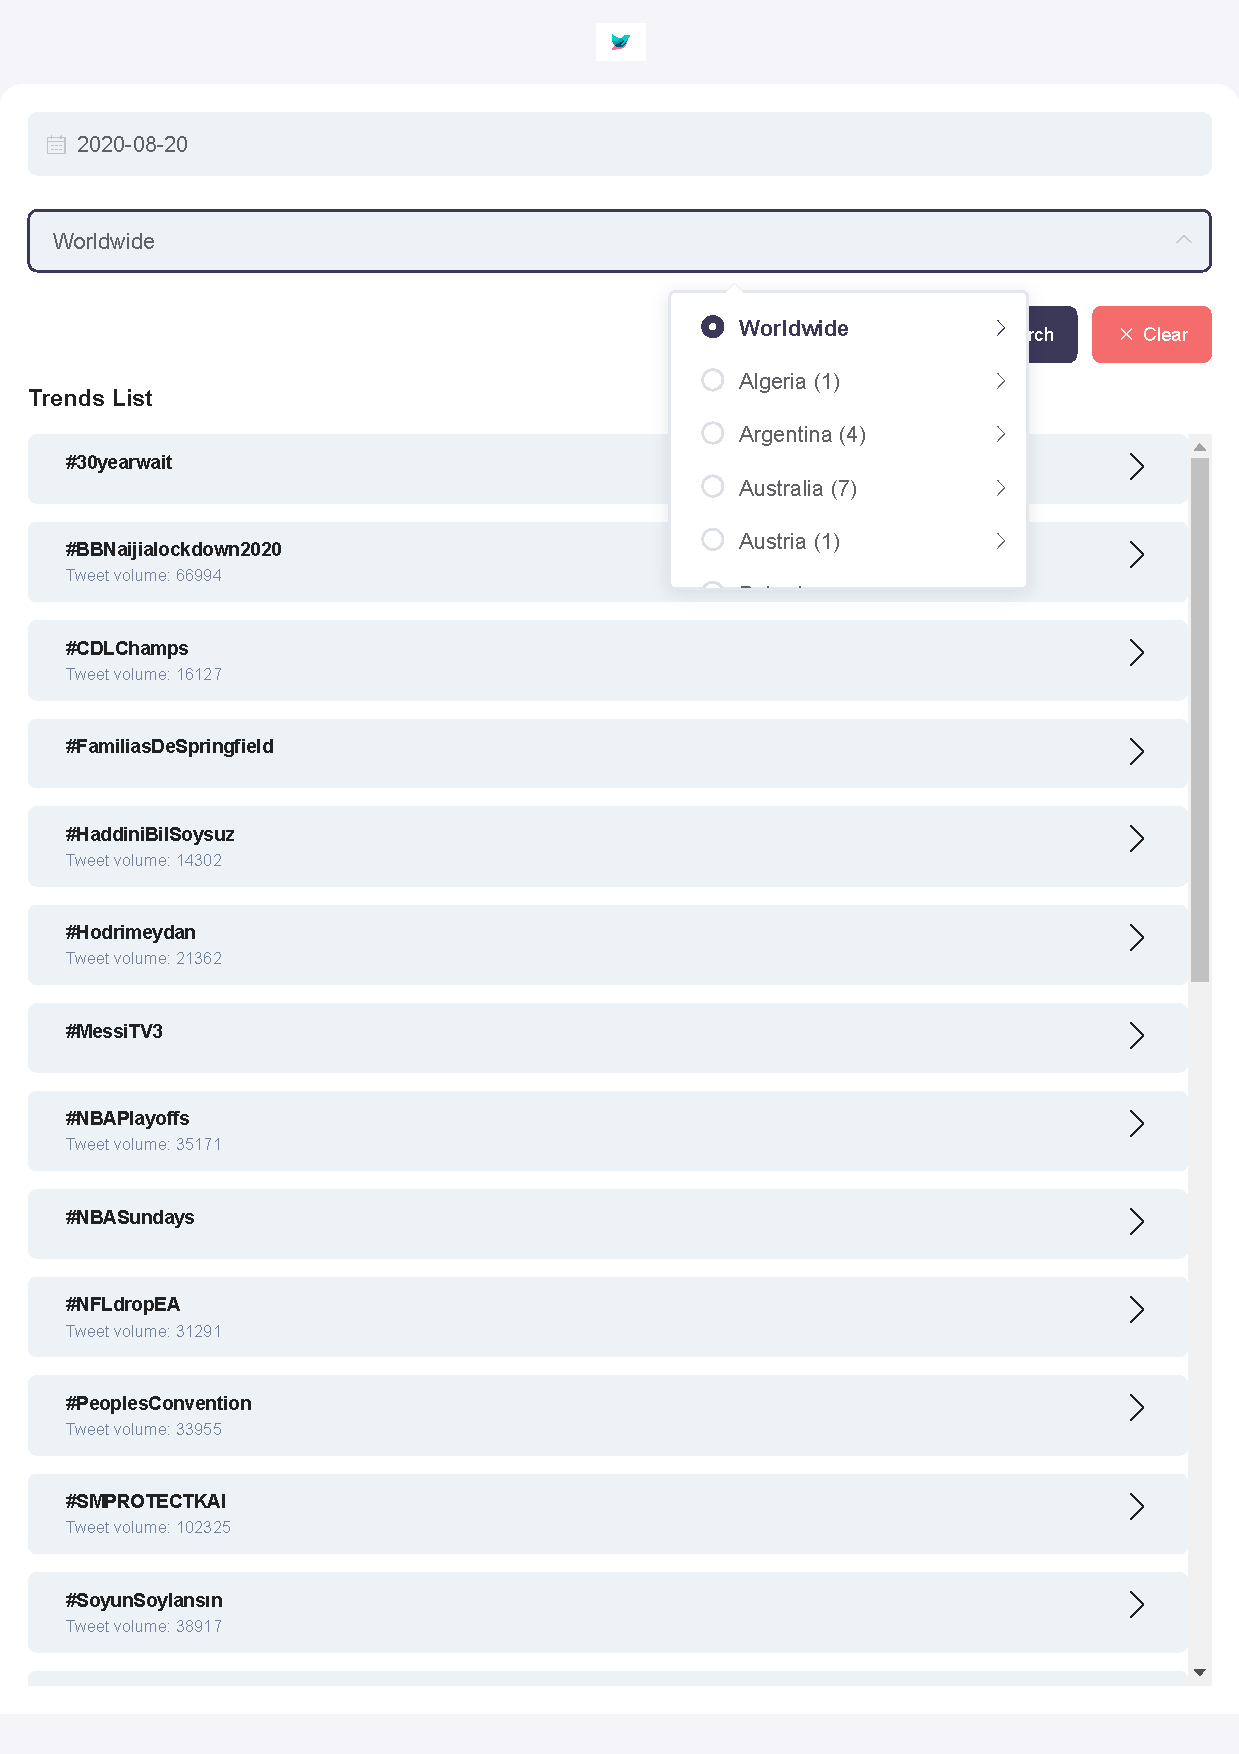
\includegraphics[width=0.75\paperwidth,height=0.75\paperheight,keepaspectratio]{FrontEnd_TrendrApp_Scelta_Location.pdf}
            }
        \end{figure}
    \end{columns}
\end{frame}

%------------------------------------------------

\begin{frame}{Locations con trends, paese - città}
    Non selezionato, poi Italia, Milano su Firefox per mobile e UK, Londra su Chrome per mobile
    \begin{columns}[t]
        \column{.32\textwidth}
        \vspace*{-12pt}
        \begin{figure}[H]
            \centering
            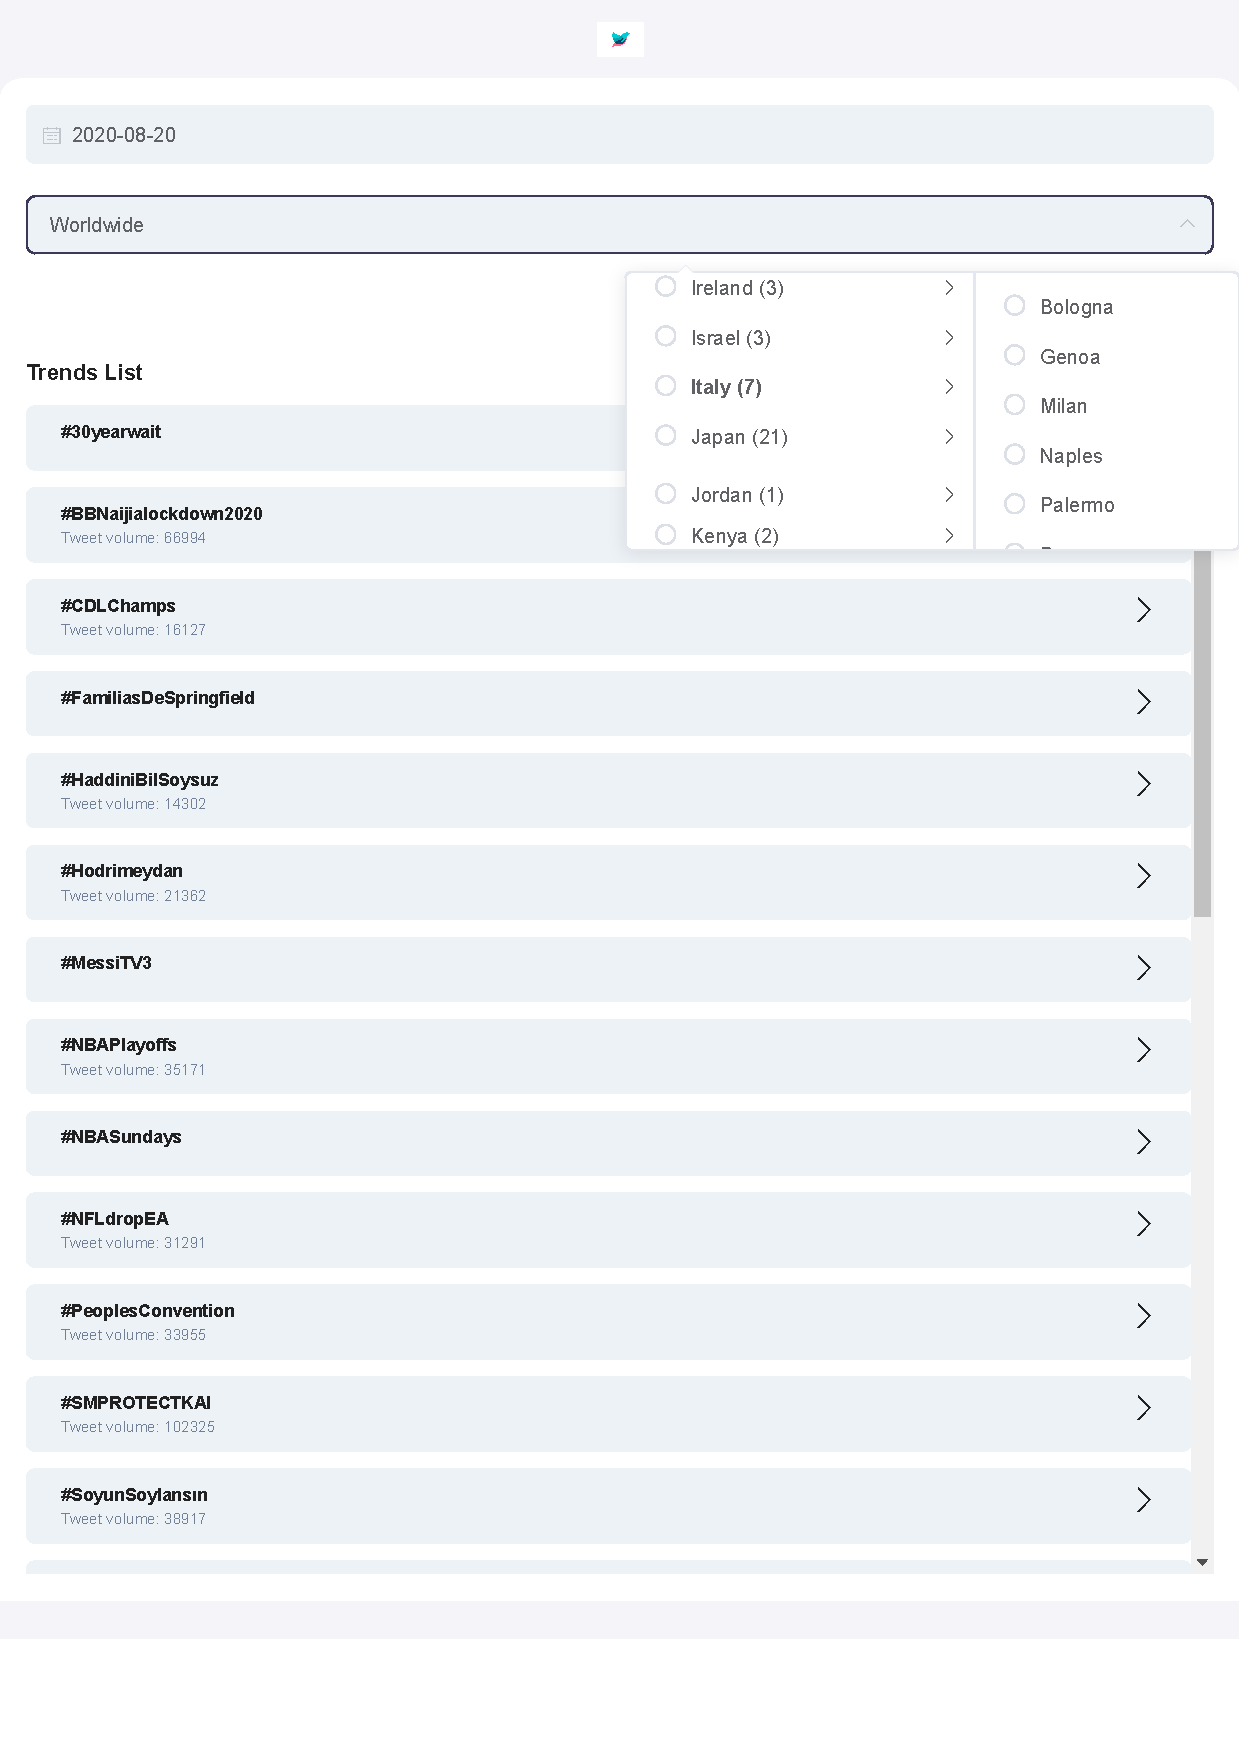
\includegraphics[width=0.32\paperwidth,height=0.7\paperheight,keepaspectratio]{FrontEnd_TrendrApp_Scelta_Location_Paese_City.pdf}
        \end{figure}
        \column{.32\textwidth}
        \vspace*{-12pt}
        \begin{figure}[H]
            \centering
            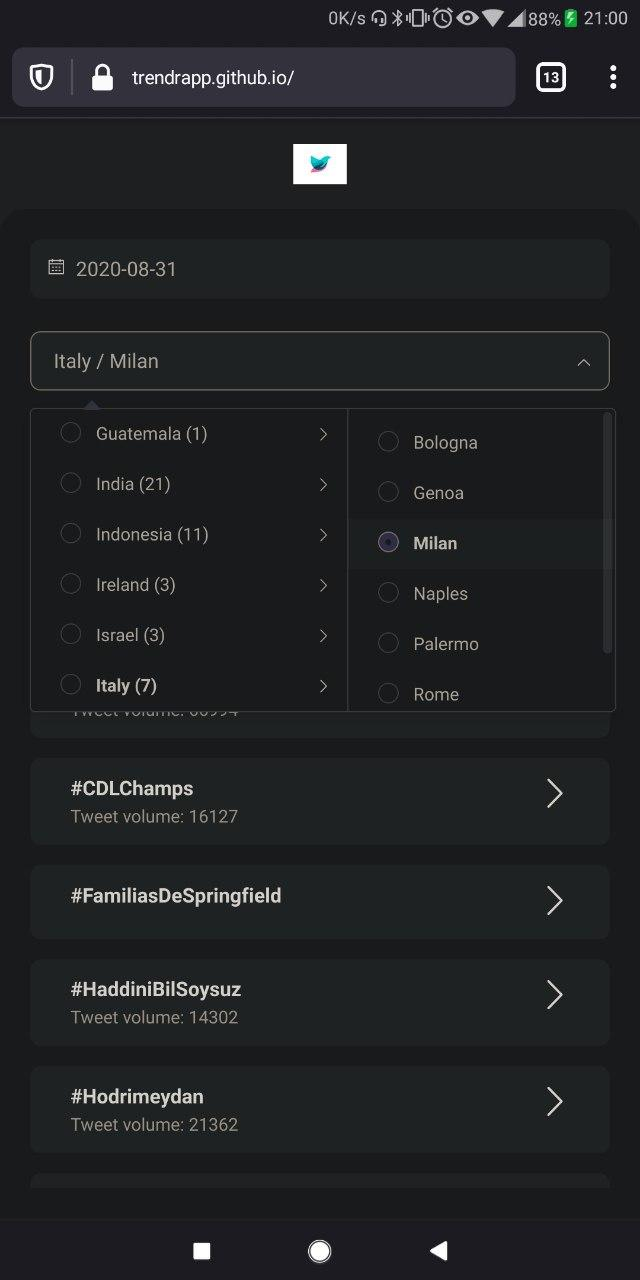
\includegraphics[width=0.32\paperwidth,height=0.7\paperheight,keepaspectratio]{Mobile_Firefox_Ricerca_Scelta_location_Italia_Milano.jpg}
        \end{figure}
        \column{.32\textwidth}
        \vspace*{-12pt}
        \begin{figure}[H]
            \centering
            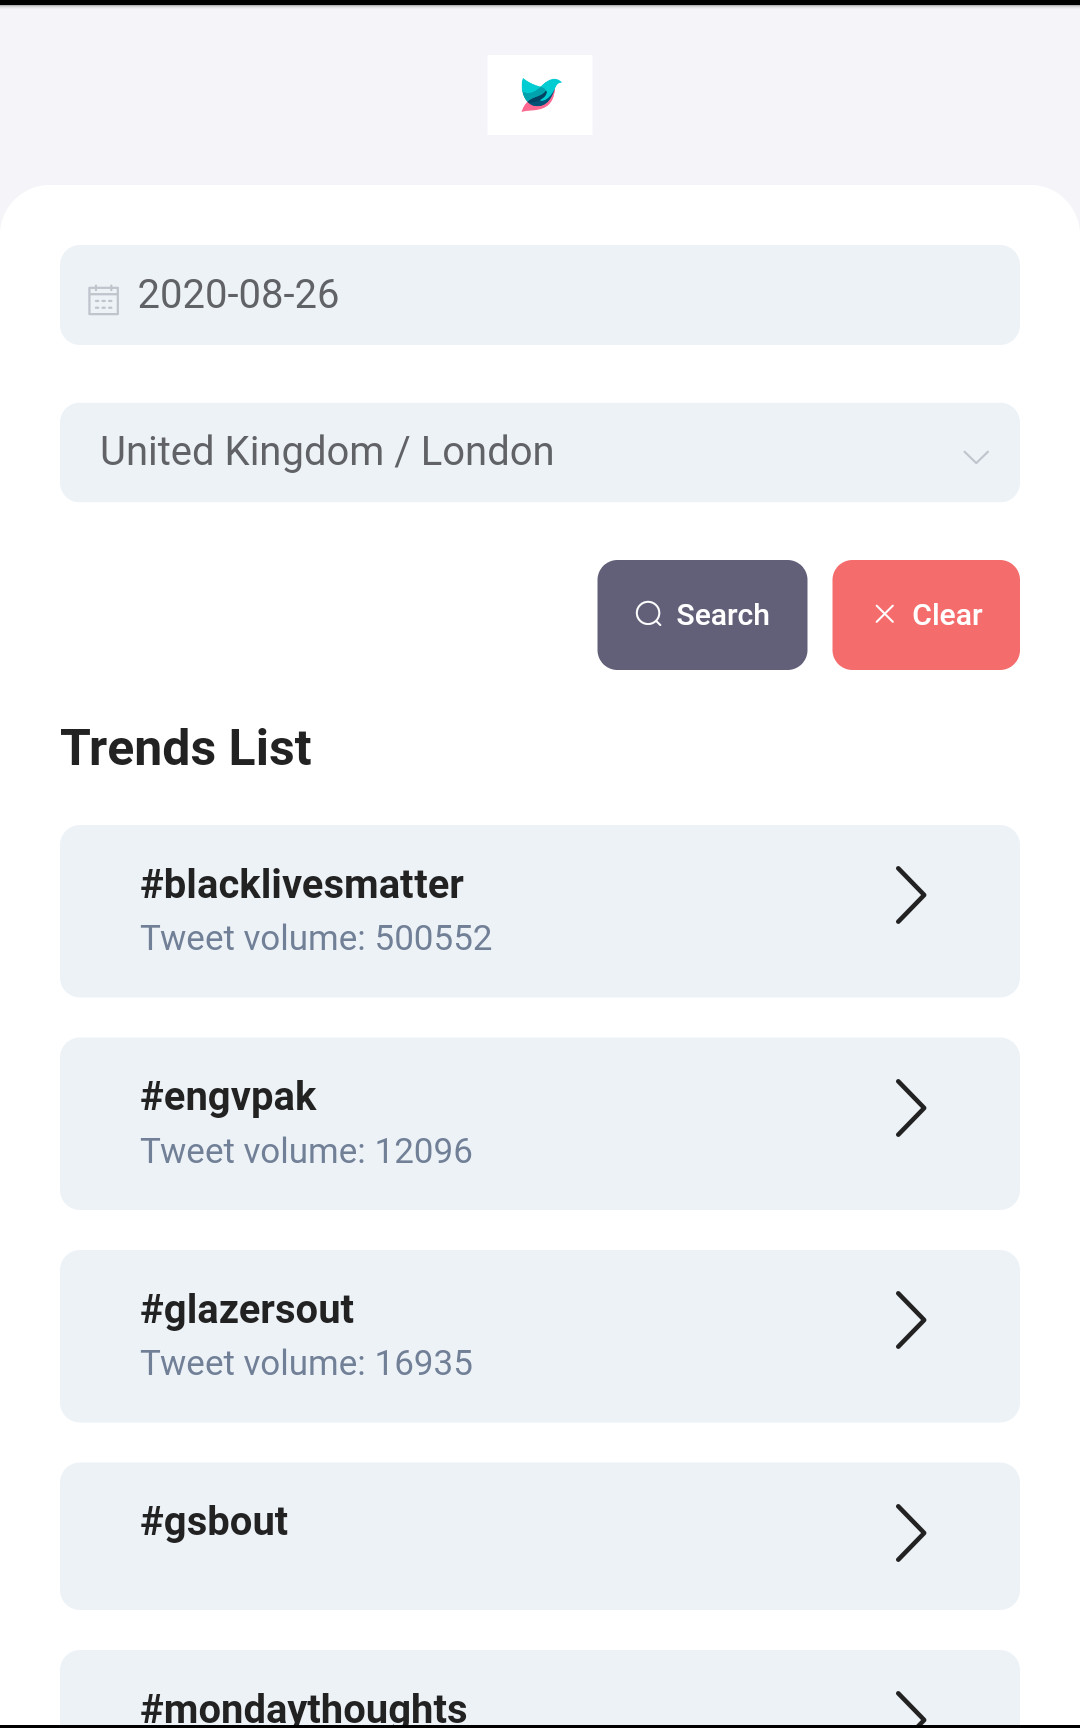
\includegraphics[width=0.32\paperwidth,height=0.7\paperheight,keepaspectratio]{Mobile_Chrome_Ricerca_trends_a_Londra_26_agosto.jpg}
        \end{figure}
    \end{columns}
\end{frame}

%------------------------------------------------

\subsubsection{Ricerca trends del passato}

\begin{frame}{Risultati di trends del passato}
    \begin{columns}[t]
        \column{.32\textwidth}
        \vspace*{-12pt}
        \begin{figure}[H]
            \centering
            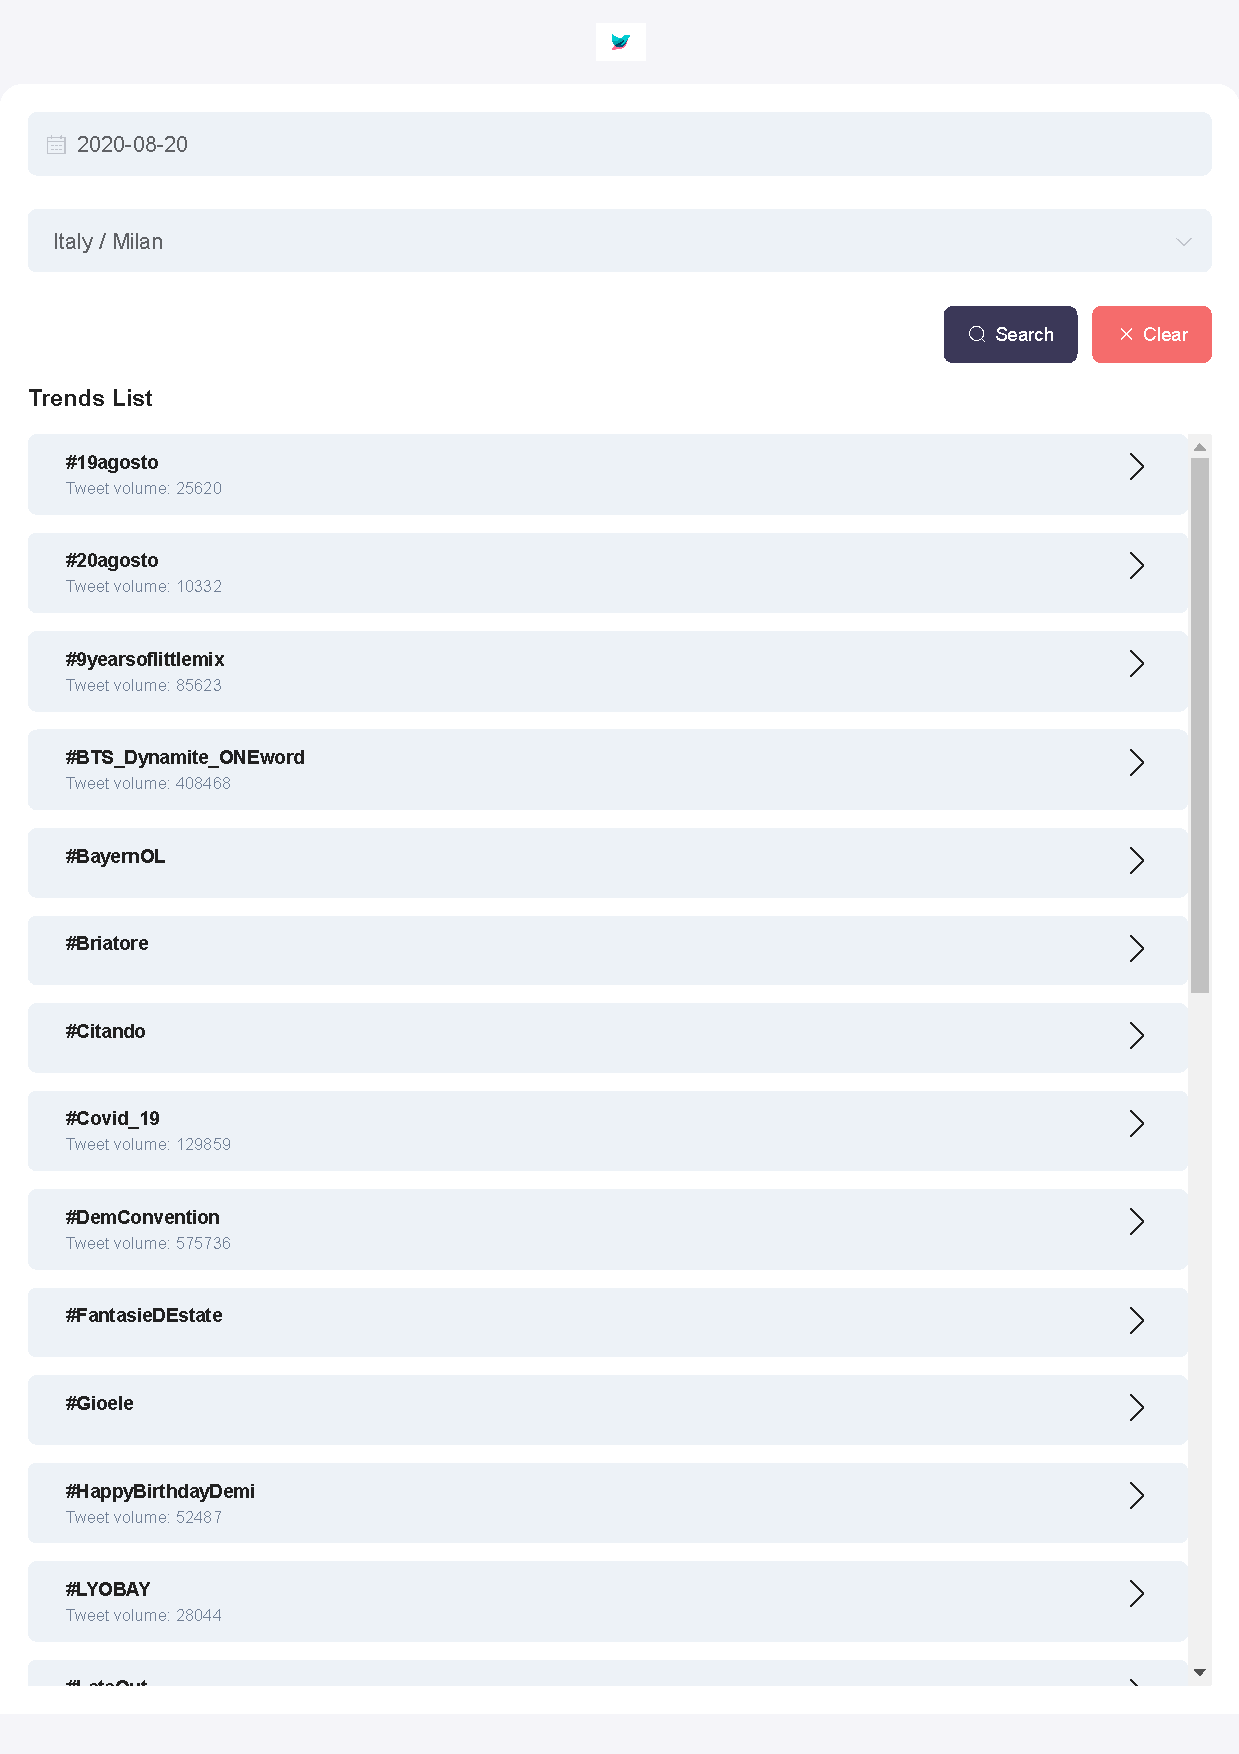
\includegraphics[width=0.32\paperwidth,height=0.7\paperheight,keepaspectratio]{Immagini/FrontEnd_TrendrApp_Scelta_Location_Paese_City_Risultati.pdf}
        \end{figure}
        \column{.32\textwidth}
        \vspace*{-12pt}
        \begin{figure}[H]
            \centering
            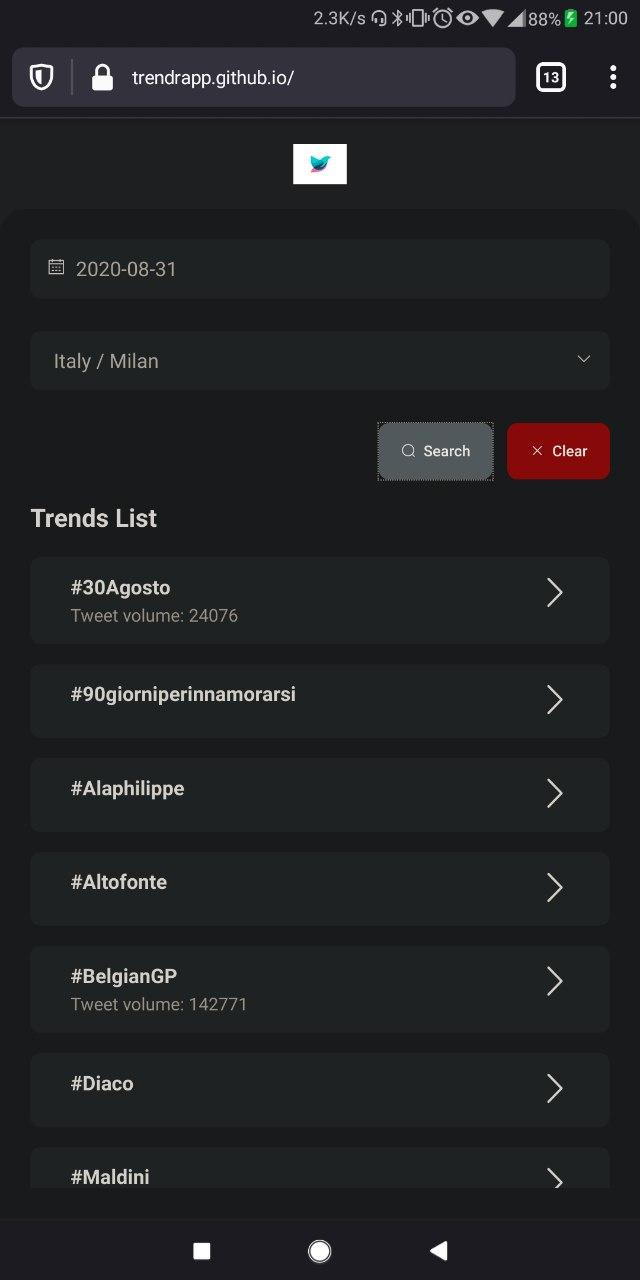
\includegraphics[width=0.32\paperwidth,height=0.7\paperheight,keepaspectratio]{Mobile_Firefox_Ricerca_trends_a_Milano_31_agosto.jpg}
        \end{figure}
        \column{.32\textwidth}
        \vspace*{-12pt}
        \begin{figure}[H]
            \centering
            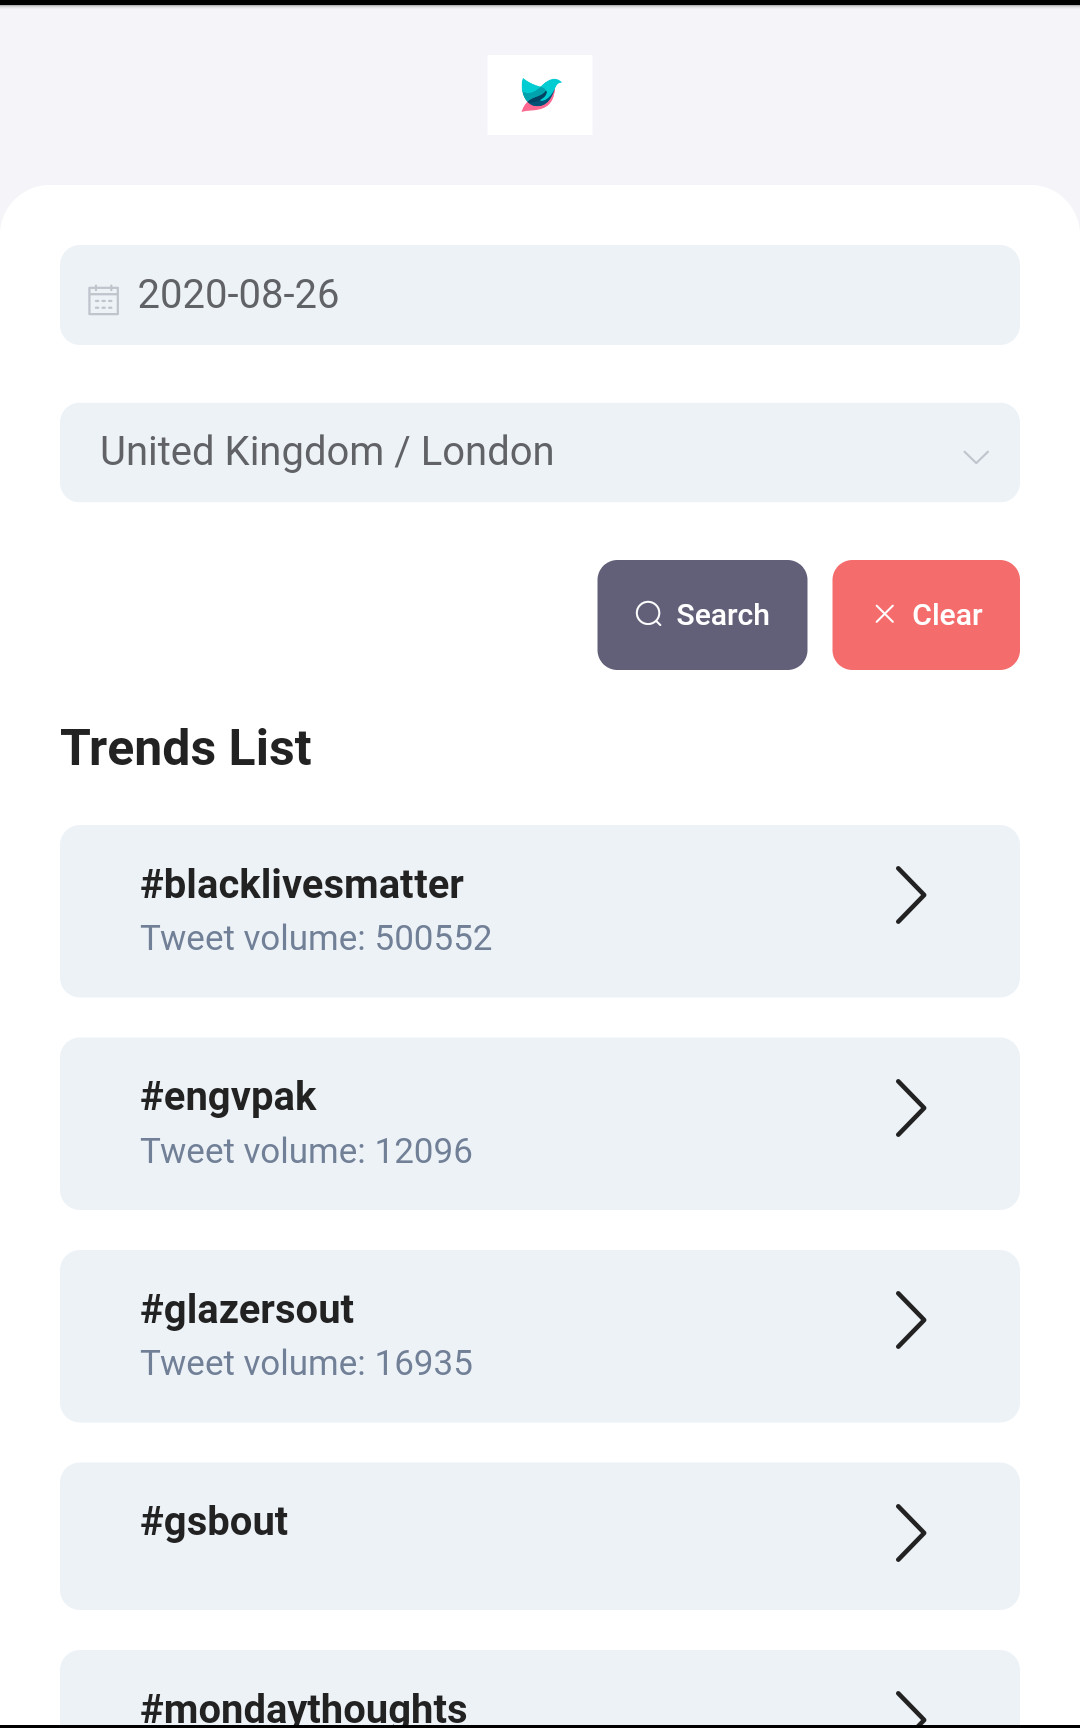
\includegraphics[width=0.32\paperwidth,height=0.7\paperheight,keepaspectratio]{Mobile_Chrome_Ricerca_trends_a_Londra_26_agosto.jpg}
        \end{figure}
    \end{columns}
\end{frame}

%------------------------------------------------

\subsubsection{Lazy loading, infinite scroll}

\begin{frame}{Lazy loading, infinite scroll}
    \begin{columns}[t]
        \column{.475\textwidth}
        \vspace*{-12pt}
        \begin{figure}[H]
            \centering
            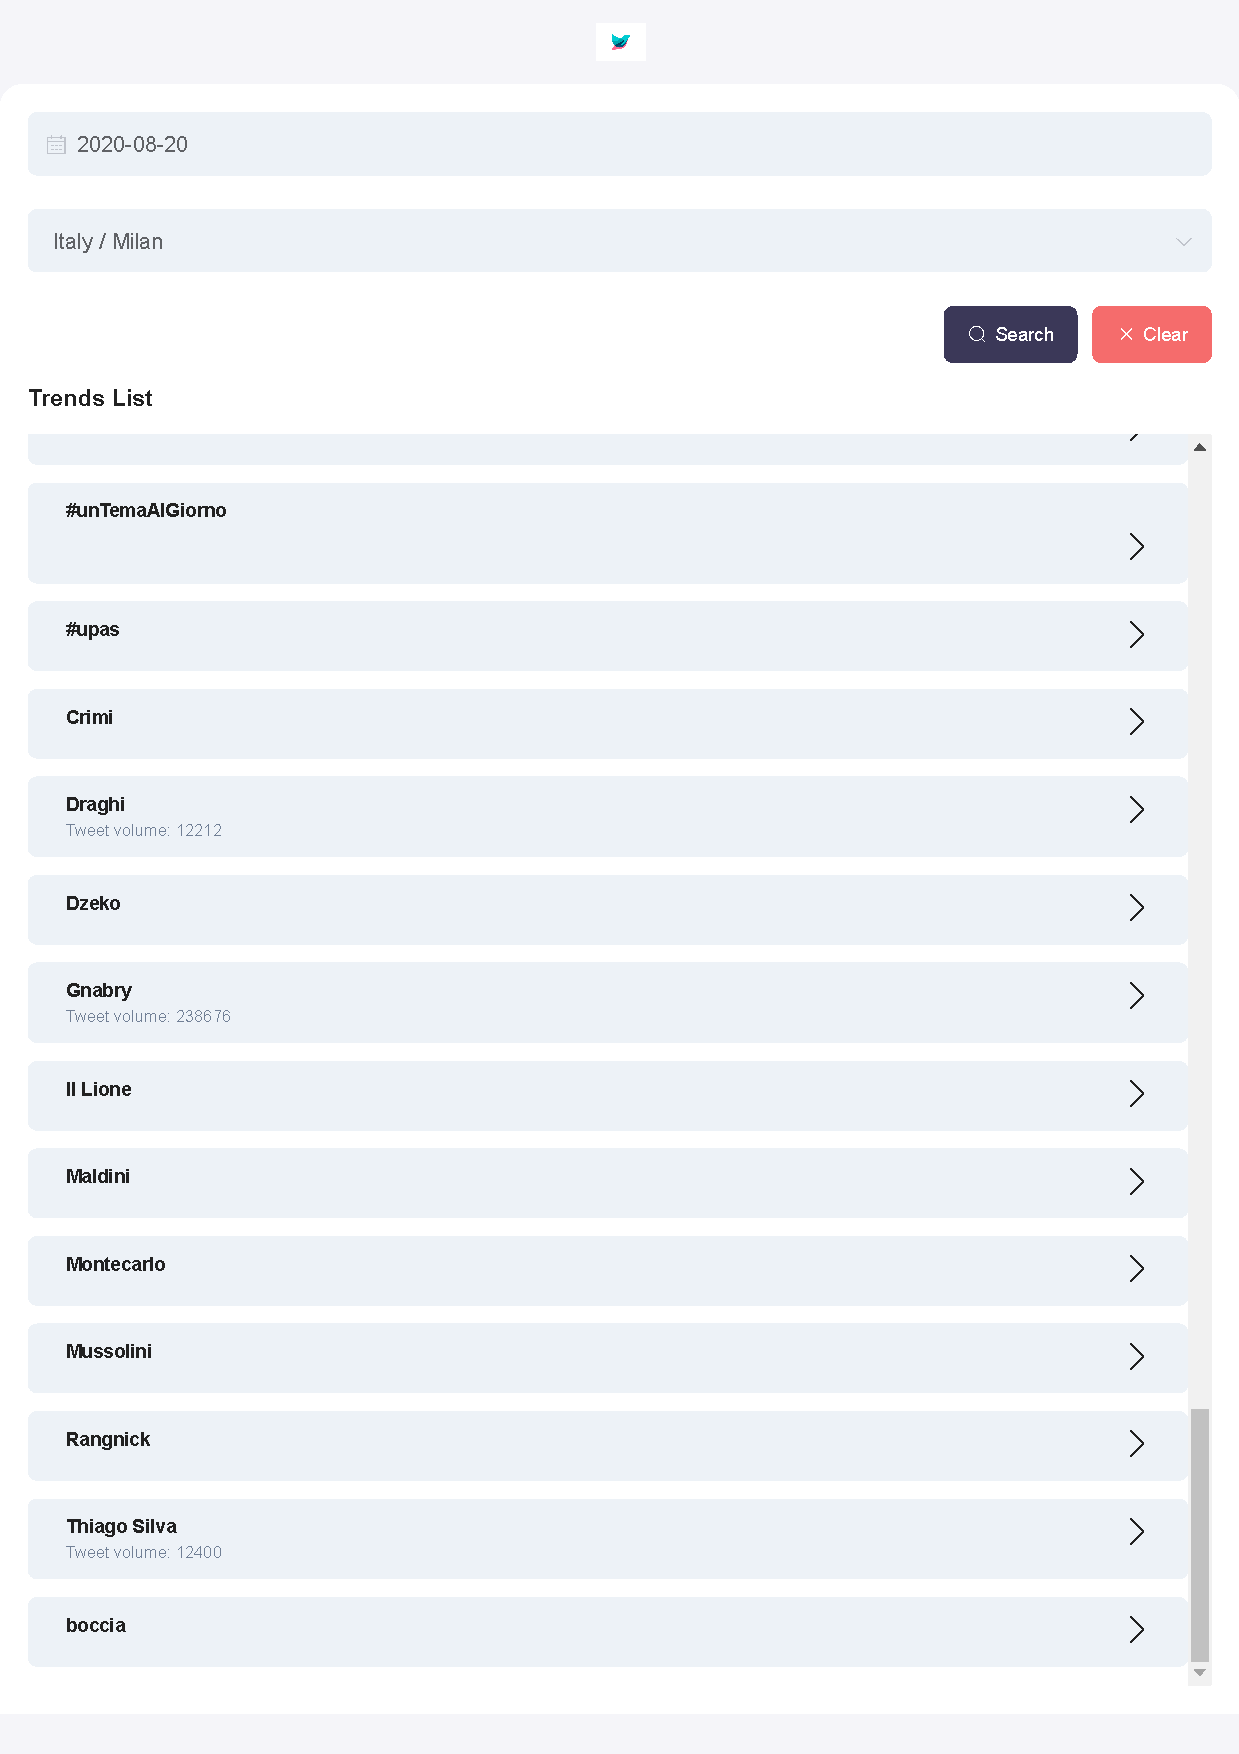
\includegraphics[width=0.475\paperwidth,height=0.7\paperheight,keepaspectratio]{Immagini/FrontEnd_TrendrApp_Scelta_Location_Paese_City_Risultati_Scroll.pdf}
        \end{figure}
        \column{.475\textwidth}
        \vspace*{-12pt}
        \begin{figure}[H]
            \centering
            \includegraphics[width=0.475\paperwidth,height=0.7\paperheight,keepaspectratio]{Mobile_Chrome_Trends_list_Lazy_loading_Infinite_scroll.jpg}
        \end{figure}
    \end{columns}
\end{frame}

%------------------------------------------------

\begin{frame}{Apertura di un risultato dalla lista dei trends}
    \begin{columns}[t]
        \column{.31\textwidth}
        Il trend si apre in una nuova tab o nel browser di default se in mobile.
        
        \column{.64\textwidth}
        \vspace*{-24pt}
        \begin{figure}[H]
            \centering
            \noindent\makebox[\textheight]{
                \includegraphics[width=0.75\paperwidth,height=0.75\paperheight,keepaspectratio]{FrontEnd_TrendrApp_Apertura_30yearwait.pdf}
            }
        \end{figure}
    \end{columns}
\end{frame}

%------------------------------------------------

\section{Deployment \& Demo}

\begin{frame}{\secname}
    \tableofcontents[sections={\thesection}, subsubsectionstyle=show, sectionstyle=hide]
\end{frame}

%------------------------------------------------

\subsection{Deployment della WebApp}

\begin{frame}{Deployment della Progressive WebApp su GitHub Pages}
    \vspace*{-6pt}
    \begin{figure}[H]
        \centering
            \includegraphics[width=0.75\paperwidth,height=0.75\paperheight,keepaspectratio]{trendrapp.github.io.pdf}
    \end{figure}
\end{frame}

%------------------------------------------------

\subsection{Live Demo}

\begin{frame}{Live demonstration del funzionamento della WebApp}
    \hspace*{150pt}\emph{page intentionally left blank}
\end{frame}

%------------------------------------------------

\section{Crediti}

\begin{frame}{\secname}
    \tableofcontents[sections={\thesection}, subsubsectionstyle=show, sectionstyle=hide]
\end{frame}

%------------------------------------------------

\subsection{Ringraziamenti}

\begin{frame}{Ringrazio...}
    \begin{block}{Mauro Pelucchi, Prof.}
        per la sua prontezza e disponibilità nell'aiutare a capire meglio i concetti di Cloud Computing su Amazon Web Services e i suoi suggerimenti riguardo i trade-offs da accettare nella progettazione del programma.
    \end{block}
\end{frame}

%------------------------------------------------

\begin{frame}{Fine}
    \begin{figure}[H]
        \vspace*{-6ex}
        \centering
        \noindent
        \makebox[\textwidth]{
            \includegraphics[width=1\paperwidth,height=1\paperheight-3.65ex]{Fine_Thats_all_folks.jpg}
        }
    \end{figure}
\end{frame}


%\begin{frame}{Fine}
%    \vspace*{-28pt}
%    \begin{figure}[H]
%        \centering
%        \noindent
%        \makebox[\textwidth]{
%            \includegraphics[width=1\paperwidth,height=1\paperheight,keepaspectratio]{Fine_Thats_all_folks.jpg}
%        }
%    \end{figure}
%\end{frame}

%------------------------------------------------

\end{document} 